%&preformat-disser
\RequirePackage[l2tabu,orthodox]{nag} % Раскомментировав, можно в логе получать рекомендации относительно правильного использования пакетов и предупреждения об устаревших и нерекомендуемых пакетах
% Формат А4, 14pt (ГОСТ Р 7.0.11-2011, 5.3.6)
\documentclass[a4paper,14pt,oneside,openany]{memoir}

\input{common/setup}               % общие настройки шаблона
%%% Поля и разметка страницы %%%
\usepackage{lscape}		% Для включения альбомных страниц
\usepackage{geometry}	% Для последующего задания полей

%%% Кодировки и шрифты %%%
\usepackage{cmap}						% Улучшенный поиск русских слов в полученном pdf-файле
%\usepackage[T2A]{fontenc}				% Поддержка русских букв
\usepackage{fontenc}				% Поддержка русских букв
\usepackage[utf8]{inputenc}				% Кодировка utf8
\usepackage[english, russian]{babel}	% Языки: русский, английский
%\usepackage{pscyr}						% Красивые русские шрифты

%%% Математические пакеты %%%
\usepackage{amsthm,amsfonts,amsmath,amssymb,amscd} % Математические дополнения от AMS

%%% Оформление абзацев %%%
\usepackage{indentfirst} % Красная строка

%%% Цвета %%%
\usepackage[usenames]{color}
\usepackage{color}
\usepackage{colortbl}

%%% Таблицы %%%
\usepackage{longtable}					% Длинные таблицы
\usepackage{multirow,makecell,array}	% Улучшенное форматирование таблиц

%%% Общее форматирование
\usepackage[singlelinecheck=off,center]{caption}	% Многострочные подписи
\usepackage{soul}									% Поддержка переносоустойчивых подчёркиваний и зачёркиваний

%%% Библиография %%%
\usepackage{cite} % Красивые ссылки на литературу

%%% Гиперссылки %%%
\usepackage[linktocpage=true,plainpages=false,pdfpagelabels=false]{hyperref}

%%% Изображения %%%
\usepackage{graphicx} % Подключаем пакет работы с графикой

%%% Оглавление %%%
\usepackage{tocloft}  % Пакеты общие для диссертации и автореферата
\synopsisfalse                           % Этот документ --- не автореферат
\input{Dissertation/dispackages}         % Пакеты для диссертации
\input{Dissertation/userpackages}        % Пакеты для специфических пользовательских задач

\input{Dissertation/setup}               % Упрощённые настройки шаблона

\input{Dissertation/preamblenames}       % Переопределение именований, чтобы можно было и в преамбуле использовать
\input{common/newnames}  % Новые переменные, которые могут использоваться во всём проекте

%%% Основные сведения %%%
\newcommand{\thesisAuthorLastName}{\todo{Панченко}}
\newcommand{\thesisAuthorOtherNames}{\todo{Алексей Владимирович}}
\newcommand{\thesisAuthorInitials}{\todo{А.\,В.}}
\newcommand{\thesisAuthor}             % Диссертация, ФИО автора
{%
    \texorpdfstring{% \texorpdfstring takes two arguments and uses the first for (La)TeX and the second for pdf
        \thesisAuthorLastName~\thesisAuthorOtherNames% так будет отображаться на титульном листе или в тексте, где будет использоваться переменная
    }{%
        \thesisAuthorLastName, \thesisAuthorOtherNames% эта запись для свойств pdf-файла. В таком виде, если pdf будет обработан программами для сбора библиографических сведений, будет правильно представлена фамилия.
    }
}
\newcommand{\thesisAuthorShort}        % Диссертация, ФИО автора инициалами
{\thesisAuthorInitials~\thesisAuthorLastName}
%\newcommand{\thesisUdk}                % Диссертация, УДК
%{\todo{xxx.xxx}}
\newcommand{\thesisTitle}              % Диссертация, название
{\todo{Алгоритмы управления многоногим шагающим роботом}}
\newcommand{\thesisSpecialtyNumber}    % Диссертация, специальность, номер
{\todo{01.02.01}}
\newcommand{\thesisSpecialtyTitle}     % Диссертация, специальность, название
{\todo{Теоретическая Механика}}
\newcommand{\thesisDegree}             % Диссертация, ученая степень
{\todo{кандидата физико-математических наук}}
\newcommand{\thesisDegreeShort}        % Диссертация, ученая степень, краткая запись
{\todo{канд. физ.-мат. наук}}
\newcommand{\thesisCity}               % Диссертация, город написания диссертации
{\todo{Москва}}
\newcommand{\thesisYear}               % Диссертация, год написания диссертации
{\todo{2018}}
\newcommand{\thesisOrganization}       % Диссертация, организация
{\todo{Московский Государственный Университет имени М.В. Ломоносова}}
\newcommand{\thesisOrganizationShort}  % Диссертация, краткое название организации для доклада
{\todo{НазУчДисРаб}}

\newcommand{\thesisInOrganization}     % Диссертация, организация в предложном падеже: Работа выполнена в ...
{\todo{московском Государственном Университете имени М.В. Ломоносова}}

\newcommand{\supervisorFio}            % Научный руководитель, ФИО
{\todo{Павловский Владимир Евгеньевич}}
\newcommand{\supervisorRegalia}        % Научный руководитель, регалии
{\todo{профессор, доктор физико-математических наук}}
\newcommand{\supervisorFioShort}       % Научный руководитель, ФИО
{\todo{И.\,О.~Фамилия}}
\newcommand{\supervisorRegaliaShort}   % Научный руководитель, регалии
{\todo{пр-~р.,~д.~ф-~м.~н.}}


\newcommand{\opponentOneFio}           % Оппонент 1, ФИО
{\todo{Фамилия Имя Отчество}}
\newcommand{\opponentOneRegalia}       % Оппонент 1, регалии
{\todo{доктор физико-математических наук, профессор}}
\newcommand{\opponentOneJobPlace}      % Оппонент 1, место работы
{\todo{Не очень длинное название для места работы}}
\newcommand{\opponentOneJobPost}       % Оппонент 1, должность
{\todo{старший научный сотрудник}}

\newcommand{\opponentTwoFio}           % Оппонент 2, ФИО
{\todo{Фамилия Имя Отчество}}
\newcommand{\opponentTwoRegalia}       % Оппонент 2, регалии
{\todo{кандидат физико-математических наук}}
\newcommand{\opponentTwoJobPlace}      % Оппонент 2, место работы
{\todo{Основное место работы c длинным длинным длинным длинным названием}}
\newcommand{\opponentTwoJobPost}       % Оппонент 2, должность
{\todo{старший научный сотрудник}}

\newcommand{\leadingOrganizationTitle} % Ведущая организация, дополнительные строки
{\todo{Федеральное государственное бюджетное образовательное учреждение высшего профессионального образования с~длинным длинным длинным длинным названием}}

\newcommand{\defenseDate}              % Защита, дата
{\todo{DD mmmmmmmm YYYY~г.~в~XX часов}}
\newcommand{\defenseCouncilNumber}     % Защита, номер диссертационного совета
{\todo{Д\,123.456.78}}
\newcommand{\defenseCouncilTitle}      % Защита, учреждение диссертационного совета
{\todo{Название учреждения}}
\newcommand{\defenseCouncilAddress}    % Защита, адрес учреждение диссертационного совета
{\todo{Адрес}}
\newcommand{\defenseCouncilPhone}      % Телефон для справок
{\todo{+7~(0000)~00-00-00}}

\newcommand{\defenseSecretaryFio}      % Секретарь диссертационного совета, ФИО
{\todo{Фамилия Имя Отчество}}
\newcommand{\defenseSecretaryRegalia}  % Секретарь диссертационного совета, регалии
{\todo{д-р~физ.-мат. наук}}            % Для сокращений есть ГОСТы, например: ГОСТ Р 7.0.12-2011 + http://base.garant.ru/179724/#block_30000

\newcommand{\synopsisLibrary}          % Автореферат, название библиотеки
{\todo{Название библиотеки}}
\newcommand{\synopsisDate}             % Автореферат, дата рассылки
{\todo{DD mmmmmmmm YYYY года}}

% To avoid conflict with beamer class use \providecommand
\providecommand{\keywords}%            % Ключевые слова для метаданных PDF диссертации и автореферата
{}
      % Основные сведения
%%% Макет страницы %%%
\geometry{a4paper,top=2cm,bottom=2cm,left=3cm,right=1cm}

%%% Кодировки и шрифты %%%
\renewcommand{\rmdefault}{ftm} % Включаем Times New Roman

%%% Выравнивание и переносы %%%
\sloppy					% Избавляемся от переполнений
\clubpenalty=10000		% Запрещаем разрыв страницы после первой строки абзаца
\widowpenalty=10000		% Запрещаем разрыв страницы после последней строки абзаца

%%% Библиография %%%
\makeatletter
\bibliographystyle{utf8gost705u}	% Оформляем библиографию в соответствии с ГОСТ 7.0.5
\renewcommand{\@biblabel}[1]{#1.}	% Заменяем библиографию с квадратных скобок на точку:
\makeatother

%%% Изображения %%%
\graphicspath{{images/}{images/Introduction/}{images/Ortho/}{images/Hexa/}} % Пути к изображениям

%%% Цвета гиперссылок %%%
\definecolor{linkcolor}{rgb}{0.9,0,0}
\definecolor{citecolor}{rgb}{0,0.6,0}
\definecolor{urlcolor}{rgb}{0,0,1}
\hypersetup{
    colorlinks, linkcolor={linkcolor},
    citecolor={citecolor}, urlcolor={urlcolor}
}

%%% Оглавление %%%
\renewcommand{\cftchapdotsep}{\cftdotsep}
    % Стили общие для диссертации и автореферата
\input{Dissertation/disstyles}           % Стили для диссертации
\input{Dissertation/userstyles}          % Стили для специфических пользовательских задач
\input{biblio/bibliopreamble}% Настройки библиографии из внешнего файла (там же выбор: встроенная или на основе biblatex)

%%% Управление компиляцией отдельных частей диссертации %%%
% Необходимо сначала иметь полностью скомпилированный документ, чтобы все
% промежуточные файлы были в наличии
% Затем, для вывода отдельных частей можно воспользоваться командой \includeonly
% Ниже примеры использования команды:
%
\includeonly{Dissertation/part4}
%\includeonly{Dissertation/contents,Dissertation/appendix,Dissertation/conclusion}
%
% Если все команды закомментированы, то документ будет выведен в PDF файл полностью
%\includeonly{Dissertation/historyreview}
           % Управление компиляцией отдельных частей диссертации

\begin{document}

\input{common/renames}                   % Переопределение именований

% Структура диссертации (ГОСТ Р 7.0.11-2011, 4)
% Титульный лист (ГОСТ Р 7.0.11-2001, 5.1)
\thispagestyle{empty}%
\begin{center}%
\thesisOrganization
\end{center}%
%
\vspace{0pt plus4fill} %число перед fill = кратность относительно некоторого расстояния fill, кусками которого заполнены пустые места
\IfFileExists{images/logo.pdf}{
  \begin{minipage}[b]{0.499\linewidth}
    \begin{flushleft}%
     % \includegraphics[height=3.5cm]{logo}
    \end{flushleft}
  \end{minipage}
  \begin{minipage}[b]{0.499\linewidth}
    \begin{flushright}%
      На правах рукописи\\
%      \textsl {УДК \thesisUdk}
    \end{flushright}%
  \end{minipage}
}{
\begin{flushright}%
На правах рукописи

%\textsl {УДК \thesisUdk}
\end{flushright}%
}
%
\vspace{0pt plus6fill} %число перед fill = кратность относительно некоторого расстояния fill, кусками которого заполнены пустые места
\begin{center}%
{\large \thesisAuthor}
\end{center}%
%
\vspace{0pt plus1fill} %число перед fill = кратность относительно некоторого расстояния fill, кусками которого заполнены пустые места
\begin{center}%
\textbf {\large %\MakeUppercase
\thesisTitle}

\vspace{0pt plus2fill} %число перед fill = кратность относительно некоторого расстояния fill, кусками которого заполнены пустые места
{%\small
Специальность \thesisSpecialtyNumber\ "---

<<\thesisSpecialtyTitle>>
}

\vspace{0pt plus2fill} %число перед fill = кратность относительно некоторого расстояния fill, кусками которого заполнены пустые места
Диссертация на соискание учёной степени

\thesisDegree
\end{center}%
%
\vspace{0pt plus4fill} %число перед fill = кратность относительно некоторого расстояния fill, кусками которого заполнены пустые места
\begin{flushright}%
Научный руководитель:

\supervisorRegalia

\supervisorFio
\end{flushright}%
%
\vspace{0pt plus4fill} %число перед fill = кратность относительно некоторого расстояния fill, кусками которого заполнены пустые места
\begin{center}%
{\thesisCity\ "--- \thesisYear}
\end{center}%
\newpage
           % Титульный лист
  \tableofcontents
\clearpage
        % Оглавление
\chapter*{Введение}							% Заголовок
\addcontentsline{toc}{chapter}{Введение}	% Добавляем его в оглавление


\section*{Общие рассуждения}
Шагающие машины - это сложные системы с большим количеством степеней свободы и сложным управлением \cite{1984,2012}. Укажем, что для них центральной проблемой является синтез алгоритма управления. Большое количество внутренних степеней свободы предполагает нетривиальный подход к такому синтезу. 

Для дальнейшего важно сформулировать определение шагающей машины. Из многих существующих выберем следующее, основанное на основном свойстве такой машины оставлять дискретный след. Шагающая машина, - это машина, которая оставляет дискретный след на поверхности перемещения. Шагающий робот как автономная машина должен быть способен упорядоченным образом выбирать места для постановки опорных ног на поверхность.

Помимо алгоритмов управления при проектировании шагающих аппаратов возникает проблема выбора кинематической схемы аппарата и исполнительных механизмов двигательной системы. Возможные динамические нагрузки на аппарат вносят корректировки в выбор двигателей. Большой проблемой является соотношение скорости, мощности и массы. При помощи динамической модели можно достаточно хорошо оценить все параметры будущего робота правильно представлять возможности той или иной схемы или конструкции.


Большой интерес представляют задачи нетрадиционного передвижения шагающих аппаратов. Для передвижения по труднопроходимым областям отлично подходит ходьба, но на хорошо подготовленной поверхности, такой как дорога, преимущество на стороне колёсного транспорта. Отличным решением будет композиция качеств шагающего аппарата на труднопроходимой местности и колёсного аппарата на хорошей, подготовленной поверхности. При помощи небольшой модификации ног шагающего робота, можно добавить колёсный режим. В нужный момент, как только аппарат выбирается на хорошее покрытие, он становится на колёса и передвигается более быстро и эффективно. Возможны случаи, когда колёса не являются активными. Это значит, что в них нет движущих устройств, например электродвигателей, колеса могут свободно вращаться. В движение аппарат приводится за счёт специальных волнообразных движений ног, наподобие того, как разгоняются конькобежцы на роликовых или обычных коньках. Имеются публикации \cite{Roller-walker,Endo2000,GenEndo2012}.

Приведём примеры базовых кинематических схем ног аппарата, которые можно реализовать на базе унифицированных модулей, так называемых инсектоморфных ног.
На рис.\ref{fig1} приведена популярная базовая схема инсектоморфной ноги - ноги с тремя степенями свободы. Звенья лежат в одной вертикальной плоскости.

\begin{figure}[ht]
\center{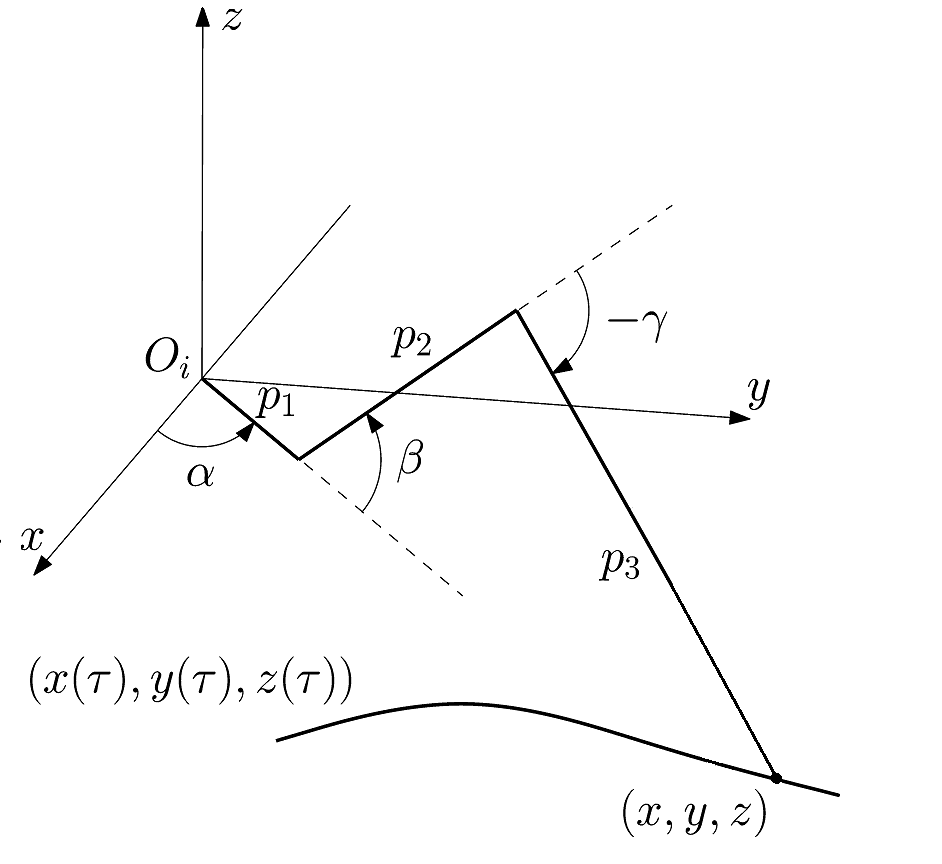
\includegraphics[width=75mm]{Introduction/leg1}\\}
\caption{Три степени свободы}
\label{fig1}
\end{figure}

\begin{figure}[ht]
\center{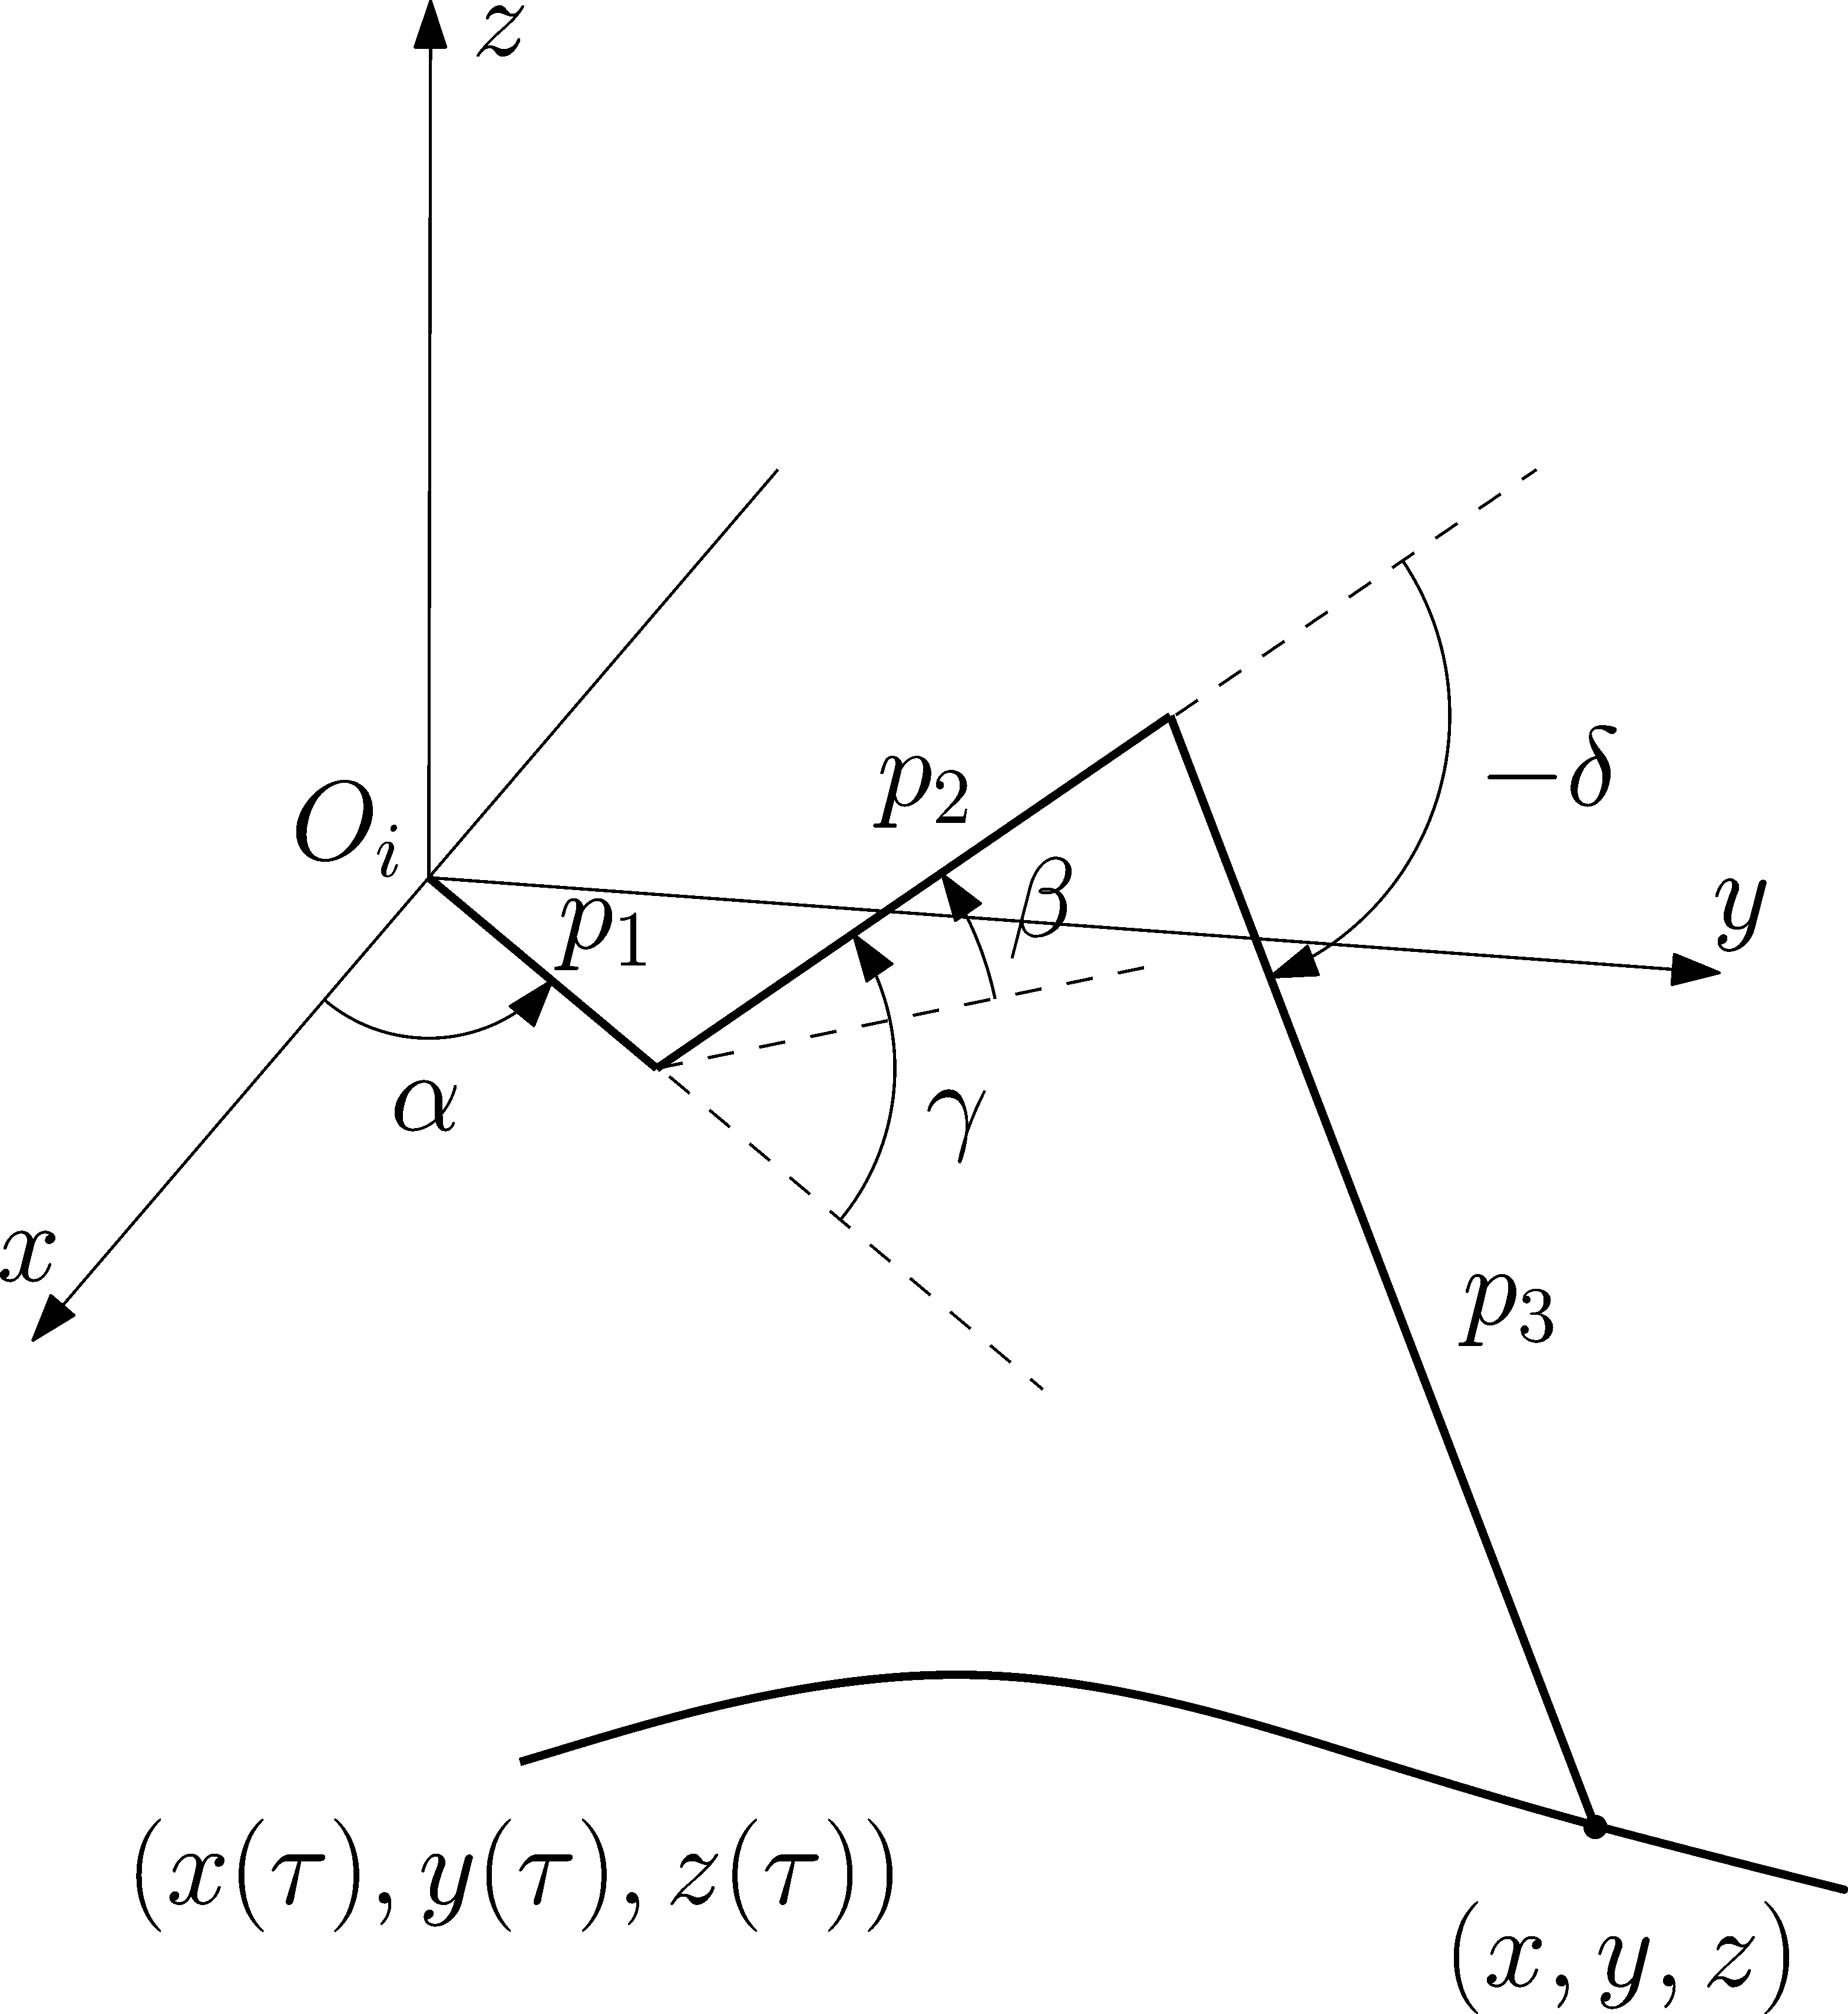
\includegraphics[width=75mm]{Introduction/leg4}\\}
\caption{Четыре степени свободы}
\label{fig2}
\end{figure}

Инсектоморфная нога с одной дополнительной степенью свободы (всего их становится четыре) приведена на рис.\ref{fig2}. В схему ноги добавлен вращательный шарнир позволяющий поворачивать плоскость ноги вокруг звена длины $p_1$. Пара соседних ног с такой подвижностью может быть использована в качестве манипулятора\cite{Langosz2013,Roennau2013} и позволит роботу захватывать объекты, в то время как оставшиеся четыре ноги обеспечат роботу необходимую устойчивость.

\begin{figure}[ht]
\center{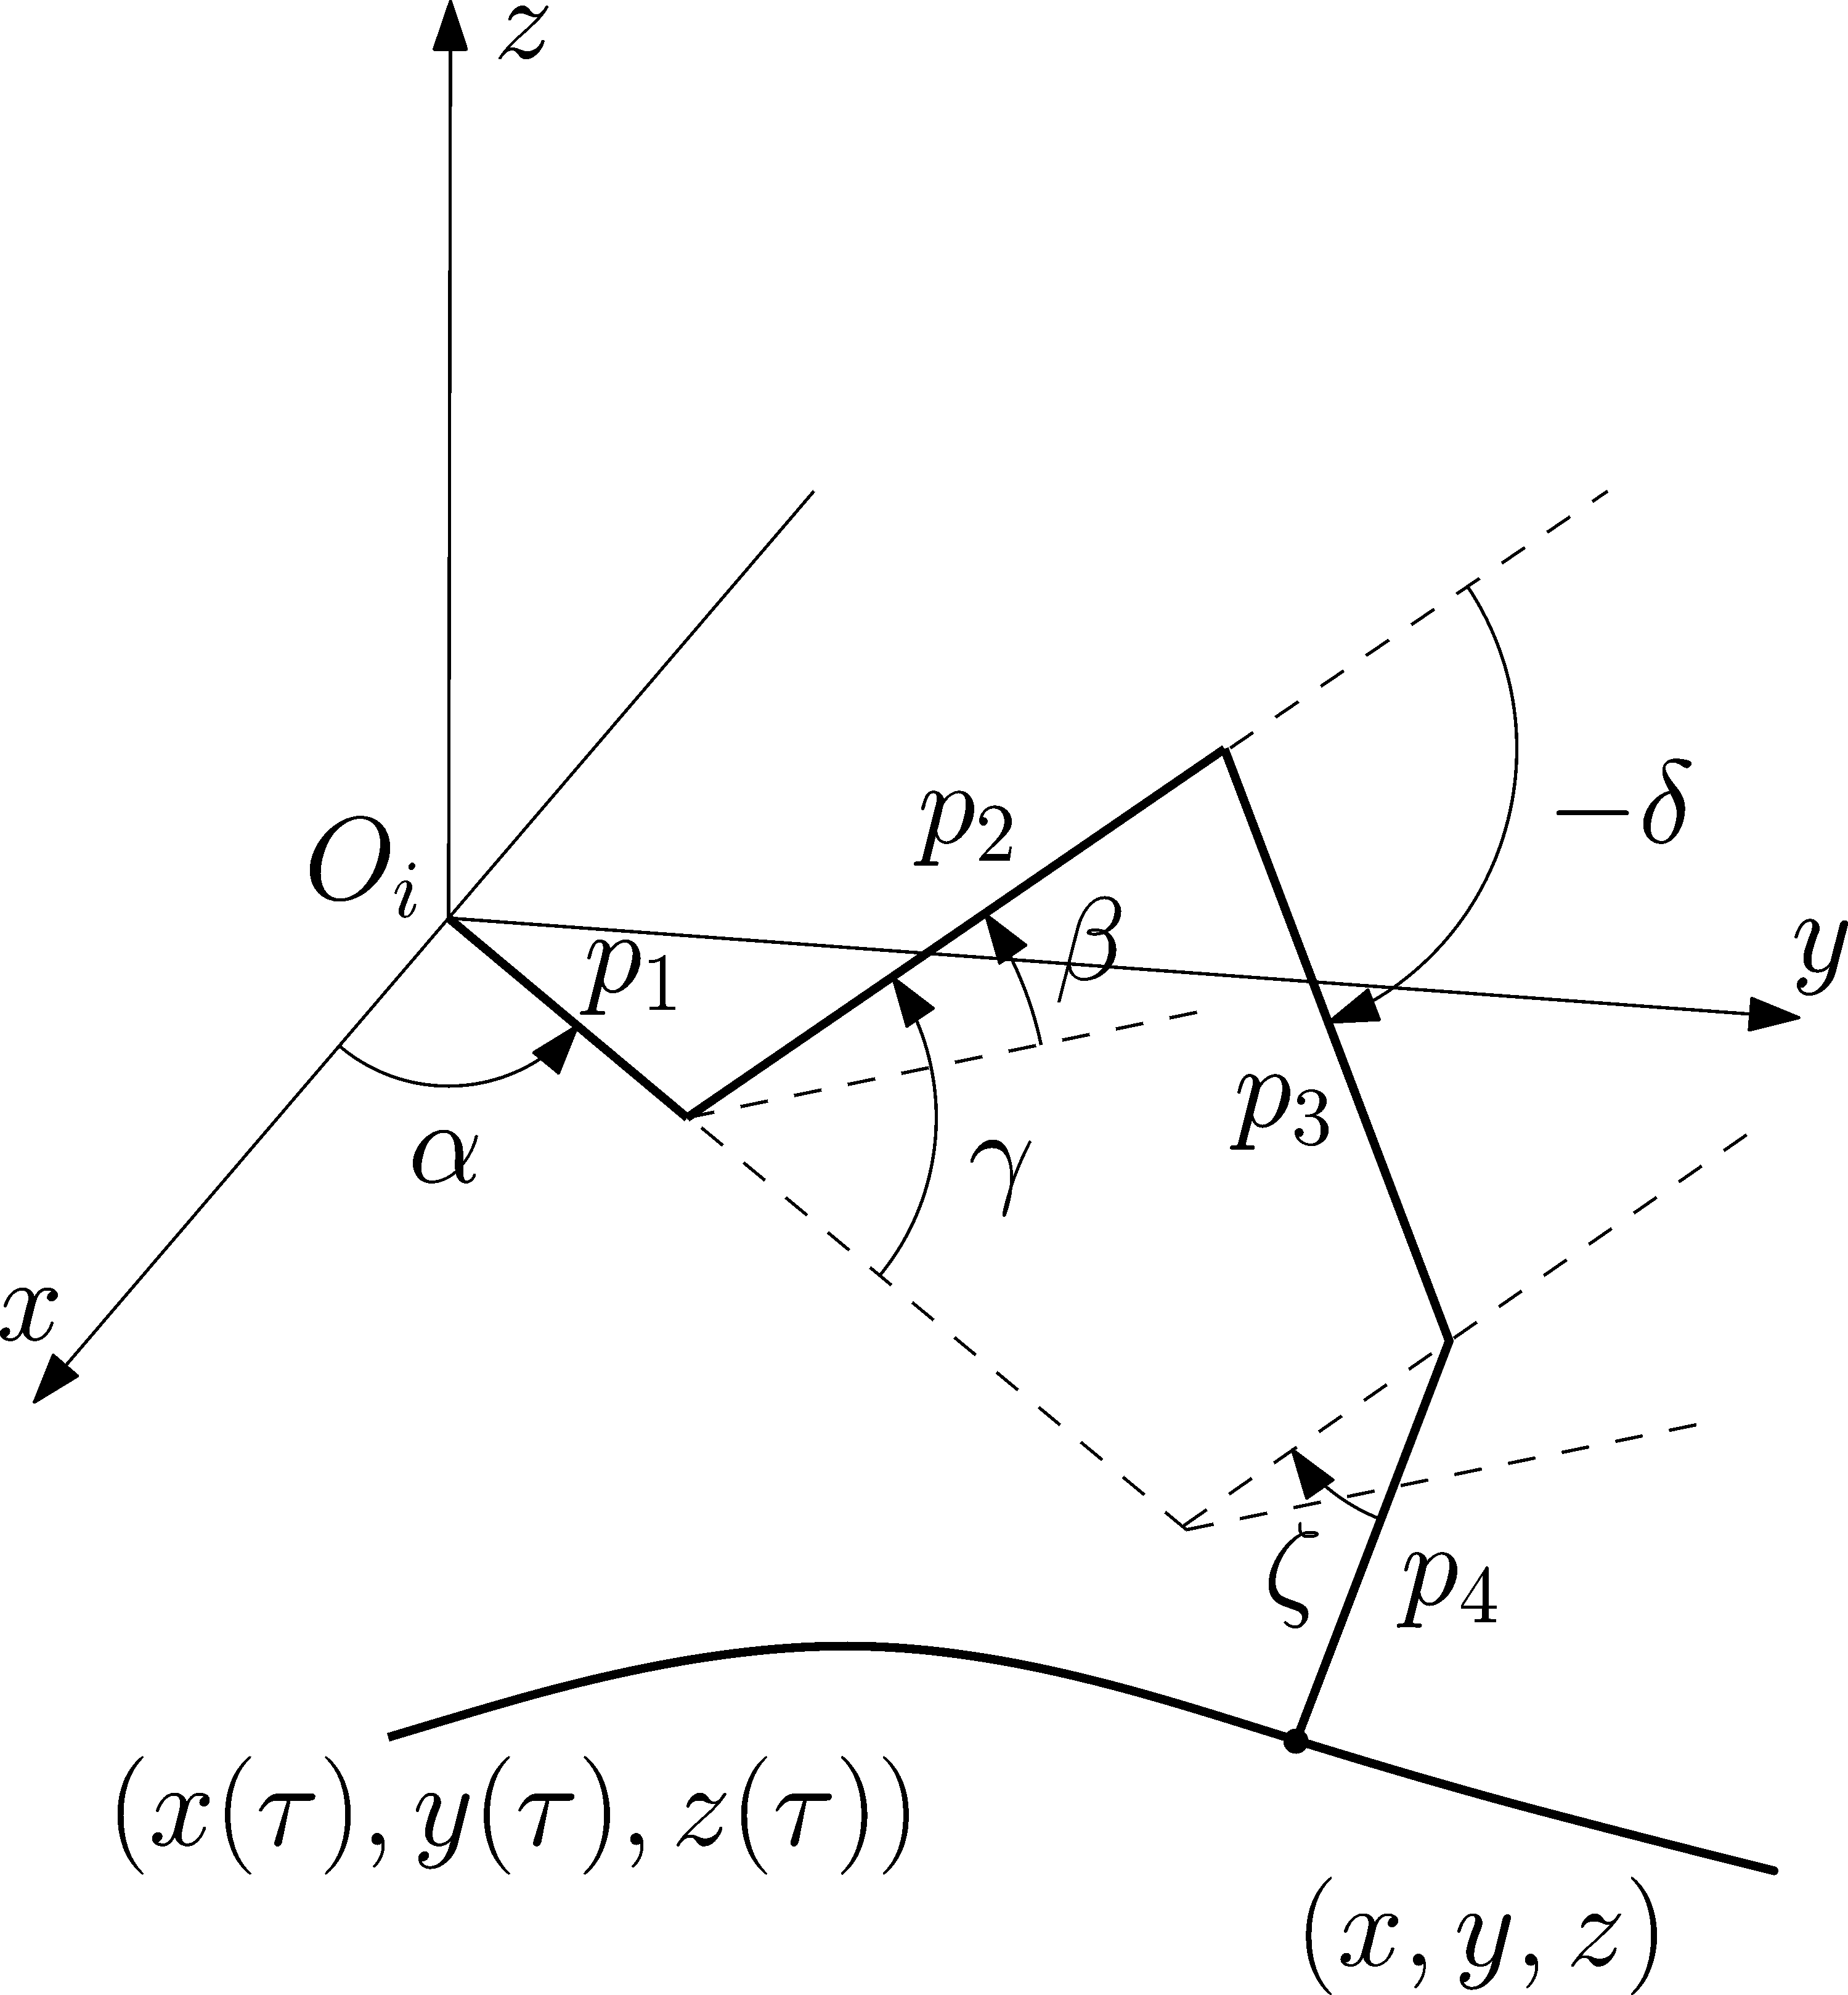
\includegraphics[width=75mm]{Introduction/leg5}\\}
\caption{Пять степеней свободы}
\label{fig3}
\end{figure} 

Инсектоморфная нога с двумя дополнительными степенями свободы приведена на рис.\ref{fig3}. Помимо дополнительного угла поворота плоскости ноги, в схеме имеется дополнительное звено на конце ноги. Угол поворота плоскости ноги и дополнительное звено позволят роботу ориентировать конец ноги под любым углом к контактной поверхности. Это может быть полезно в задачах по преодолению аппаратом различных препятствий и в задачах по манипуляции объектами сложной формы.

\begin{figure}
\begin{minipage}{0.49\linewidth}
\center{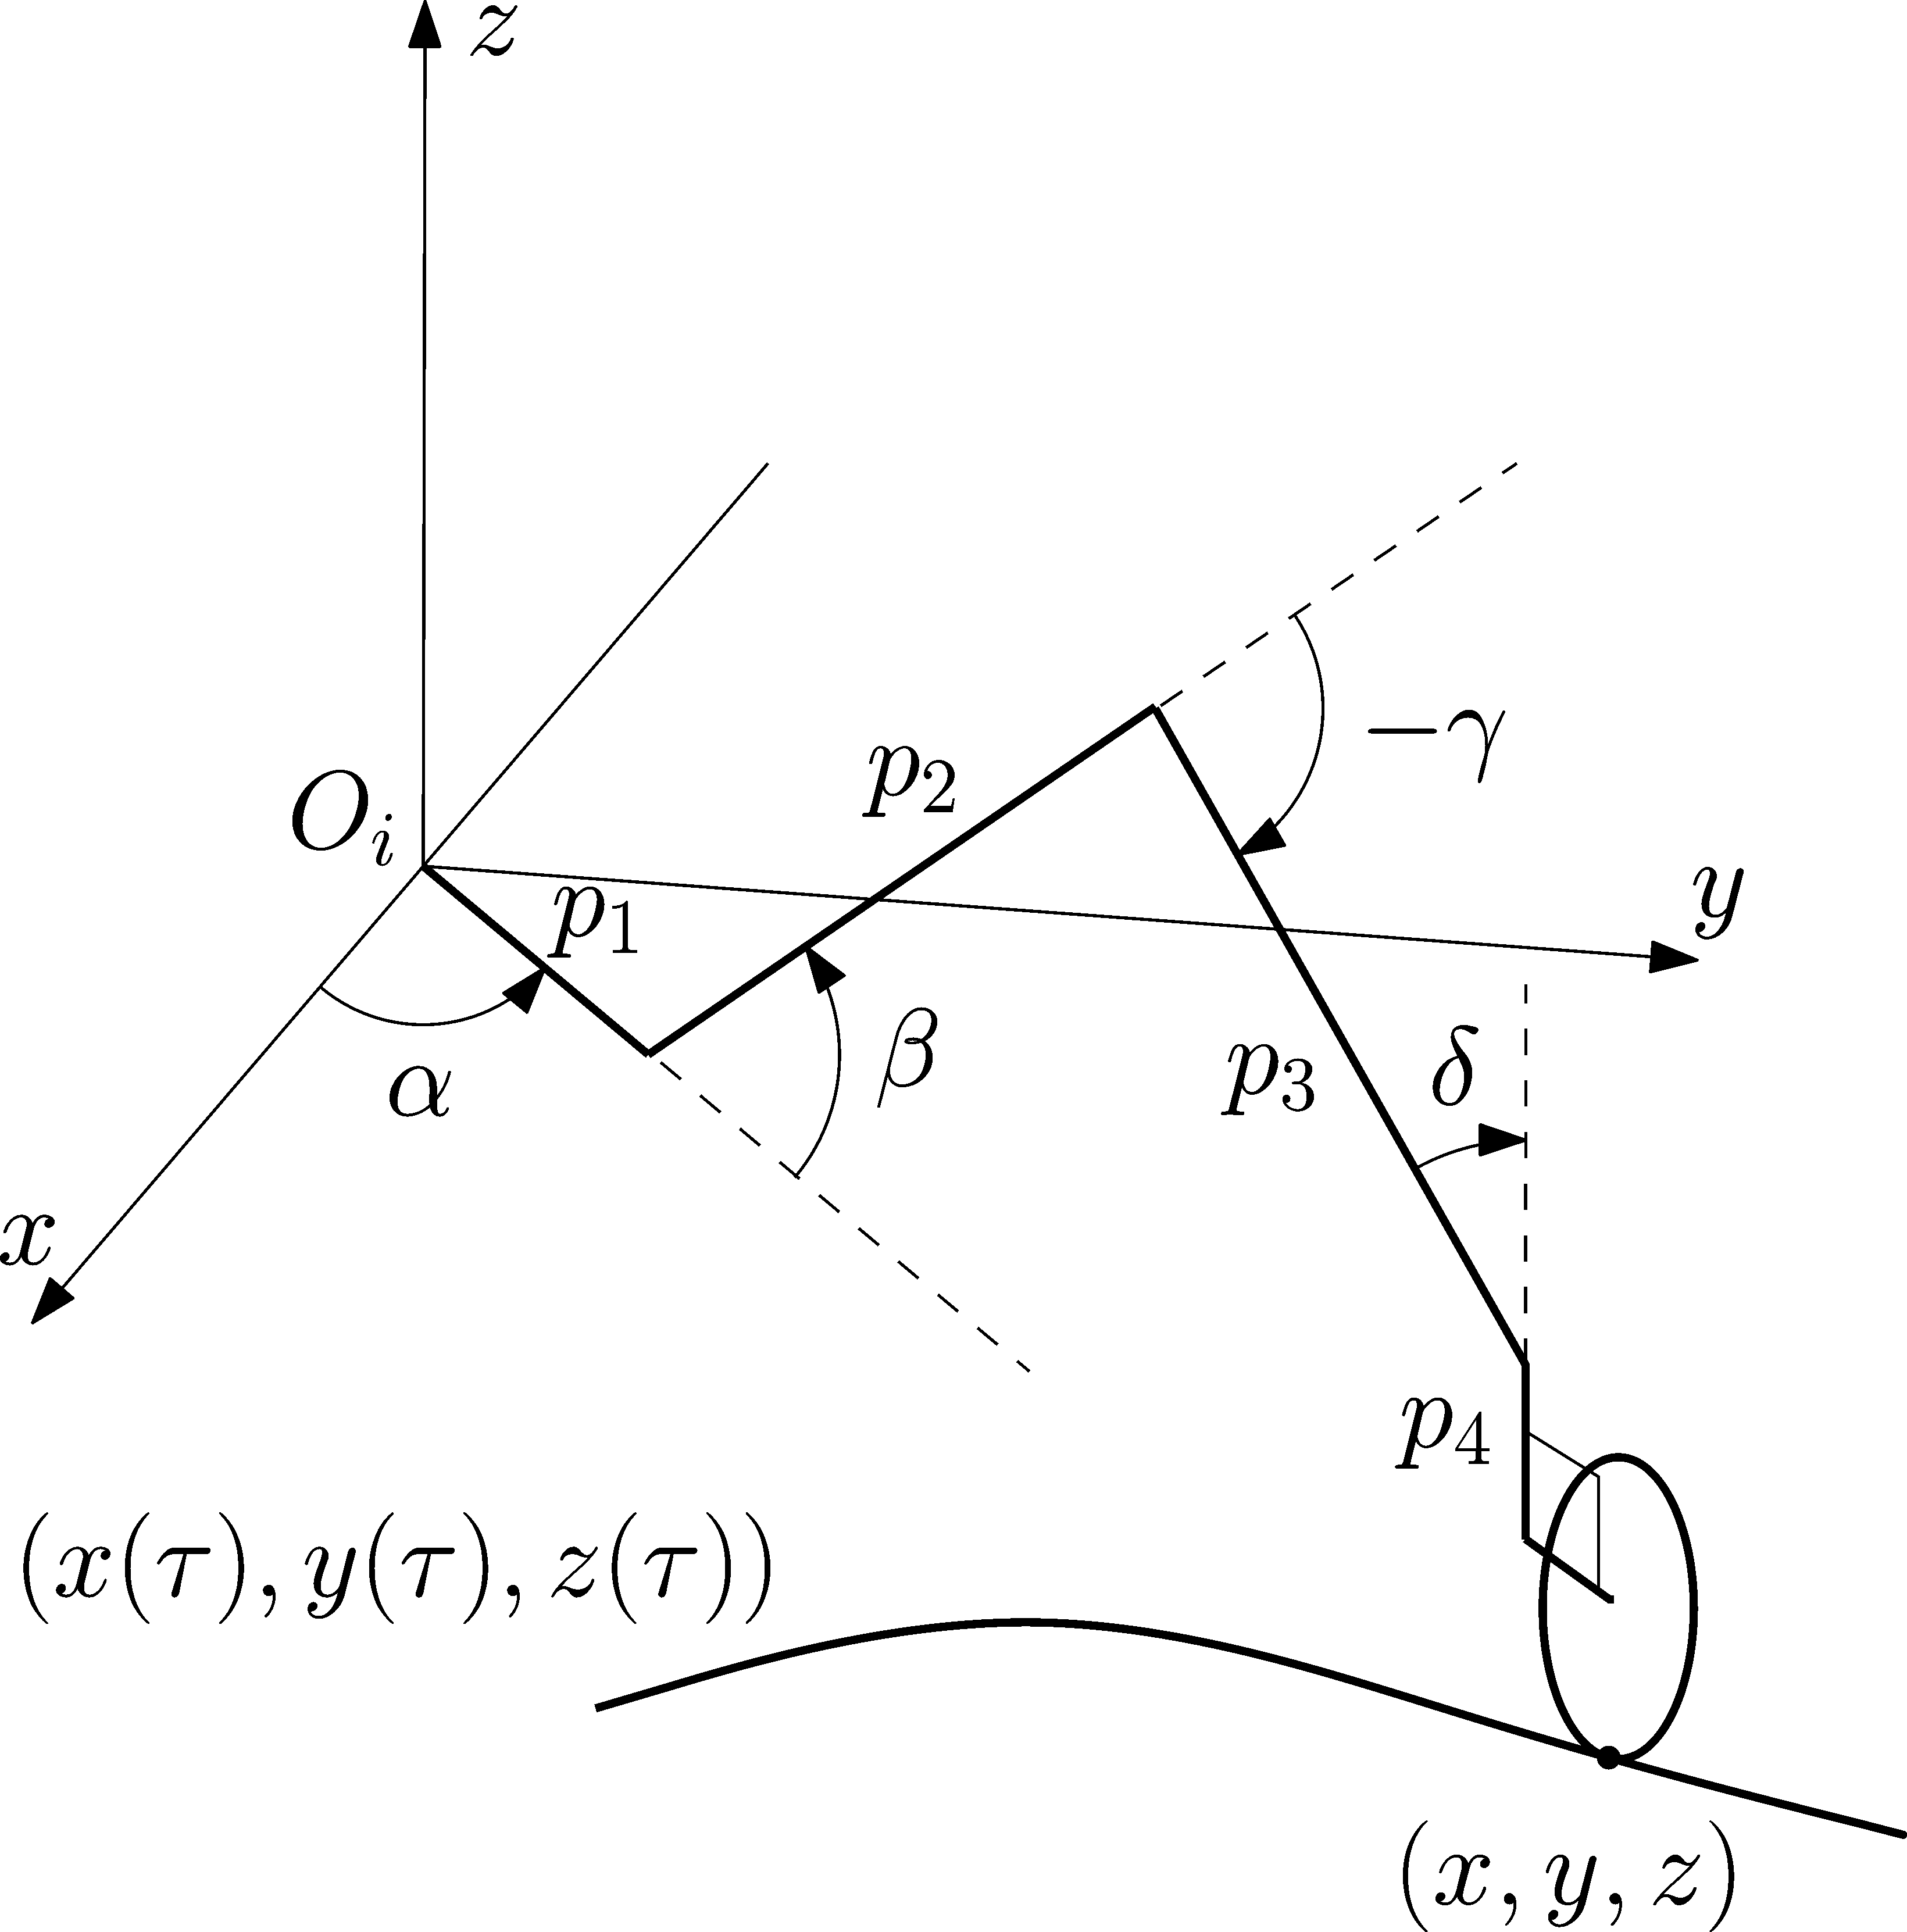
\includegraphics[width=75mm]{Introduction/leg2}\\ 1)}
\end{minipage}
\begin{minipage}{0.49\linewidth}
\center{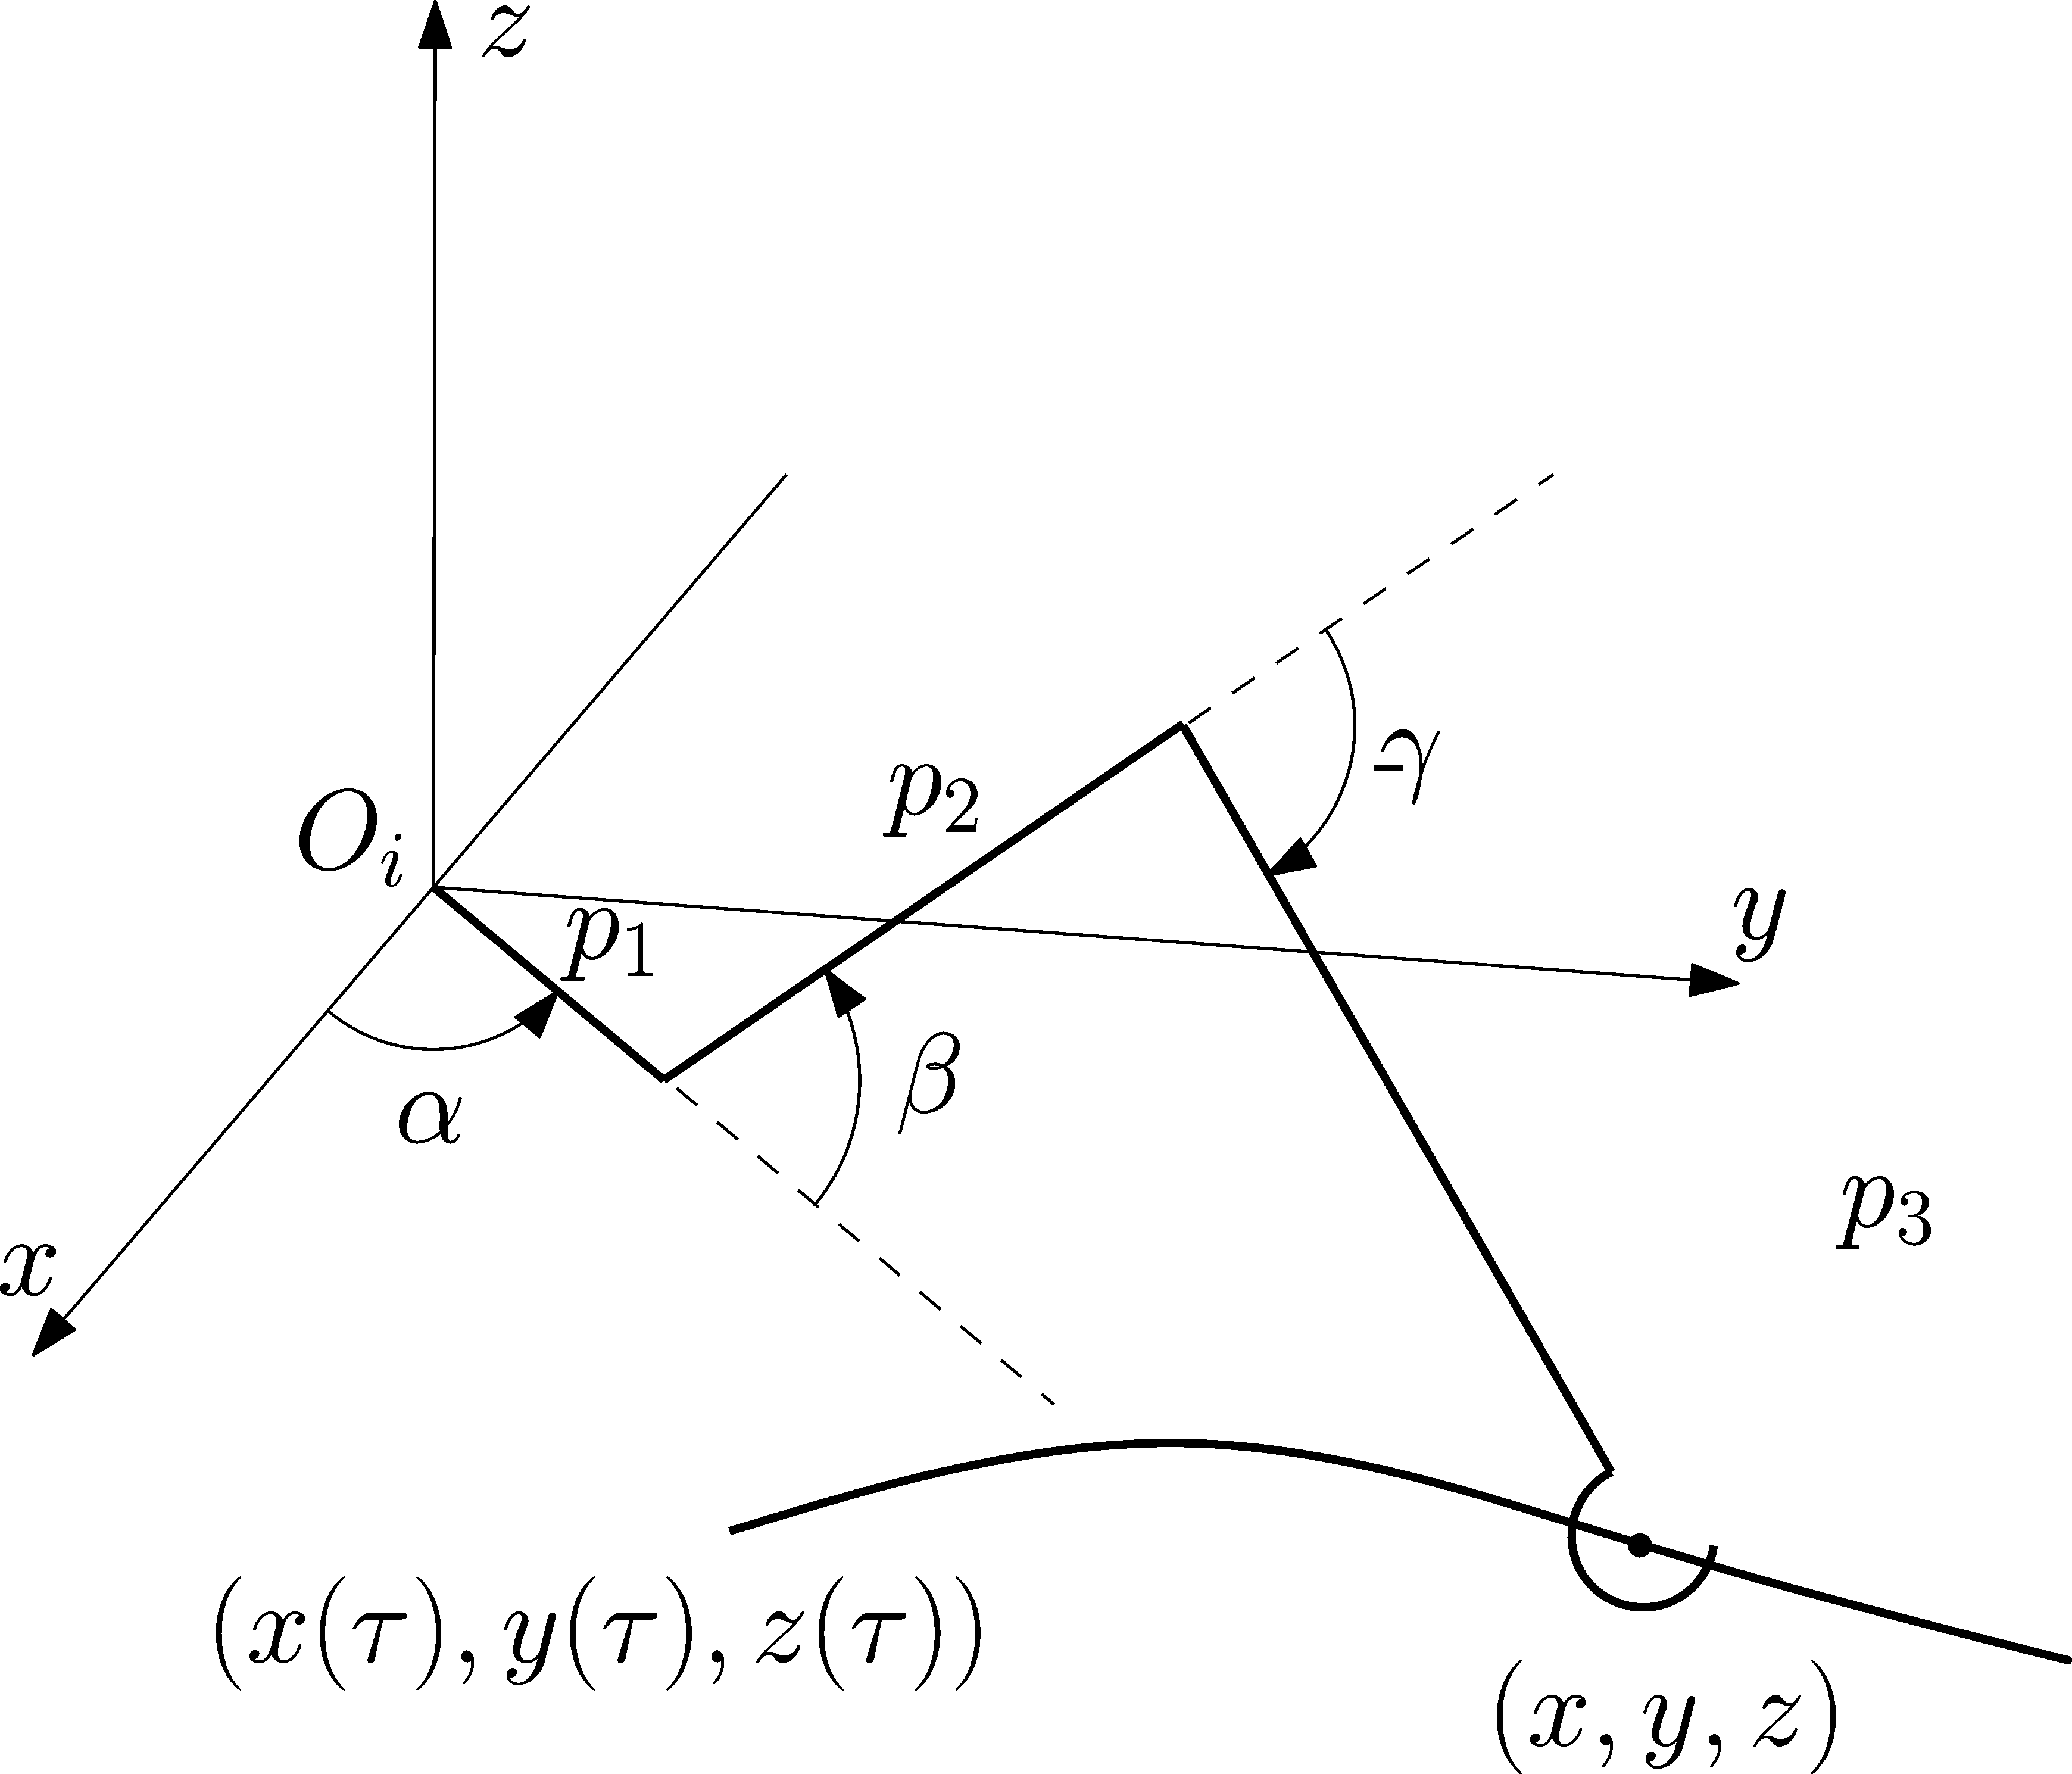
\includegraphics[width=75mm]{Introduction/leg3}\\2)}
\end{minipage}
\caption{Колесно-шагающая схема и схема с зацепляющим устройством}
\label{fig4}
\label{fig5}
\end{figure}

Колёсно-шагающая конструкция ноги (рис. \ref{fig4}) позволяет переключаться из обычного режима ходьбы в колёсный режим. Колёса могут быть как пассивными, т.е. свободно вращающимися, так и активными, например с электромоторами. В пассивном колёсном режиме движение может осуществляться за счёт волнообразного движения колёс относительно контактной поверхности. 

Наконец, схема ноги со специальным устройством зацепления на конце ноги, позволяющим аппарату закрепляться на вертикальных поверхностях, показана на рис. \ref{fig5}. При синтезе шагового цикла для такой ноги необходимо учитывать принцип работы зацепного механизма ноги.

Отметим, что с развитием микроэлектроники большое распространение получил класс небольших шагающих роботов, так называемых мини-гексаподов, т.е. небольших шестиногих роботов. Это класс небольших и лёгких роботов, собранных в основном, на основе модельных серводвигателей, широко используемых в радиоуправляемых моделях самолётов, автомобилей, катеров, вертолётов и т.д. Эти роботы могут быть частично или полностью автономными, могут нести на себе сложную систему сенсоров и датчиков, производить все необходимые вычисления и обработку показаний сенсоров на бортовом вычислительном устройстве. Их кинематические схемы в основном следуют базовой схеме на рис. \ref{fig1}

\clearpage

\section*{О конструкциях шагающих машин. Обзор.}
Попытки создания шагающих машин уходят в глубокую древность. Однако, многие первые разработки были попытками имитировать или копировать ходьбу четвероногих животных. В литературных источниках (например, в Википедии) имеются указания, что одна из наиболее древних разработок датирована 230 BC (230 год до Рождества Христова) - деревянная лошадь с повозкой, автор Лю Бань, Китай. Современные репродукции деревянной лошади показаны на рис. \ref{fig6}

\begin{figure}[h]
\begin{minipage}{0.49\linewidth}
\center{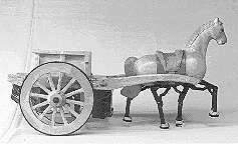
\includegraphics[width=80mm]{intro1}}
\end{minipage}
\hfill
\begin{minipage}{0.49\linewidth}
\center{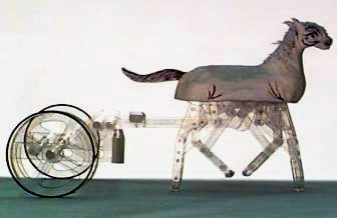
\includegraphics[width=80mm]{intro2}}
\end{minipage}
\caption{Схема одного из самых первых шагающих устройств}
\label{fig6}
\end{figure}

Разработки шагающих машин в дальнейшем прошли богатейшую историю. В современную историю одним из первых научной задачей анализа перемещения стопоходящих животных и устройств занялся известный русский математик и механик П.Л.Чебышев. Он в 1878 г. разработал образец так называемой стопоходящей машины \cite{..1945}, ее модель показана на рис. \ref{fig7}. Машина была построена на так называемых лямбда-механизмах Чебышева и была чисто механическим устройством. Стопоходящая машина является прекрасным примером его выдающихся работ по теории механизмов. 

\begin{figure}[here]
\center{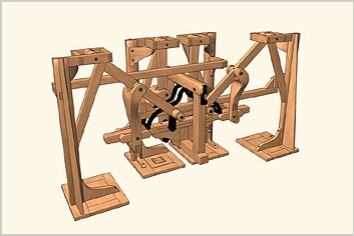
\includegraphics[width=90mm]{intro3}}
\caption{Стопоходящая машина П.Л.Чебышева}
\label{fig7}
\end{figure}

Машина Чебышева показала принципиальную возможность создания шагающего устройства современными средствами. Однако в современном мире подобные устройства реализуются как роботы, в которых значительная часть или все функции управления реализуются бортовой автоматической (компьютерной) системой. При этом уже не требуется механическая связь движущихся ног и других частей аппарата, их заменяет логическая связь этих элементов в программе управления.


Первые пионерские работы по шагающим роботам в СССР были начаты в ИМАШ АН СССР, а затем их возглавил и стал бессменным лидером и руководителем академик РАН Д.Е. Охоцимский в ИПМ АН СССР (позднее ИПМ им.М.В.Келдыша РАН). Эти работы были на уровне передовых западных исследований, а во многом их опережали \cite{1984,1982,1972a,1978,1971,1974,1972,1974d,1977,1986b}.
Примерно в одно и то же время - в период 1972-1975 гг. - были созданы первые макеты многоногих шагающих машин. На рис.\ref{fig8} показан макет шагающей машины, разработанный в Институте машиноведения Академии наук СССР.

\begin{figure}[here]
\center{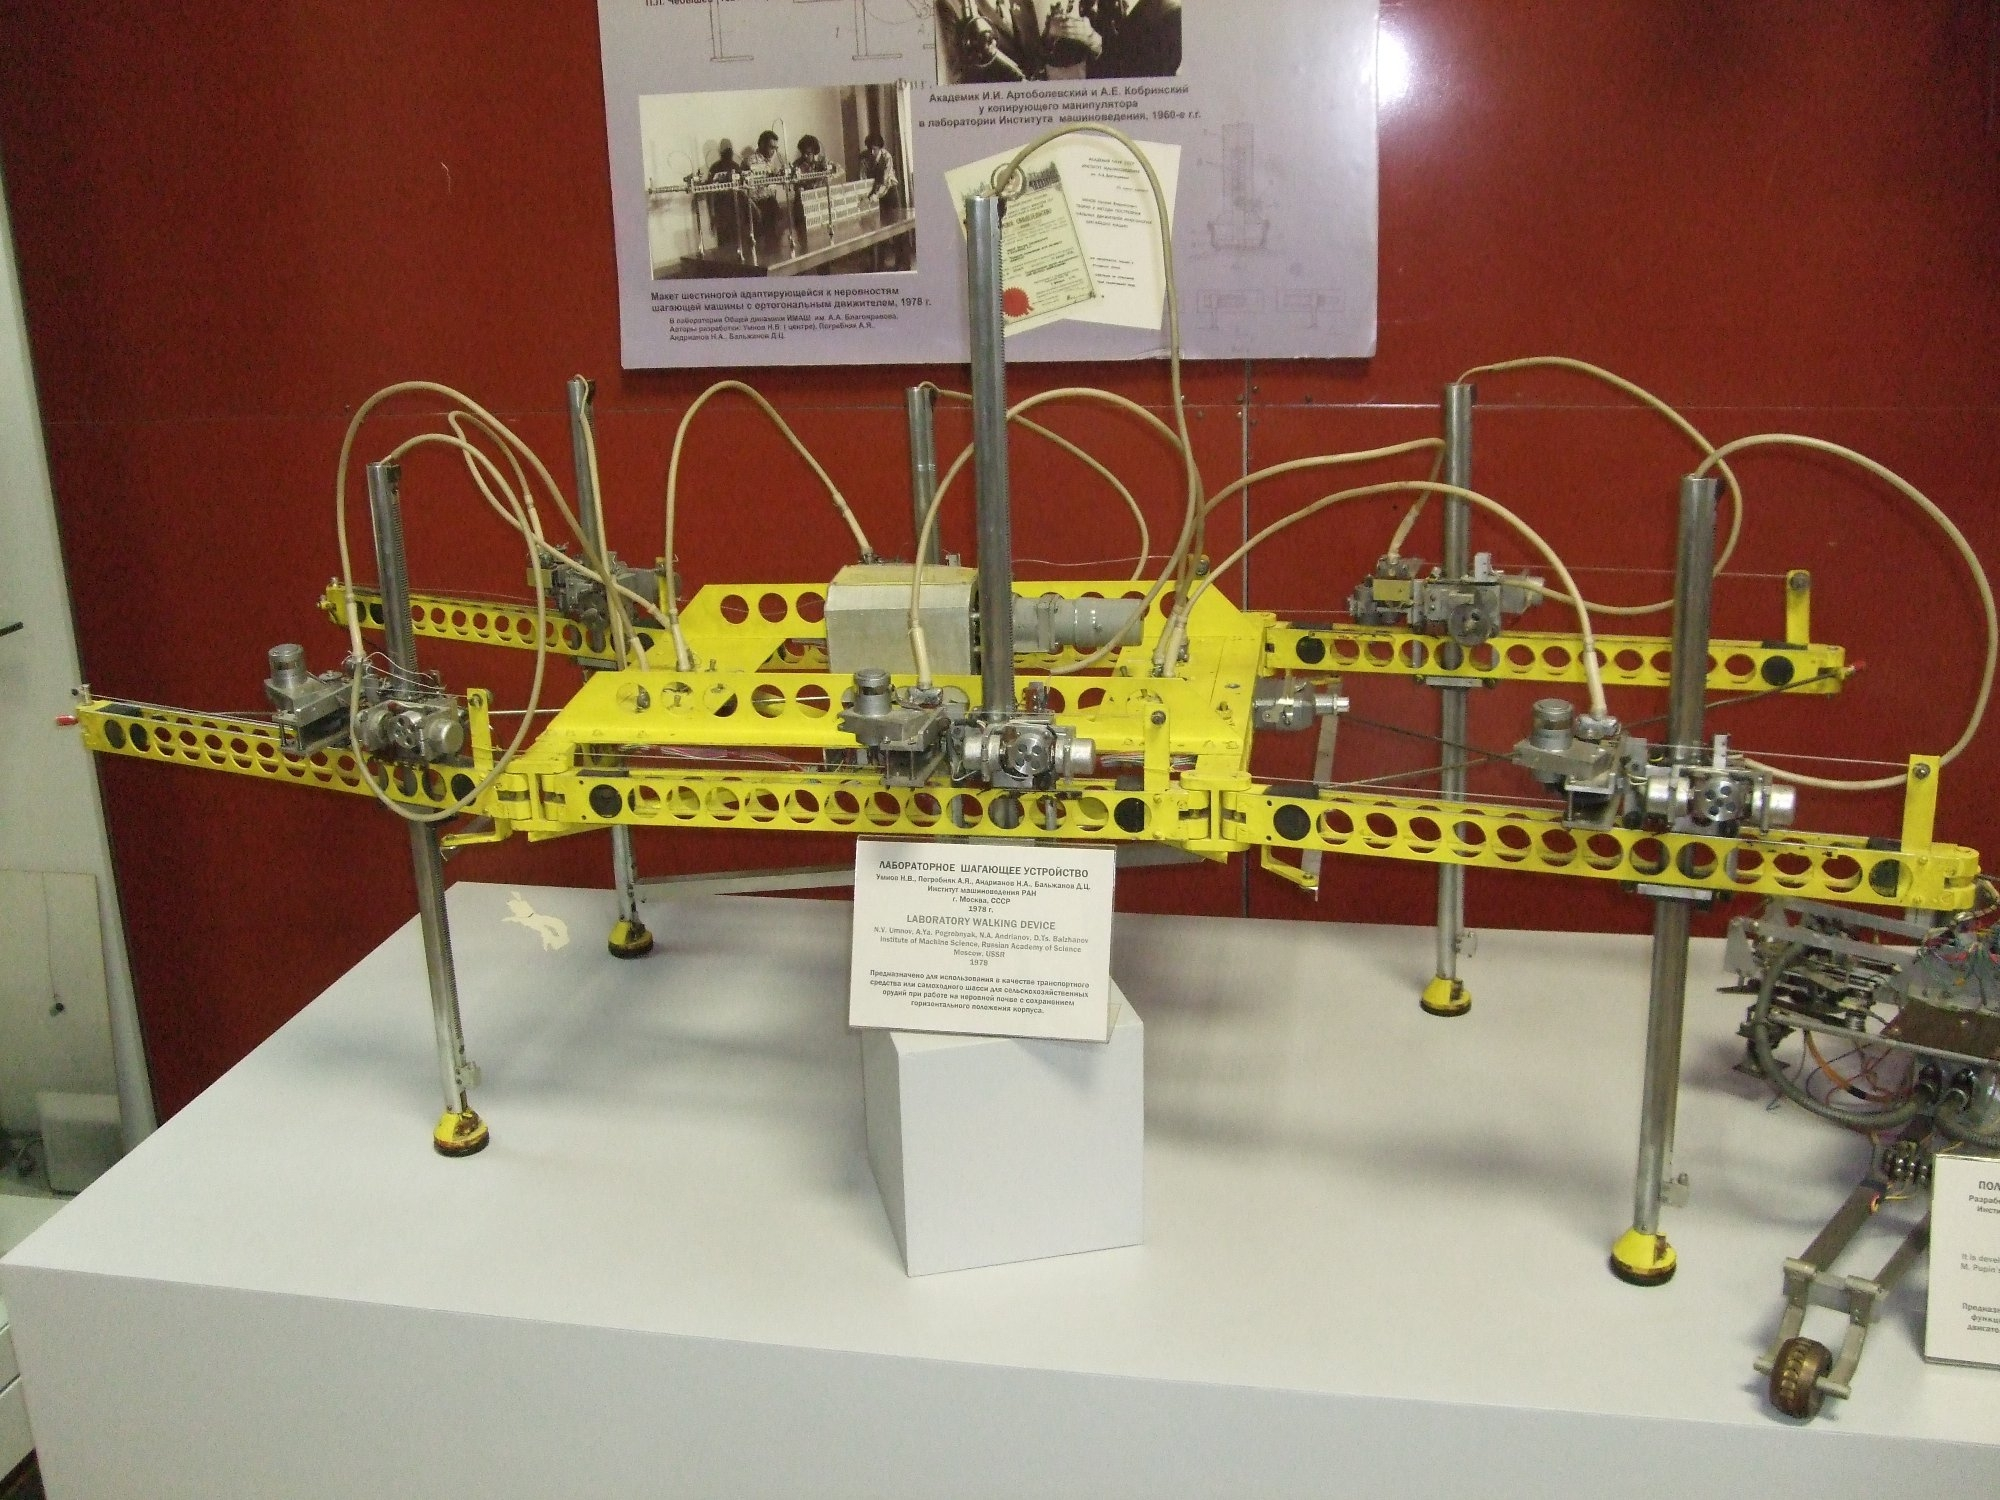
\includegraphics[width=90mm]{intro4}}
\caption{Шагающая машина ИМАШ РАН}
\label{fig8}
\end{figure}

В этой машине был использован оригинальный принцип организации ходьбы. Машина имеет 6 ног с так называемыми ортогональными приводами. Его преимущества состоят в более простых расчетных схемах синтеза движения ног и корпуса аппарата.
На рис.\ref{fig9} показаны макеты шестиногих шагающих машин, созданные в Институте прикладной математики АН СССР. Слева показан первый образец, созданный в содружестве ИПМ им. М.В.Келдыша АН СССР и Ленинградского механического института (ЛМИ), справа - второй образец, созданный несколько позднее при сотрудничестве ИПМ им. М.В.Келдыша АН СССР и Ленинградского института ВНИИТРАНСМАШ. 
Отметим, что эти аппараты имели так называемые инсектоморфные ноги, каждая из которых имела по три степени подвижности (три степени свободы). На рис.\ref{fig9} оба аппарата показаны в варианте с оснащением лазерным дальномерным устройством - Лазерным Измерителем Расстояний ЛИР. С помощью ЛИР роботы осматривали поверхность передвижения, и затем, управляющая роботами ЭВМ принимала решения о движении. Наличие шести ног позволяло решить принципиальную задачу устойчивости движения робота - робот мог передвигаться статически устойчивой походкой, если в каждый момент времени в опоре находилось не менее трех ног. Именно это обстоятельство определило интерес к многоногим машинам.

\begin{figure}[here]
\begin{minipage}{0.49\linewidth}
\center{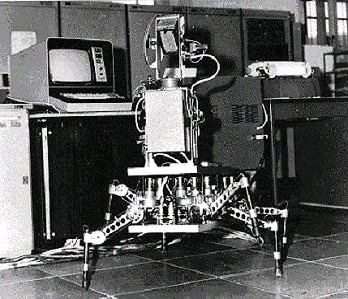
\includegraphics[width=70mm]{intro5}}
\end{minipage}
\hfill
\begin{minipage}{0.49\linewidth}
\center{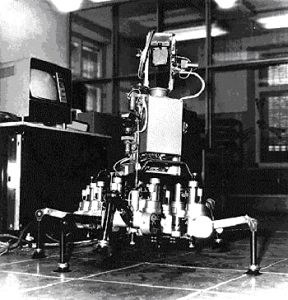
\includegraphics[width=70mm]{intro6}}
\end{minipage}
\caption{Шагающие роботы ИПМ им. М.В.Келдыша АН СССР. Фото 1975 г}
\label{fig9}
\end{figure} 

Позднее на базе этих разработок совместно ИПМ им. М.В.Келдыша АН СССР и ВНИИТРАНСМАШ в 1975 г. был создан большой натурный макет шестиногой машины НМША (Натурный Макет Шагающего Аппарата), которая была способна нести человека-оператора (водителя). Масса машины 750 кг. Скорость движения 0,7 км/ч, грузоподъёмность 50 кг, дорожный просвет 1,5 м. Машина показана на фотографиях на рис.\ref{fig10}.

\begin{figure}[h]
\begin{minipage}{0.49\linewidth}
\center{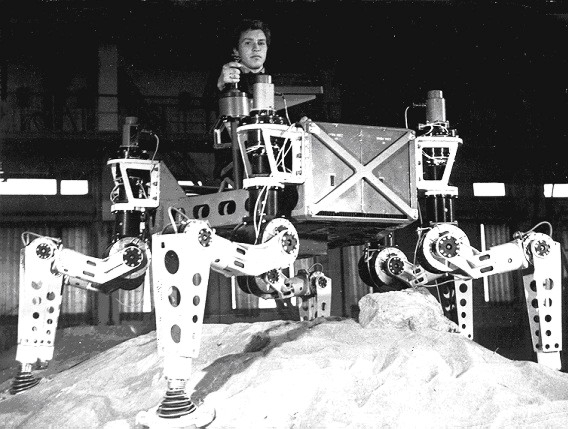
\includegraphics[width=70mm]{intro7}}
\end{minipage}
\hfill
\begin{minipage}{0.49\linewidth}
\center{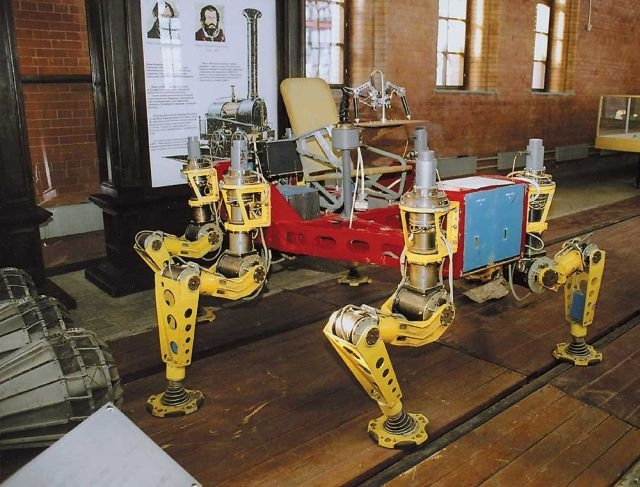
\includegraphics[width=70mm]{intro8}}
\end{minipage}
\caption{Аппарат НМША}
\label{fig10}
\end{figure} 

Указанные исследования продолжаются в настоящее время, на рис.\ref{fig11} показан третий макет робота, создаваемый как модификация предыдущих в ИПМ им.М.В.Келдыша РАН. На роботе реализована оригинальная бортовая микропроцессорная система управления, построенная как бортовая микрокомпьютерная управляющая сеть. Робот оснащен необходимым набором сенсоров.

\begin{figure}[here]
\begin{minipage}{0.49\linewidth}
\center{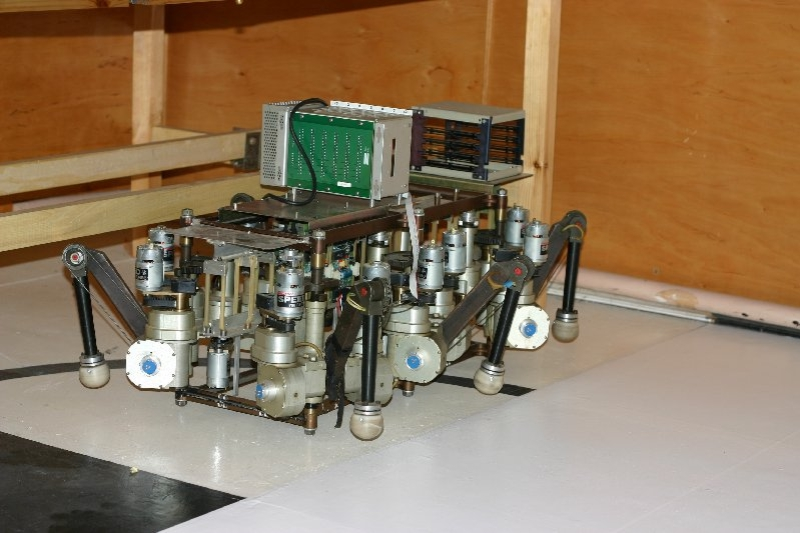
\includegraphics[width=80mm]{intro9}}
\end{minipage}
\hfill
\begin{minipage}{0.49\linewidth}
\center{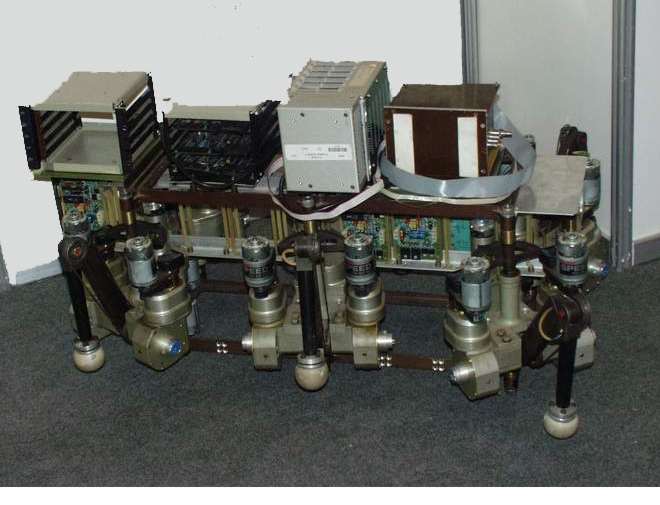
\includegraphics[width=80mm]{intro10}}
\end{minipage}
\caption{Шагающий робот ИПМ им. М.В.Келдыша РАН. 
Фотографии 2009 г}
\label{fig11}
\end{figure}
 
Работы по исследованию шестиногих аппаратов продолжаются и в МГУ, в Институте Механики. Они ведутся на основе модернизации самого первого проекта этого института, в котором создавался робот МАША (МАшина ШАгающая). 

\begin{figure}[here]
\begin{minipage}{0.49\linewidth}
\center{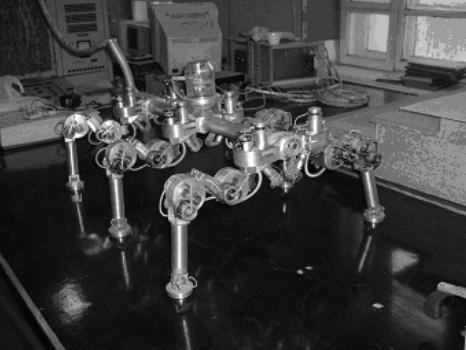
\includegraphics[width=80mm]{intro11}}
\end{minipage}
\hfill
\begin{minipage}{0.49\linewidth}
\center{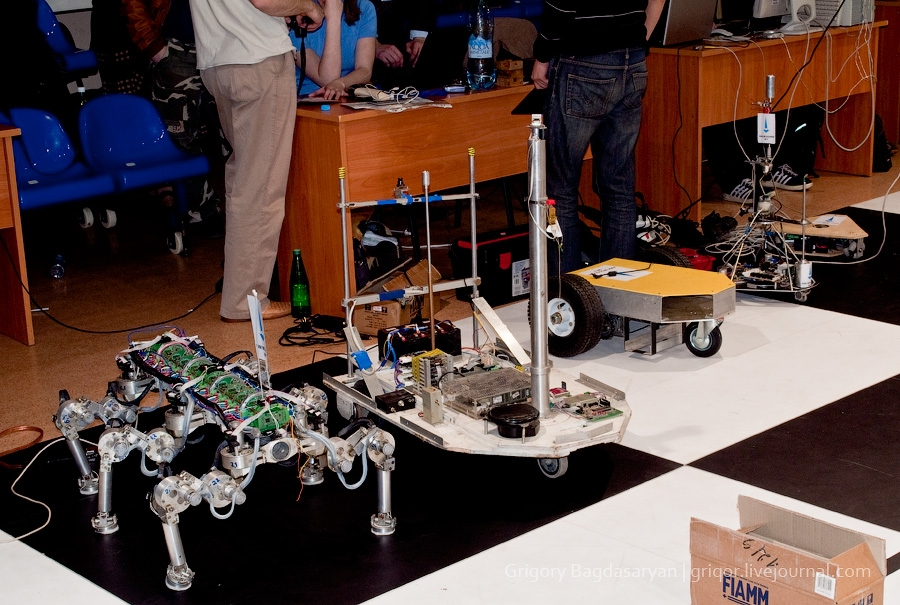
\includegraphics[width=80mm]{intro12}}
\end{minipage}
\caption{Робот Института Механики МГУ. Первая (1975 г.) и современная версии}
\label{fig12}
\end{figure}
 
На рис.\ref{fig12} показана первая (слева) и современная (справа) версии робота МАША, на второй фотографии аппарат показан на переднем плане - на Фестивале мобильных роботов в МГУ. Робот также имеет шесть инсектоморфных ног и снабжен необходимым набором сенсоров.

Далее нужно отметить, что проекты шагающих машин выполнены практически во всех технологически развитых странах, - США, Японии, Англии, Финляндии, Бельгии, Германии, Испании, и других странах. Перечислим некоторые примеры. 

На рис.\ref{fig13} приведена одна из первых разработок в США. Авторы –Robert McGhee и Andrew Frank. Разработка была хорошо известна и получила в научно-популярной прессе шутливые прозвища Phoney Poney или ''Калифорнийская лошадь''.

\begin{figure}[h]
\center{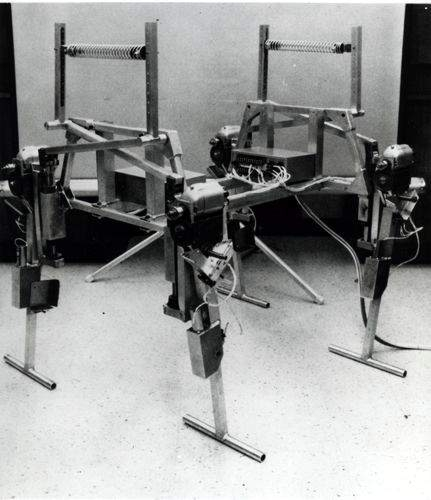
\includegraphics[width=80mm]{intro13}}
\caption{1968 г. Phoney Poney. Калифорнийская лошадь}
\label{fig13}
\end{figure}

\begin{figure}[h]
\center{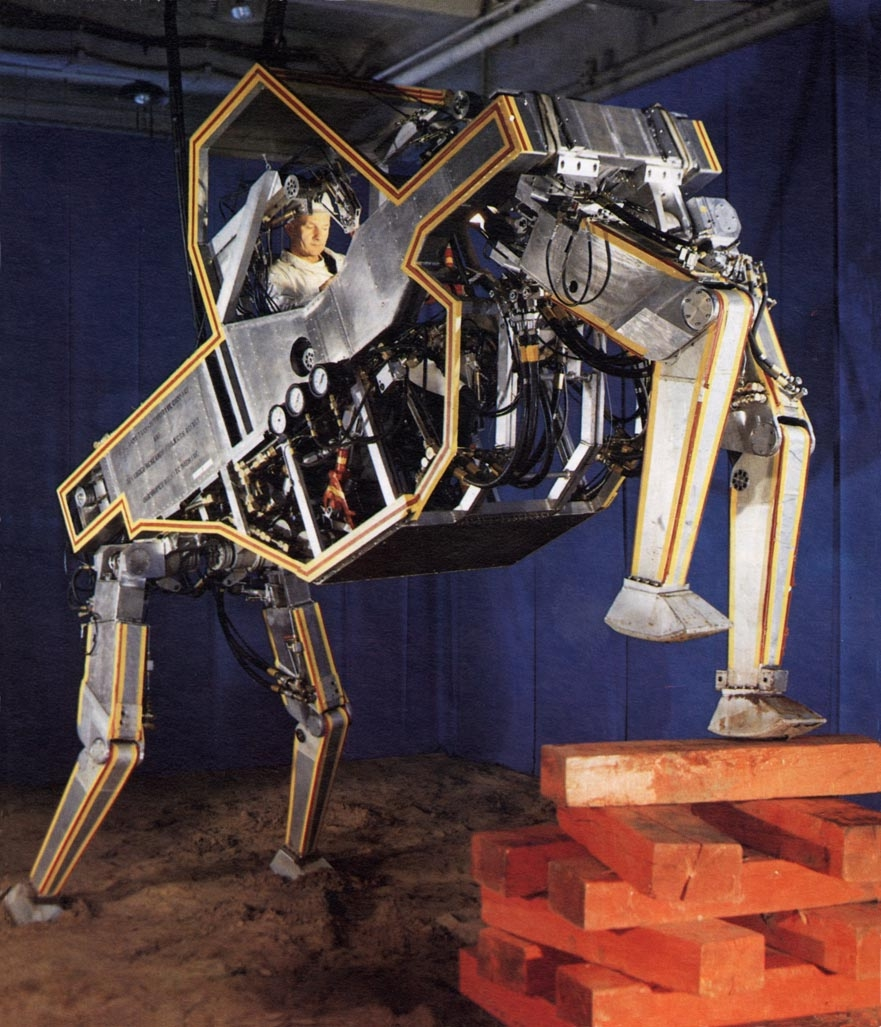
\includegraphics[width=80mm]{intro14}}
\caption{1969 г. GE Walking Truck. Ralph Mosher. США}
\label{fig14}
\end{figure}

На рис.\ref{fig14} - тяжелая шагающая машина General Electric, США. Управление ею было построено на основе копирующих автоматов, но человек, ведущий ее и руками и ногами, выдерживал всего порядка десяти минут. Такой сложной была система управления, требующая огромного напряжения внимания и сил. По этим результатам был сделан однозначный вывод: управление аппаратом необходимо переложить на компьютер. Все последующие аппараты строились как роботы с компьютерным управлением, реализующим больший или меньший объем функций управления в супервизорном или автономном режимах.

На последующих фотографиях на рис.\ref{fig15}- \ref{fig16} - разработки 70-80 годов ХХ века, затем более поздние и современные аппараты зарубежных лабораторий и фирм.

На рис.\ref{fig17} показана концепт-машина, созданная в Финляндии в фирме Plustech Oy Ltd. Машина предназначена для работы в лесу на лесоразработках, в условиях труднопроходимой местности с валунами, где не проходит тяжелая колесная и гусеничная техника.

\begin{figure}
\center{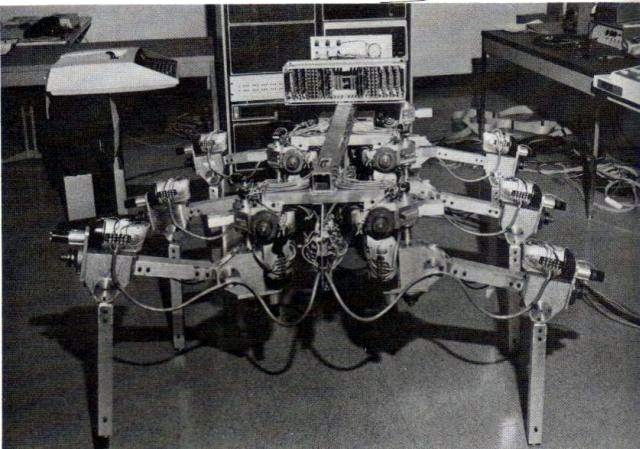
\includegraphics[width=90mm]{intro15}}
\caption{1976 г. Средний шестиногий робот. Университет Огайо. 
профессор R. McGhee. США}
\label{fig15}
\end{figure}

\begin{figure}
\begin{minipage}{0.49\linewidth}
\center{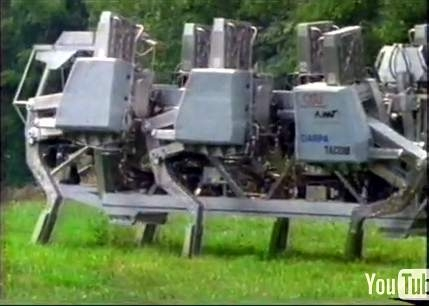
\includegraphics[width=80mm]{intro16}}
\end{minipage}
\hfill
\begin{minipage}{0.49\linewidth}
\center{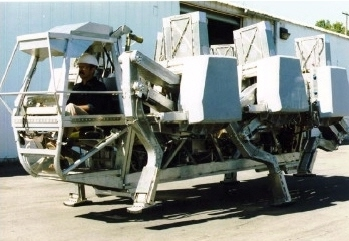
\includegraphics[width=80mm]{intro17}}
\end{minipage}
\caption{1984 – 1991 гг. ASV. Тяжелый шестиногий аппарат. 
Университет Огайо, Стенфордский университет. США.
Руководитель разработки профессор K.J.Waldron}
\label{fig16}
\end{figure}



\begin{figure}[here]
\center{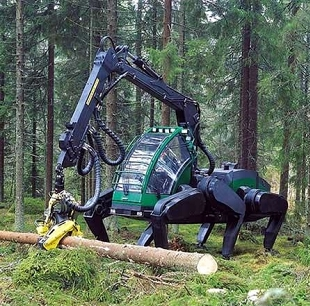
\includegraphics[width=90mm]{intro18}}
\caption{Plustech Oy Ltd. Финляндия, 1999}
\label{fig17}
\end{figure}

Далее – японские разработки (рис. \ref{fig18},\ref{fig19}), роботы семейства Titan. Масса робота Titan 11 составляет 7 тонн.

\begin{figure}[here]
\begin{minipage}{0.49\linewidth}
\center{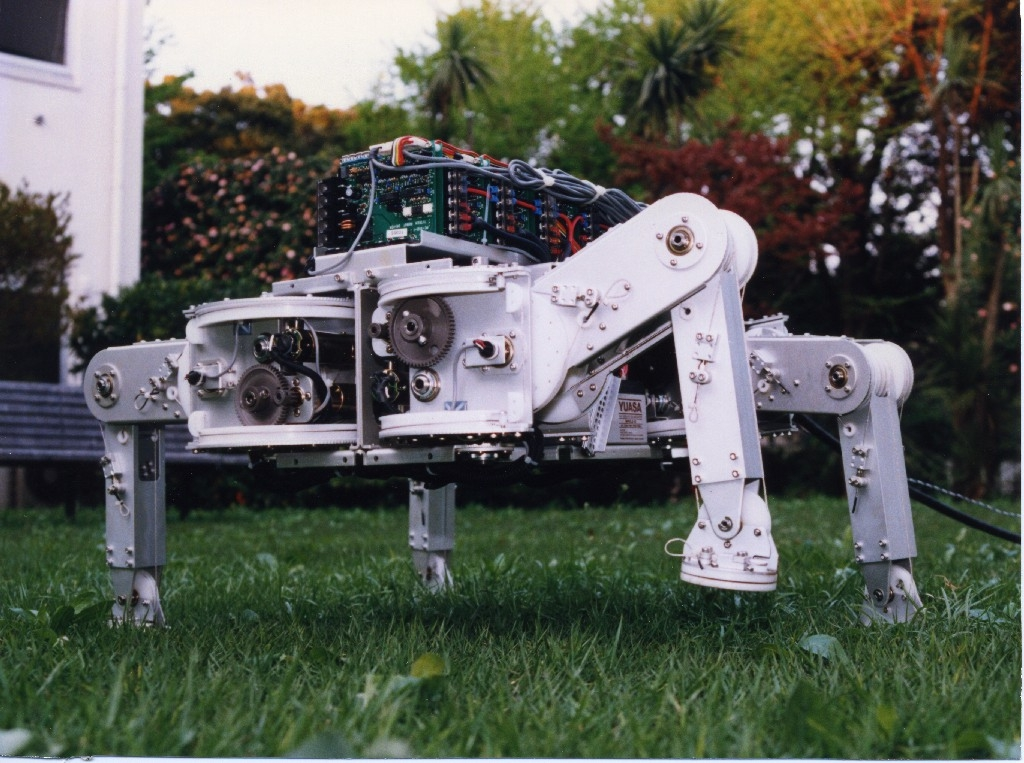
\includegraphics[width=80mm]{intro19}}
\end{minipage}
\hfill
\begin{minipage}{0.49\linewidth}
\center{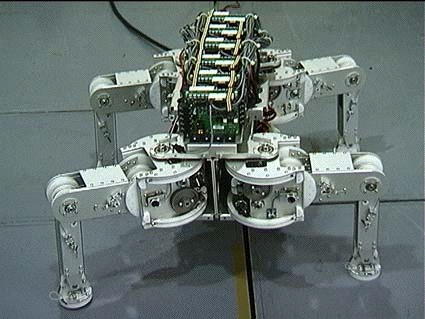
\includegraphics[width=80mm]{intro20}}
\end{minipage}
\caption{Titan 8. Япония. Лаборатория профессора Хиросе}
\label{fig18}
\end{figure}

\begin{figure}[here]
\center{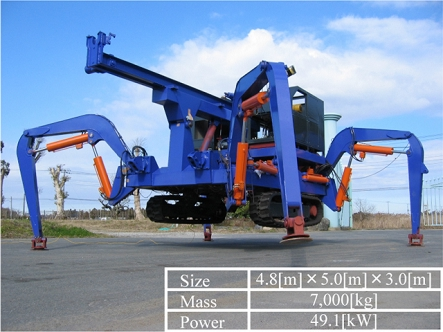
\includegraphics[width=90mm]{intro21}}
\caption{Titan 11. Япония. Лаборатория профессора Хиросе}
\label{fig19}
\end{figure}

На рис.\ref{fig20} и рис.\ref{fig21} – разработки Германии и Испании, семейства средних роботов Lauron и Silo.

\begin{figure}[here]
\begin{minipage}{0.49\linewidth}
\center{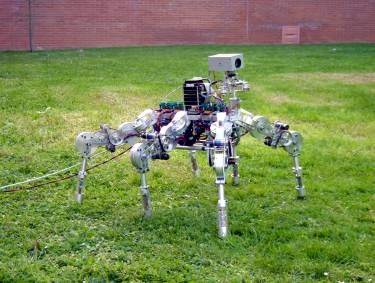
\includegraphics[width=80mm]{intro22}}
\end{minipage}
\hfill
\begin{minipage}{0.49\linewidth}
\center{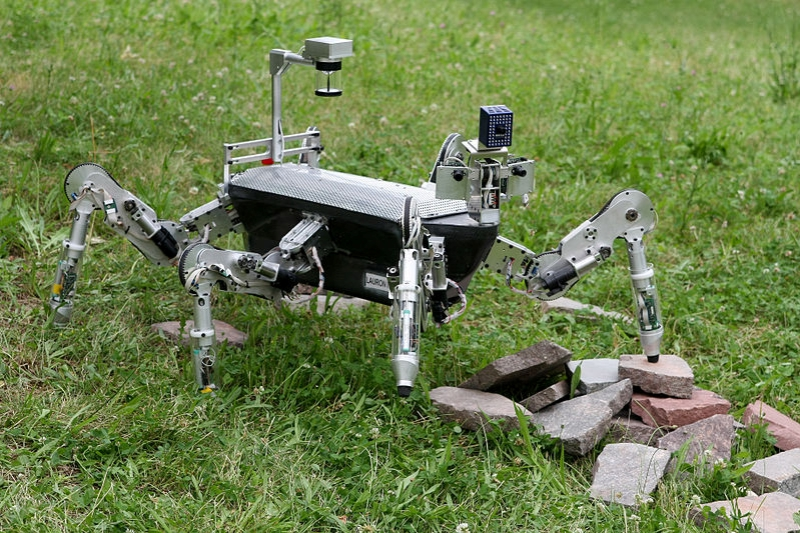
\includegraphics[width=80mm]{intro23}}
\end{minipage}
\caption{Lauron 3, Lauron 4. Германия}
\label{fig20}
\end{figure} 

\begin{figure}[here]
\begin{minipage}{0.49\linewidth}
\center{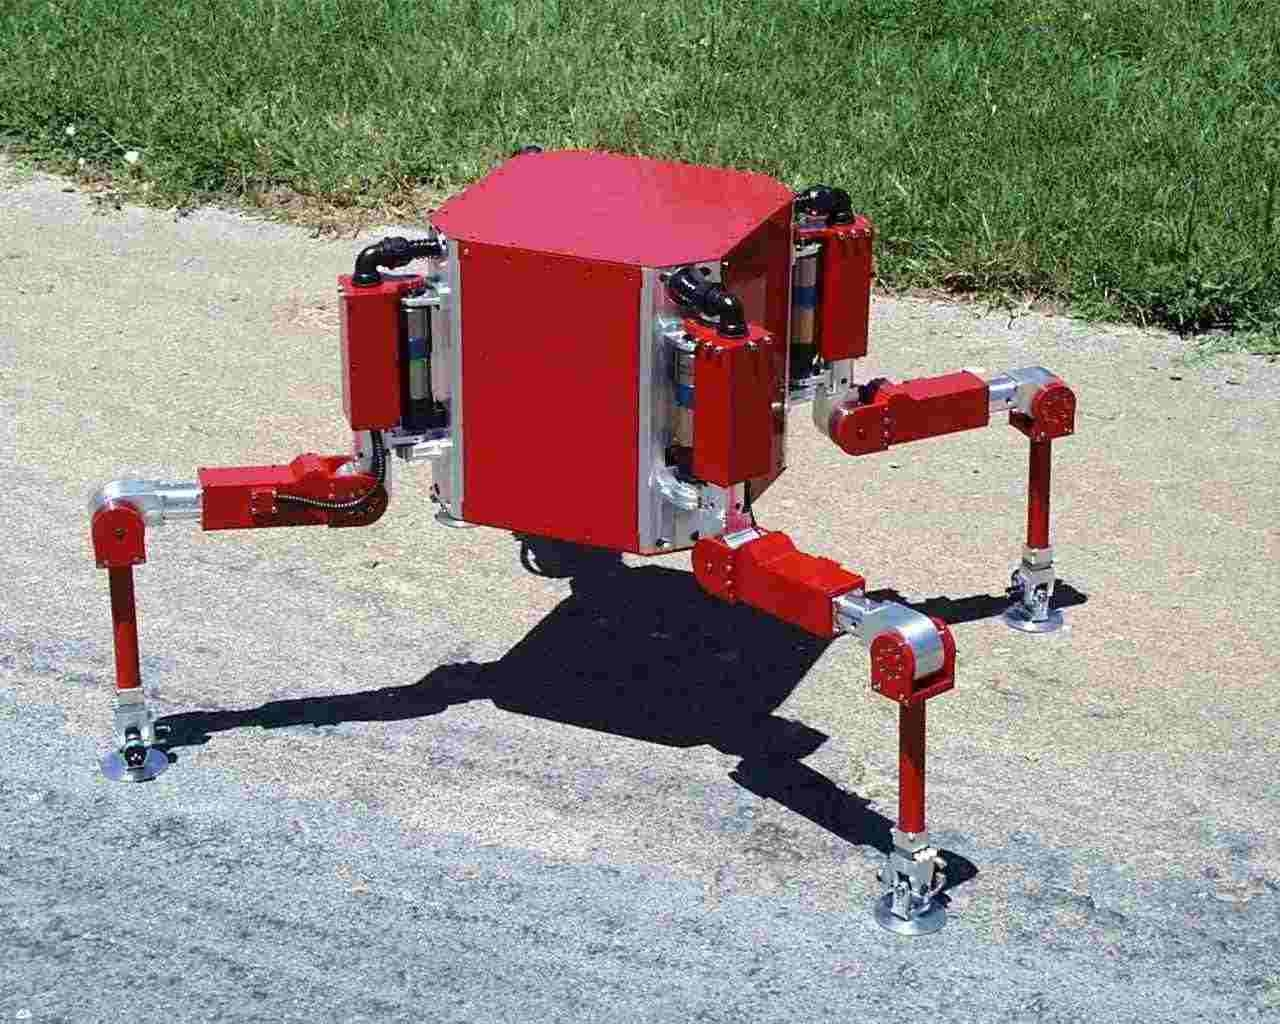
\includegraphics[width=80mm]{intro24}}
\end{minipage}
\hfill
\begin{minipage}{0.49\linewidth}
\center{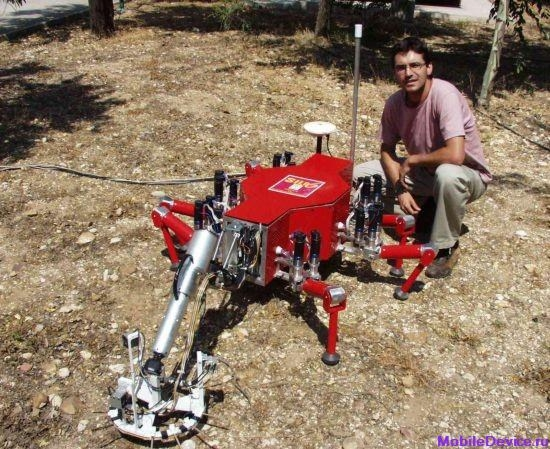
\includegraphics[width=80mm]{intro25}}
\end{minipage}
\caption{Silo 4 (четырехногий) и Silo 6 (шестиногий). Испания}
\label{fig21}
\end{figure}
 
\clearpage

Наконец, на рис.\ref{fig22} – хорошо известные современные разработки фирмы Boston Dynamics, США, роботы Big Dog и Alpha Dog.

\begin{figure}[here]
\begin{minipage}{0.49\linewidth}
\center{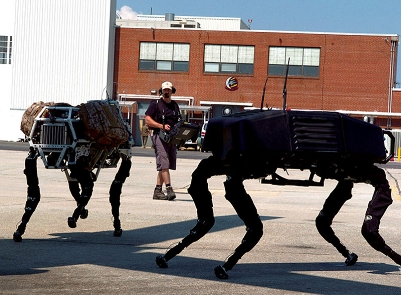
\includegraphics[width=80mm]{intro26}}
\end{minipage}
\hfill
\begin{minipage}{0.49\linewidth}
\center{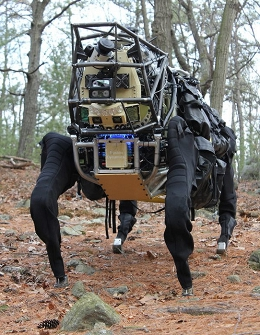
\includegraphics[width=80mm]{intro27}}
\end{minipage}
\caption{Роботы Big Dog (слева) и Alpha Dog}
\label{fig22}
\end{figure} 

%\clearpage

Сказанное о технологиях перехода к шагающим машинам как роботам с программным синтезом движения полностью подтверждается, например, работами по многоногим шагающим роботам в России в Волгоградском государственном техническом университете (ВолгГТУ). Здесь создаются машины с так называемыми цикловыми механизмами ходьбы и машины с оригинальными ортогональными приводами движителей. Образцом таких разработок может служить шагающая машина "Восьминог", показанная на рис.\ref{fig23}. В этой разработке механизмы шагания также построены на идее лямбда-механизма Чебышева, поэтому цикл шагания фактически создается механическим устройством ноги. Возможно, это несколько ограничивает адаптационные возможности машины, но ее бесспорным преимуществом является значительная простота системы управления и весьма высокая опорная проходимость машины. Машина способна двигаться и работать на очень слабых грунтах (рис. ~\ref{fig23}).

\begin{figure}[h]
\begin{minipage}{0.49\linewidth}
\center{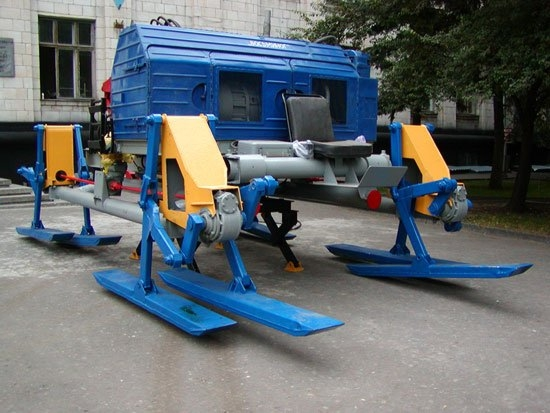
\includegraphics[width=80mm]{intro28}}
\end{minipage}
\hfill
\begin{minipage}{0.49\linewidth}
\center{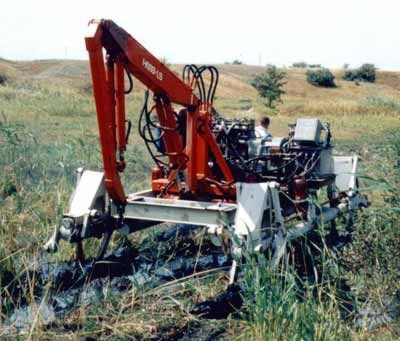
\includegraphics[width=80mm]{intro29}}
\end{minipage}
\caption{Машина "Восьминог" ВолгГТУ. Волгоград}
\label{fig23}
\end{figure} 

Однако, в дальнейшем авторы предприняли еще одно направление работ – создание машин с ортогональными шагающими движителями. На рис.\ref{fig24} показан средний макет восьминогого робота с ортогональными приводами (характерный размер машины – 1 м). Движитель организован как два модуля с четырьмя опорами каждый и для реализации поворота машины модули могут поворачиваться друг относительно друга. Наличие в аппарате большого числа степеней свободы приводит к необходимости бортового компьютерного управления этой машиной. Система управления для этой машины разрабатывается в ИПМ им. М.В.Келдыша РАН.

\begin{figure}[here]
\center{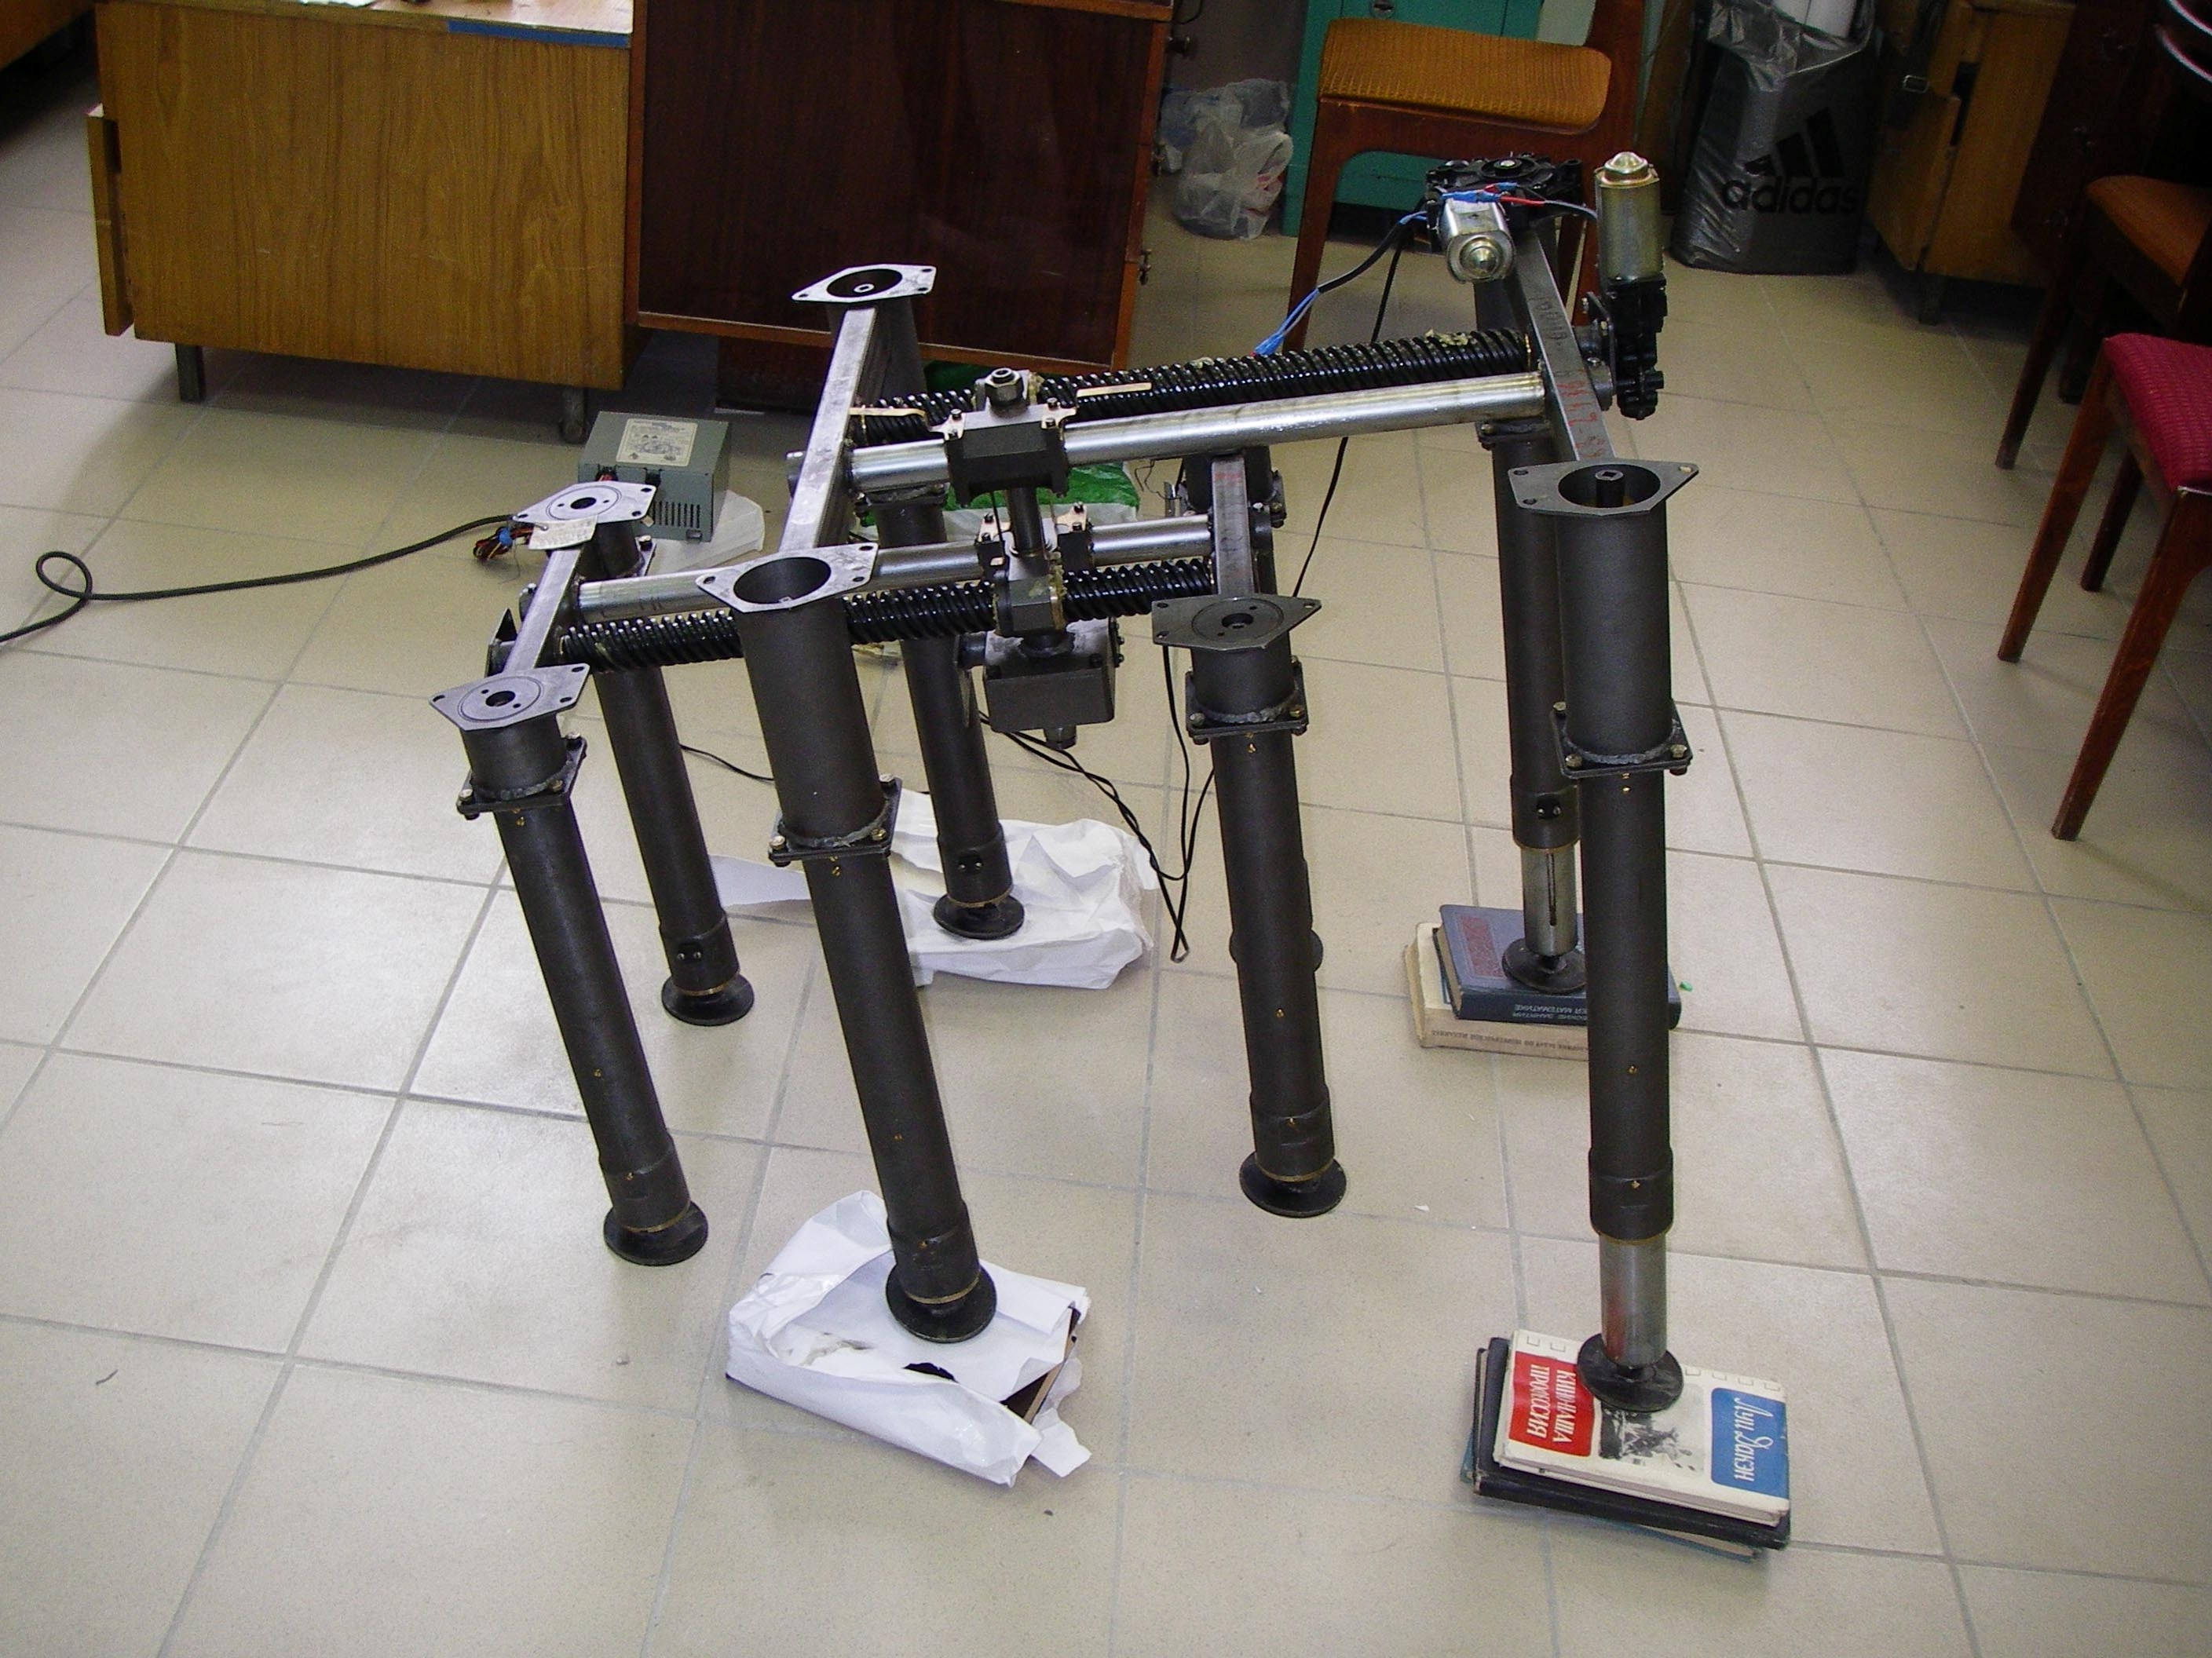
\includegraphics[width=90mm]{intro30}}
\caption{Робот с ортогонально-поворотным движителем. ВолгГТУ. Волгоград}
\label{fig24}
\end{figure}
\begin{figure}[here]
\center{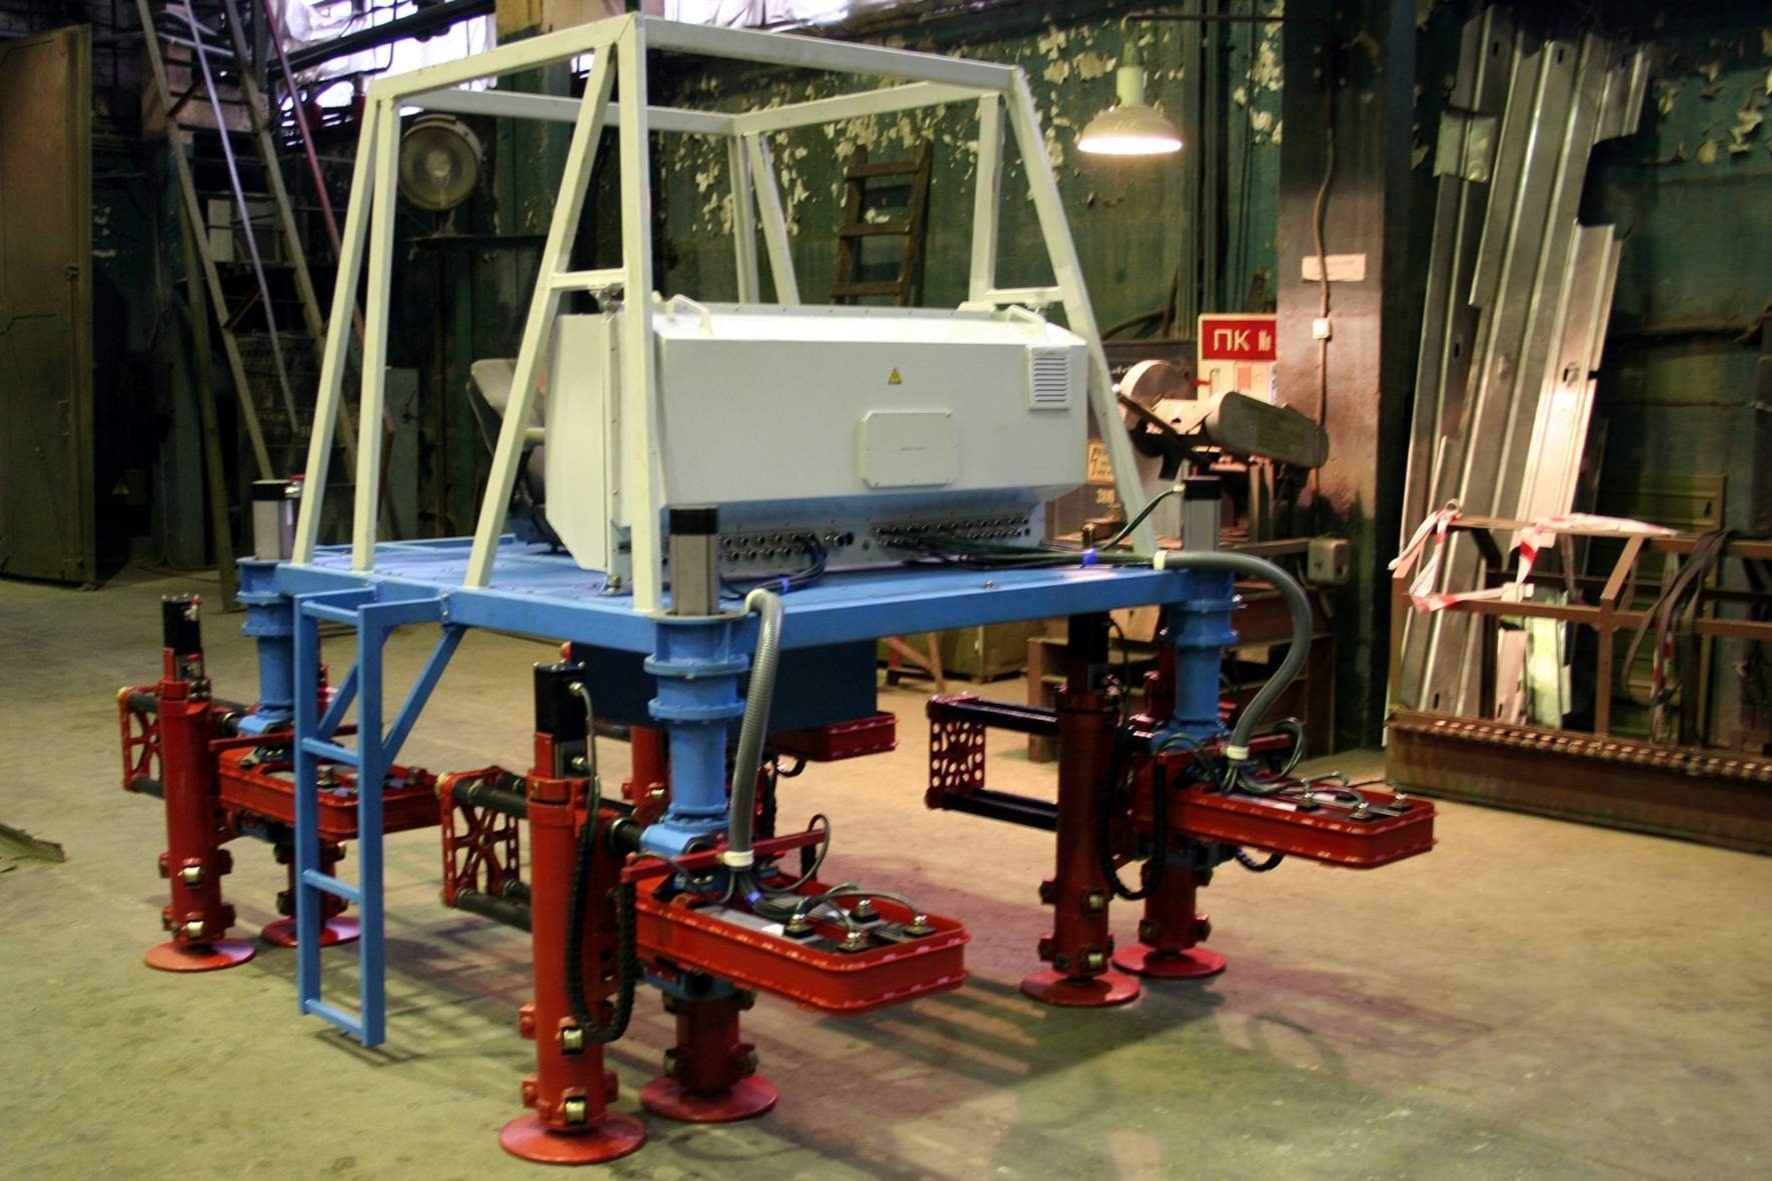
\includegraphics[width=90mm]{intro31}}
\caption{Шагающая машина "Ортоног". Волгоград}
\label{fig25}
\end{figure} 

Как развитие этих исследований в ВолГТУ выполняется проект по созданию большой шагающей машины с 4-мя спаренными ортогонально-поворотными движителями, общим весом 2 т и грузоподъемностью до 1 т (рис.\ref{fig25}). В настоящее время завершено изготовление машины, начаты интенсивные работы по программированию ее системы управления. Укажем некоторые важные проекты мини-гексаподов. Они приведены на рис.\ref{fig26} и рис.\ref{fig27}.

\begin{figure}[here]
\begin{minipage}{0.49\linewidth}
\center{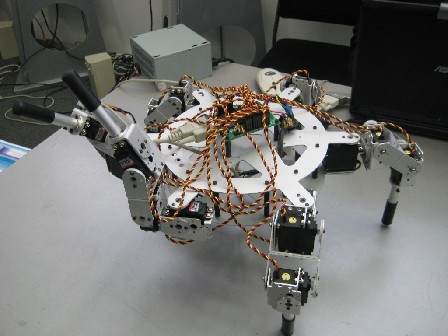
\includegraphics[width=70mm]{intro38}}
\end{minipage}
\hfill
\begin{minipage}{0.49\linewidth}
\center{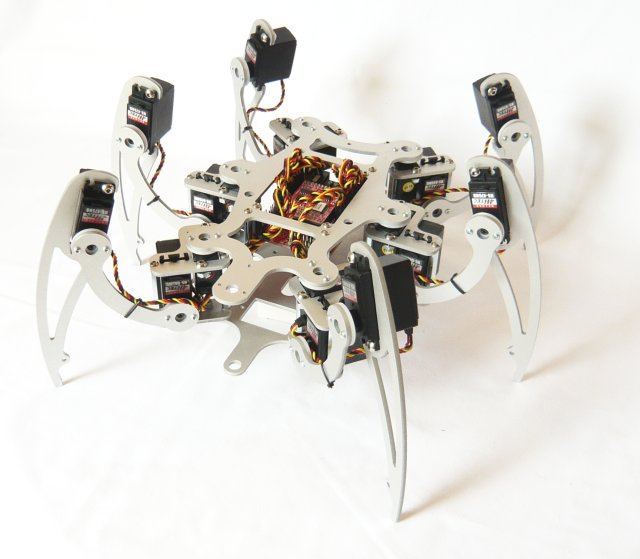
\includegraphics[width=70mm]{intro39}}
\end{minipage}
\caption{Lynxmotion (слева) и MSR-H01-01(справа)}
\label{fig26}
\end{figure} 

\begin{figure}[here]
\begin{minipage}{0.49\linewidth}
\center{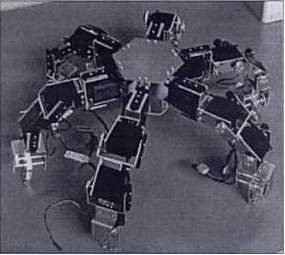
\includegraphics[width=70mm]{intro40}}
\end{minipage}
\hfill
\begin{minipage}{0.49\linewidth}
\center{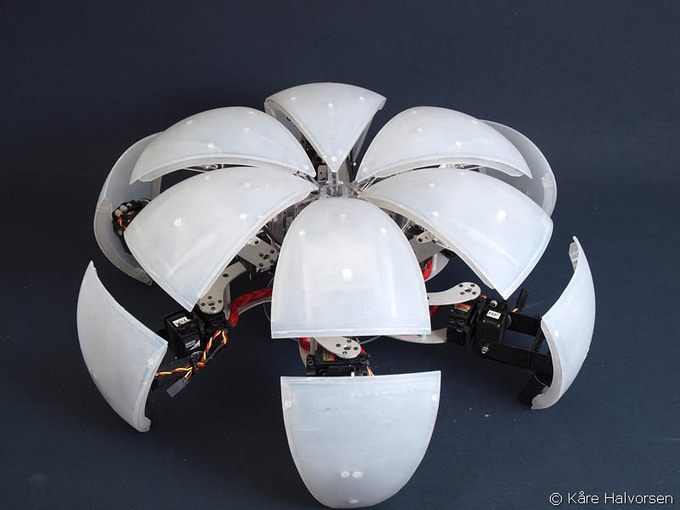
\includegraphics[width=70mm]{intro41}}
\end{minipage}
\caption{ARTEX (слева) и MORPHEX (справа)}
\label{fig27}
\end{figure}

Нетрудно заметить, что все это небольшие машины (размер в поперечнике меньше 0.5 м), достаточно легкие, предназначенные главным образом для исследований проблем шагающего движения. На проект робота MORPHEX (рис. ~\ref{fig27}) следует обратить особое внимание - это робот-трансформер, который способен принимать шарообразную форму и катиться по поверхности. При необходимости он снова раскрывается в шестиногий аппарат.

Анализируя приведенные обзорные данные, отметим с одной стороны удивительную кинематическую схожесть различных проектов, выполненных в разных лабораториях. Можно считать, что сформировались несколько типовых классов шагающих машин – основные из них, это малые, до 0.5 м, средние, порядка 1 м, и большие роботы.


\newpage
\subsection*{Этапы создания шагающей машины}
Одним из первых этапов в проектировании шагающего робота является выбор конструкции и кинематики ноги и определение числа ног машины. Оптимальное количество ног (и их конструкция) определяются назначением шагающей машины (ШМ) и средой ее применения. 
Число ног, равное шести, является оптимальным с точки зрения наибольшей свободы и скорости передвижения в рамках статической устойчивости. 

\emph{Четырехногая} ШМ обычно имеет меньшие габариты, вес и более простую конструкцию, она также может двигаться в рамках статической устойчивости. Но ее профильная и опорная проходимость меньше, чем у шестиногой, скорость движения также меньше при прочих равных условиях.

\emph{Двуногая} машина может иметь самые малые размеры, но ее движение возможно только в рамках динамической устойчивости, организация такого движения весьма сложна. 

\emph{Многоногие} машины имеют большую грузоподъемность при заданных ограничениях давления на грунт и размер стоп. 
Говоря о кинематике ноги, укажем основные биологические прототипы. Они показаны на рис. \ref{fig28}. Среди всего разнообразия в живой природе наибольший интерес как основные прототипы представляют конечности насекомых и рептилий (первый рисунок на рис.\ref{fig28}), млекопитающих (средний рисунок), птиц (правый рисунок).


%\begin{figure}[here]
%\begin{minipage}{0.40\linewidth}
%\center{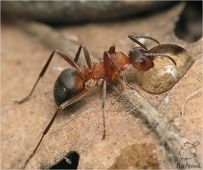
\includegraphics[width=30mm]{intro32}}
%\end{minipage}
%\hfill
%\begin{minipage}{0.40\linewidth}
%\center{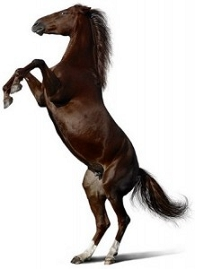
\includegraphics[width=30mm]{intro33}}
%\end{minipage}
%\hfill
%\begin{minipage}{0.40\linewidth}
%\center{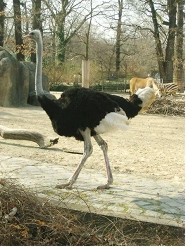
\includegraphics[width=30mm]{intro34}}
%\end{minipage}
%\caption{Ноги биологических существ-прототипов}
%\label{fig26}
%\end{figure}


\begin{figure}[here]
\center{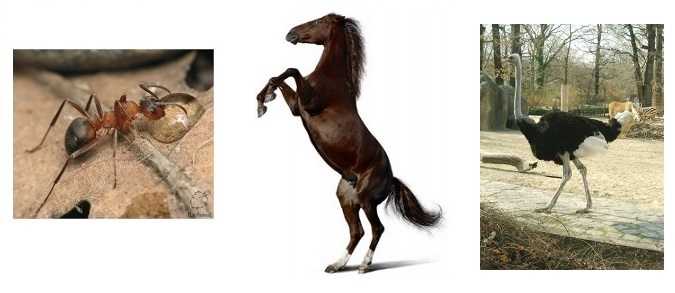
\includegraphics[width=150mm]{intro32-34}}
\caption{Ноги биологических существ-прототипов}
\label{fig28}
\end{figure}

История и примеры развития шагающих машин таковы, что наибольший интерес у разработчиков вызывала и вызывает первая схема – так называемые инсектоморфные (насекомоподобные) ноги. Этот вариант реализовывался в подавляющем большинстве конструкций. На рис.\ref{fig29} показана типичная схема и конструкция такой ноги с 5-ю степенями подвижности.
После выбора схемы шагающего движителя возникают общие вопросы выбора компоновки, системы управления, сенсоров, программного обеспечения робота.
\begin{figure}[here]
\begin{minipage}{0.49\linewidth}
\center{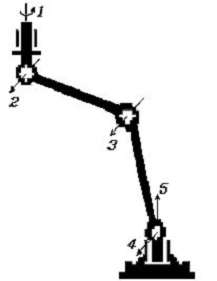
\includegraphics[width=50mm]{intro35}}
\end{minipage}
\hfill
\begin{minipage}{0.49\linewidth}
\center{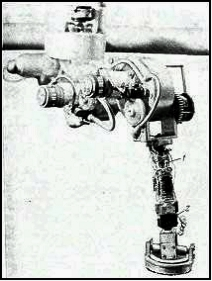
\includegraphics[width=50mm]{intro36}}
\end{minipage}
\caption{Инсектоморфная конечность}
\label{fig29}
\end{figure}

\begin{figure}[here]
\center{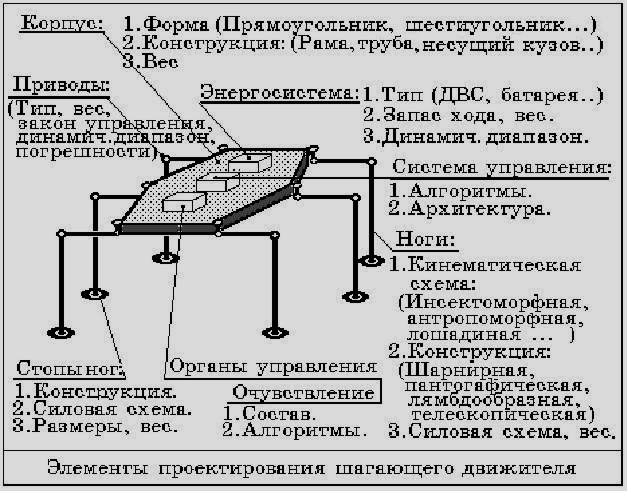
\includegraphics[width=110mm]{intro37}}
\caption{Этапы проекта шагающей машины}
\label{fig30}
\end{figure} 

Соответствующая общая схема этапов проектирования ШМ приведена на рис.\ref{fig30}.

В заключение этого обзора, подведем итог. Шагающий способ представляет основной интерес для движения по заранее неподготовленной местности с препятствиями. Традиционные колесные и гусеничные транспортные машины оставляют за собой непрерывную колею, а в случае передвижения шагами, взаимодействие с грунтом происходит только в местах опоры стопы. При шагающем способе меньше разрушается грунт, что, например, важно в тундре. Помимо этого шагающий способ передвижения обладает и большей специфической проходимостью на пересеченной местности вплоть до возможности передвигаться прыжками и т.п. При движении по достаточно гладким и подготовленным поверхностям способ перемещения при помощи шагания уступает колесному в экономичности, скорости передвижения и простоте управления.
Отмечая проблемы, решение которых не завершено, укажем следующие. Одной из проблем, которой уделяется существенное внимание при проектировании мобильных шагающих аппаратов, является уменьшение необходимой мощности источников питания и сокращение затрат энергии. Необходимо повысить к.п.д. многоногих механизмов, т.е. уменьшить потребляемую мощность и повысить развиваемую мощность. В самом деле, если учесть, что в общем случае каждая из конечностей имеет две-три-четыре степени подвижности и управление каждой из степеней сопряжено с определенными затратами энергии, то очевидно, что сравнение шагающих и колесных транспортных средств по к.П.Д. будет не в пользу первых. В связи с этим важная цель, к достижению которой должны стремиться исследователи сегодня, заключается в создании экспериментальных шагающих аппаратов, способных на практике продемонстрировать сочетание высоких функциональных возможностей с достаточно большой развиваемой мощностью при сниженных затратах энергии. Возможно, это потребует создания новых приводов для ШМ.
Отдельное важнейшее направление – создание новых перспективных планетных роверов. Следует добавить, что, по всей вероятности, эти потребности будут удовлетворяться, прежде всего, за счет шагающих аппаратов с шестью конечностями.

\subsection*{Современное состояние}
Много кто способен сейчас сделать робота буквально на коленке. Управляющая электроника и необходимые двигатели стали доступней в последнее время. Обычный человек может получить доступ к самым современных технологиям производства, таким как лазерная резка или 3d печать деталей из пластика. Современные САПР (Система Автоматизированного Проектирования) комплексы позволяют получить прототип детали в считанные часы. Стоимость комплектующих постоянно уменьшается, а качество и мощность постоянно растут. Всё это понижает входной порог в современной робототехнике. В сети интернет публикуется большое количество работ от энтузиастов одиночек, которые увлекаются созданием различных устройств и роботов. Не нужно отдельное конструкторское бюро и заводские условия чтобы создавать роботов в наши дни. Достаточно заказать подходящую электронику по интернету и напечатать механику на 3d принтере или вырезать лазером из листового металла необходимые детали и робот готов. Не все детали можно напечатать на 3d принтере, некоторые придётся изготовить обычным методом, на токарном или фрезерном станке, но можно упростить себе задачу и заказывать через интернет.

Робототехника получает второе дыхание. Лет сорок назад людям казалось, что пройдёт всего каких-то лет 30-40 и будет создан искусственный интеллект и роботы будут повседневным атрибутом нашей жизни. Роботам можно будет поручить рутинную, опасную работу, а человеку останется много свободного времени. В чём-то прогнозы сбылись, современные автоматизированные производственные линии значительно повысили эффективность труда, там, где раньше работали десятки токарей, теперь достаточно поставить один обрабатывающий центр и он будет работать круглосуточно, без больничных и отпусков.

Все это не совсем робототехника, это просто сложные автоматы, созданные людьми. Станки принципиально не изменились, произошла замена электроники и двигателей. Всё так же далеко до создания искусственного интеллекта, как и 30-40 лет назад. Подавляющее большинство роботов годится только для лабораторного использования, по-настоящему способных работать в человеческой среде аппаратов очень мало. Не всё так плохо, тенденция к появлению автономных аппаратов способных работать в неподготовленных условиях определенно наблюдается. Значительного успеха в этой области достигла американская компания Boston Dynamics. Первый значительный успех произошёл в 2005 году, когда публике был представлен робот BigDog \cite{BigDog}. 

\begin{figure}[t]
\center{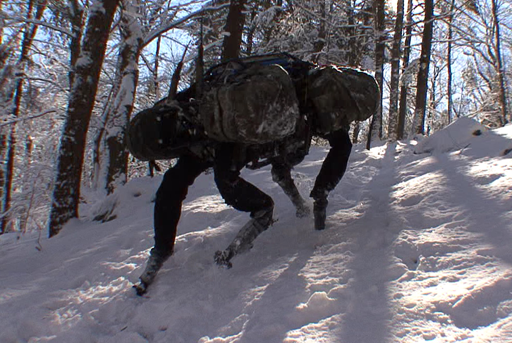
\includegraphics[width=100mm]{BigDog_Snow}}
\caption{BigDog}
\end{figure}

BigDog — четырёхногий робот с адаптивным управлением, созданный в 2005 году фирмой Boston Dynamics совместно с Foster-Miller, Лабораторией реактивного движения (NASA) и Harvard University Concord Field Station.

Проект BigDog финансируется агентством перспективных военных разработок (Defense Advanced Research Projects Agency, DARPA) с надеждой на то, что он сможет переносить снаряжение и помогать солдатам на территории, где не способен передвигаться обычный транспорт. Вместо колёс и гусениц BigDog использует четыре ноги. В ногах находится большое количество разнообразных сенсоров. Также у BigDog имеется лазерный гироскоп и система бинокулярного зрения.
Длина робота BigDog — 0,91 метр, высота 0,76 метра, вес 110 килограммов. В настоящее время он способен передвигаться по труднопроходимой местности со скоростью 6,4 км в час, перевозить 154 кг груза и подниматься на 35 градусную наклонную плоскость. Его передвижение контролирует компьютерная система, которая получает данные от различных сенсоров. Навигация и равновесие также управляются этой системой.
BigDog упоминается в статьях New Scientist, Popular Science, Popular Mechanics и Wall Street Journal, а также в нескольких видео на сайте Youtube.
18 марта 2008 года Boston Dynamics выпустила видео о новом поколении робота BigDog. Видео показывает возможность робота ходить по ледяной поверхности и возможность восстанавливать равновесие после удара сбоку.

BigDog приводится в движение двухтактным одноцилиндровым двигателем от карта со скоростью вращения 9000 об/мин, из-за чего слышен громкий звук мотора. В последующих версиях робота планируется исправить этот демаскирующий недостаток. Мотор служит приводом для гидронасоса, который в свою очередь питает гидравлику ног. В каждой из ног установлено по 4 гидравлических привода (два для бедренного сустава, и по одному для коленного и голеностопного суставов) общим числом 16. Каждый из гидравлических двигателей состоит из гидроцилиндра, сервоклапана, а также датчиков положения и усилия. Робот обладает хорошей устойчивостью: во время испытаний он не падал при проходе по льду и при сильных толчках.
Бортовой компьютер робота представляет собой упрочненный вариант платформы PC/104 с процессором класса Pentium под управлением ОС QNX.

В 2012 году была представлена новая версия аппарата, получившая название Legged Squad Suppor System(LS3)\cite{LS3}. Новая версия аппарата отличается большей грузоподъёмностью и возможностью работать в сложных условиях.
\begin{figure}
\center{\includegraphics[width=100mm]{DSC_0502}}
\caption{Legged Squad Support System - LS3}
\end{figure}

Аппарат способен нести до 180кг нагрузки, преодолевать пересеченную местность, быстро реагировать и работать в тихом, беззвучном режиме, когда это необходимо. Система стереозрения, установленная в передней части аппарата, позволяет распознавать ведущего и следовать за ним в автоматическом режиме. Добавлена опция восприятия голосовых команд. Доработаны алгоритмы ходьбы по сложной, каменистой местности, доработан переход на трусцу и бег на ровных поверхностях. Планируется поставить первые серийные системы LS3 в действующие отряды морской пехоты США к 2014 году.


Шестиногие аппараты относятся к классу статически устойчивых аппаратов. Шестиногие роботы могут передвигаться, сохраняя статическую устойчивость. Это следует из того, что для шестиногого аппарата существуют классы походок, для которых верно, что в каждый момент времени три ноги аппарата находятся в опорной фазе и проекция центра масс робота попадает во внутреннюю область опорного треугольника. Среди аппаратов подобного класса широко известно семейство аппаратов Lauron и шагающее шестиногое шасси Mantis компании Micromagic Systems.


\begin{figure}[h]
\begin{minipage}[h]{0.49\linewidth}
\center{\includegraphics[width=80mm]{800px-Lauron4c_2009_FZI_Karlsruhe}}
\caption{LAURON IV}
\end{minipage}
\begin{minipage}[h]{0.49\linewidth}
\center{\includegraphics[width=80mm]{8586212180_99ffd2e15e}}
\caption{Carausius morosus}
\end{minipage}
\end{figure}


LAURON --- шестиногий шагающий робот, который разрабатывается в Исследовательском Центре Информационных Технологий (FZI) в Карлсруэ, Германия. Робот являются имитацией реального насекомого Carausius Morosus из семейства палочных насекомых. Создание шагающего робота началось с фундаментального исследования в области шестиногой ходьбы в начале 1990-х годов и привело к созданию первых роботов, названных Lauron. В 1994 году первый робот был представлен публике на выставке CeBIT в Ганновере. Стоит отметить, что разработки  по шестиногим шагающим аппаратам велись в ИПМ имени М.В. Келдыша ещё в 70-80 годы.

Первое поколение Lauron, в отличие от более поздних версий, управлялось при помощи искусственной нейронной сети. Именно поэтому первый робот получил название LAURON. От немецкого - LAUfROboter Neuronal gesteuert (English: Walking Robot, Neural Controlled).

\begin{figure}
\center{\includegraphics[width=80mm]{LAURON_V_-_2013_FZI_Karlsruhe}}
\caption{LAURON V}
\end{figure}

Самая последняя версия семейства LAURON была представлена в 2013 году, на Международной Конференции по Робототехнике и Автоматизации (ICRA), в Карлсруэ, Германия. Кинематика робота была улучшена, путём добавления дополнительного вращательного шарнира в бедренный сустав каждой ноги \cite{Roennau2013}. Такая модификация позволит роботу всегда держать плоскость ноги в вертикальном положении, что снижает нагрузку на шарниры ног при движении по крутому склону насыпи. Так же, дополнительная степень свободы теперь позволяет аппарату выполнять различные манипуляции с объектами, используя пару передних ног как пару манипуляторов. 

Аналогичный проект шагающего шестиногого аппарата \cite{Langosz2013} ведёт Центр Инновационной Робототехники (Robotics Innovation Center) под эгидой Немецкого Исследовательского Центра Искусственного Интеллекта (DFKI GmbH), город Бремен, Германия. 

\begin{figure}[h]
\center{\includegraphics[width=100mm]{20110225_SpaceClimber_Cebit_Foerderer}}
\caption{Space Climber}
\end{figure}

Цель программы SpaceClimber состоит в разработке аппарата с инсектоморфной (насекомоподобной) кинематикой \cite{1984}, способного энергетически эффективно преодолевать крутые склоны. Предполагается, что аппарат будет автономно исследовать внеземные кратеры, например, на Луне или Марсе. Аппарат будет доставляться в зону исследования на планетоходе и выгружаться при помощи специального крана-манипулятора установленного на ровере. Планетоход так же разрабатывается в Центре Инновационной Робототехники. Проект находится на стадии испытаний, на специальном лунном полигоне, имитирующем склоны лунных кратеров. По итогам программы планируется получить подтверждение, что шагающие аппараты являются основным инструментом в вопросе исследований труднопроходимых поверхностей, кратеров, расщелин и т.д.

 Компания Micromagic Systems основана в 1999 году и занимается разработкой аниматронов - роботов для создания анимированных персонажей и спецэффектов в кино. Так же, компания занимается разработкой управляющих систем для различных робототехнических систем, занимается производством механизированных кукол для кукольных шоу. В 2001 году компанией был представлен робот на модельных сервомашинах -  hexapod V1. Стоит отметить, что это был один из первых шагающих роботов собранных на сервомашинках. Робот hexapod v1 был способен передвигаться по ровной поверхности различными походками.

Шагающее транспортное средство Mantis Hexapod было представлено компанией Micromagic Systems в 2012 году.

\begin{figure}
\center{\includegraphics[width=100mm]{1209116_628585443829653_1753427504_n}}
\caption{Шагающий аппарат Mantis}
\end{figure}

Mantis весит 1900 кг, диаметр аппарата составляет 5 метров. Аппарат оборудован турбодизельным двигателем Perkins 2.2 мощностью 42 кВт и сопряженным гидравлическим насосом на 165 атмосфер. Шарниры приводятся в движения при помощи гидроцилиндров через пропорциональные клапаны управления. Аппарат оборудован бортовым компьютером на базе платформы PC/104 под управлением операционной системы Linux и различными системами датчиков, таких как, датчики давления в цилиндрах, датчики положения в шарнирах, силовые контактные датчики в стопах, датчик угла наклона корпуса. Так же, используется другая вспомогательная электроника для компьютерного управления двигателем, сбора информации с датчиков и её последующей передачи по CAN шине в бортовой компьютер.


В итоге по данным приведенного обзора сделаем следующий вывод. Рассмотренные данные показывают, что подавляющее количество конструкций - это шестиногие роботы с инсектоморфной кинематикой ног. Поэтому далее в настоящей работе будут рассматриваться инсектоморфные ноги. В дополнение рассмотрим аппарат с ортогональными движителями.


%%%%%%%%%%%%
\clearpage
Обзор, введение в тему, обозначение места данной работы в мировых исследованиях и т.п.

\textbf{Целью} данной работы является \ldots

Для~достижения поставленной цели необходимо было решить следующие задачи:
\begin{enumerate}
  \item Исследовать, разработать, вычислить и т.д. и т.п.
  \item Исследовать, разработать, вычислить и т.д. и т.п.
  \item Исследовать, разработать, вычислить и т.д. и т.п.
  \item Исследовать, разработать, вычислить и т.д. и т.п.
\end{enumerate}

\textbf{Основные положения, выносимые на~защиту:}
\begin{enumerate}
  \item Первое положение
  \item Второе положение
  \item Третье положение
  \item Четвертое положение
\end{enumerate}

\textbf{Научная новизна:}
\begin{enumerate}
  \item Впервые \ldots
  \item Впервые \ldots
  \item Было выполнено оригинальное исследование \ldots
\end{enumerate}

\textbf{Научная и практическая значимость} \ldots

\textbf{Степень достоверности} полученных результатов обеспечивается \ldots Результаты находятся в соответствии с результатами, полученными другими авторами.

\textbf{Апробация работы.}
Основные результаты работы докладывались~на:
перечисление основных конференций, симпозиумов и т.п.

\textbf{Личный вклад.} Автор принимал активное участие \ldots

\textbf{Публикации.} Основные результаты по теме диссертации изложены в ХХ печатных изданиях~\cite{bib1,bib2,bib3,bib4,bib5},
Х из которых изданы в журналах, рекомендованных ВАК~\cite{bib1,bib2,bib3}, 
ХХ --- в тезисах докладов~\cite{bib4,bib5}.

\textbf{Объем и структура работы.} Диссертация состоит из~введения, четырех глав, заключения и~двух приложений. Полный объем диссертации составляет ХХХ~страница с~ХХ~рисунками и~ХХ~таблицами. Список литературы содержит ХХХ~наименований.

\clearpage    % Введение
\chapter{История}							% Заголовок
\addcontentsline{toc}{chapter}{История}	% Добавляем его в оглавление

История создания шагающих механизмов очень богата и уходит в глубокую древность. Одно из первых упоминаний в литературных источниках (Reconstruction designs of lost ancient Chinese machinery" By Hong-Sen Yan ,http://cyberneticzoo.com/walking-machines/480-bc-wooden-horse-carriage-lu-ban/) датируется 480 годом до нашей эры - деревянная лошадь с повозкой, автор --- Лю Бан, Китай. Современную репродукцию лошади с повозкой можно видеть на рис. \ref{img:wooden_horse}.

\begin{figure}[ht]
	\begin{minipage}[ht]{0.49\linewidth}
		\centering{\includegraphics[width=0.8\linewidth]{Introduction/intro1} \\ а)}
	\end{minipage}
	\hfill
	\begin{minipage}[ht]{0.49\linewidth}
		\centering{\includegraphics[width=0.8\linewidth]{Introduction/intro2} \\ б)}
	\end{minipage}
	\caption{Деревянная лошадь с повозкой, 480 год до н.э. Лю Бан, Китай}
	\label{img:wooden_horse}  
\end{figure}

Одним из первых ученых нового времени, заинтересовавшихся задачей математического анализа перемещения стопоходящих животных, стал известный русский математик и механик П.Л. Чебышев. В 1878 г. на Всемирной выставке в Париже была продемонстрирована так называемая стопоходящая машина, имитирующая движение четырехногого животного при ходьбе. Кинематическая схема машины состоит из четырех лямбда-механизмов Чебышева. В настоящее время действующая реплика машины хранится в московском Политехническом музее. Модель стопоходящей машины изображена на рис. \ref{img:chebishev}

\begin{figure}[ht]
	\centering
	\includegraphics[width = 0.5\linewidth]{Introduction/intro3}
	\caption{Стопоходящая машина П.Л. Чебышева. 1878 г}
	\label{img:chebishev}
\end{figure}

П.Л. Чебышев является одним из основоположников математической теории синтеза механизмов.

В СССР исследования по тематике шагающих роботов начинались в ИМАШ АН СССР в ИПМ АН СССР (позднее ИПМ им.М.В.Келдыша РАН). В ИПМ АН СССР работы велись под руководством Д.Е. Охоцимского. В периода 1972-1975гг были созданы первые макеты многоногих шагающих машин. На рис. \ref{img:imash_ran}

\begin{figure}[ht]
	\centering
	\includegraphics[width = 0.5\linewidth]{Introduction/intro4}
	\caption{Шагающая машина ИМАШ РАН}
	\label{img:imash_ran}
\end{figure}

В шагающем аппарате ИМАШ РАН использована оригинальная кинематика ног --- ортогональная. Каждая из шести ног состоит из пары штоковых механизмов, соединенных между собой под прямым углом. Один из штоков жестко крепится к корпусу, второй шток используется для удержания веса аппарата. Преимущество данной ортогональной кинематики ноги состоит в простом синтезе движения.

На рис. \ref{img:IPM_robots} изображены макеты шестиногих шагающих аппаратов, созданных в Институте Прикладной Математики АН СССР.

\begin{figure}[ht]
	\begin{minipage}[ht]{0.49\linewidth}
		\centering{\includegraphics[width=0.5\linewidth]{Introduction/intro5} \\ а)}
	\end{minipage}
	\hfill
	\begin{minipage}[ht]{0.49\linewidth}
		\centering{\includegraphics[width=0.5\linewidth]{Introduction/intro6} \\ б)}
	\end{minipage}
	\caption{Шагающие роботы ИПМ АН СССР. Фото 1975г}
	\label{img:IPM_robots}  
\end{figure}

Аппараты оснащены инсектоморфными (насекомоподобными, от англ. insect --- насекомое) ногами. Каждая нога обладает тремя степенями подвижности. На рисунке \ref{img:IPM_robots} аппараты оснащены лазерным измерителем расстояний --- ЛИР. С помощью ЛИР система управления робота получала информацию об окружающем пространстве и принимала решение о параметрах движения. Наличие шести ног позволяет аппарату передвигаться статически устойчивой походкой. Именно наличие множества классов статически устойчивых походок определило интерес к многоногим машинам.

В результате совместных работ ИПМ им М.В. Келдыша АН СССР и ВНИИТРАНСМАШ в 1975г создан макет шестиногой шагающей машины НМША (Натурный Макет Шагающего Аппарата) способной нести на себе человека оператора-водителя. Масса машины составляет 750кг, скорость движения 0,7 км/ч, грузоподъемность 50кг, дорожный просвет 1,5 м. Аппарат НМША изображен на рис. \ref{img:NMSHA}

\begin{figure}[ht]
	\begin{minipage}[ht]{0.49\linewidth}
		\centering{\includegraphics[width=0.8\linewidth]{Introduction/intro7} \\ а)}
	\end{minipage}
	\hfill
	\begin{minipage}[ht]{0.49\linewidth}
		\centering{\includegraphics[width=0.8\linewidth]{Introduction/intro8} \\ б)}
	\end{minipage}
	\caption{Аппарат НМША. 1975г}
	\label{img:NMSHA}  
\end{figure}

Обозначенные исследования на базе ИПМ им.М.В.Кледыша продолжаются в настоящее время. На рис. \ref{img:IPM_now} показан макет робота третьего поколения. На роботе установлены современные электродвигатели, бортовая процессорная система управления. На аппарате установлен необходимый набор сенсоров и датчиков.

\begin{figure}[ht]
	\begin{minipage}[ht]{0.49\linewidth}
		\centering{\includegraphics[width=0.8\linewidth]{Introduction/intro9} \\ а)}
	\end{minipage}
	\hfill
	\begin{minipage}[ht]{0.49\linewidth}
		\centering{\includegraphics[width=0.8\linewidth]{Introduction/intro10} \\ б)}
	\end{minipage}
	\caption{Шагающий робот ИПМ им.М.В.Келдыша РАН. Фото 2009 г}
	\label{img:IPM_now}  
\end{figure}

Работы по исследованию шагающих аппаратов ведутся в Институте Механики МГУ. На рис. \ref{img:masha} изображен макет шагающего робота МАША --- МАшина ШАгающая.

\begin{figure}[ht]
	\begin{minipage}[ht]{0.49\linewidth}
		\centering{\includegraphics[width=0.8\linewidth]{Introduction/intro11} \\ а)}
	\end{minipage}
	\hfill
	\begin{minipage}[ht]{0.49\linewidth}
		\centering{\includegraphics[width=0.8\linewidth]{Introduction/intro12} \\ б)}
	\end{minipage}
	\caption{МАША. Институт Механики МГУ.}
	\label{img:masha}  
\end{figure}

Проекты шагающих машин выполнены практически во всех технологически развитых странах. Приведем примеры иностранных разработок.

Одним из первых шагающих аппаратов в США является так называемая Калифорнийская лошадь --- Phoney Poney. Фотография макета изображена на рис. \ref{img:phoney_poney}

\begin{figure}[ht]
	\centering
	\includegraphics[width = 0.4\linewidth]{Introduction/intro13}
	\caption{Калифорнийская лошадь --- Phoney Pony. Университет Южной Калифорнии, 1968 г }
	\label{img:phoney_poney}
\end{figure}

Аппарат разработан и собран аспирантом Andrew Frank, под руководством профессора Robert McGhee в Университете Южной Калифорнии в 1968 году. Аппарат мог передвигаться рысью, галопом и другими походками четвероногих. Для управления робота использовалась ЭВМ размером с комнату, а управление осуществлялось по отдельному кабелю. Калифорнийская лошадь является первым примером практического применения теории конечных автоматов для управления движением шагающего аппарата.

На рис. \ref{img:walking_truck} изображена машина компании General Electric (США) ---  Walking Truck (Шагающий грузовик). Управление аппарата построено на копирующих манипуляторах. Оператор-водитель при помощи рук и ног передает движение через копирующие механизмы на соответствующие конечности аппарата.

\begin{figure}[ht]
	\centering
	\includegraphics[width = 0.5\linewidth]{Introduction/intro14}
	\caption{General Electrick Walking Truck, США, 1969 г}
	\label{img:walking_truck}
\end{figure}

Шагающий грузовик разрабатывался для нужд Министерства Обороны США. Предполагалось использовать Шагающий грузовик в труднопроходимых местах для перевозки военного оборудования, аммуниции, людей. Система управления аппарата оказалась слишком сложной для человека --- требовала от оператора-водителя огромного напряжения внимания и сил. Стало очевидным, что часть низкоуровневых функций управления, таких как координация движений ног аппарата и поддержание устойчивого положения аппарата, нужно перекладывать с человека на автоматику.

На следующих фотографиях изображены разработки второй половины ХХ века.

\begin{figure}[ht]
	\centering
	\includegraphics[width = 0.5\linewidth]{Introduction/intro15}
	\caption{Шетсиногий шагающий аппарат. Университет Огайо, профессор Robert McGhee. США}
	\label{img:intro15}
\end{figure}

\begin{figure}[ht]
	\begin{minipage}[ht]{0.49\linewidth}
		\centering{\includegraphics[width=0.8\linewidth]{Introduction/intro16} \\ а)}
	\end{minipage}
	\hfill
	\begin{minipage}[ht]{0.49\linewidth}
		\centering{\includegraphics[width=0.8\linewidth]{Introduction/intro17} \\ б)}
	\end{minipage}
	\caption{ASV - Adaptive Suspension Vehicle. Университет Огайо, Стенфордский Университет, США, 1984-1991гг}
	\label{img:ASV}  
\end{figure}

На рис. \ref{img:Plustech} показан аппарат разработки Финской компании Plustech Oy Ltd. Машина сконструирована для работы на лесоразработках в труднопроходимой местности. Основным преимуществом машины является высокая проходимость и сохранение верхнего плодородного слоя почвы при передвижении аппарата.

\begin{figure}[ht]
	\centering
	\includegraphics[width = 0.5\linewidth]{Introduction/intro18}
	\caption{Plustech Oy Ltd. Финляндия, 1999 г}
	\label{img:Plustech}
\end{figure}

На рисунках \ref{img:titan}---\ref{img:titan2} представлены японские разработки --- роботы семейства Titan.

\begin{figure}[ht]
	\begin{minipage}[ht]{0.49\linewidth}
		\centering{\includegraphics[width=0.8\linewidth]{Introduction/intro19} \\ а)}
	\end{minipage}
	\hfill
	\begin{minipage}[ht]{0.49\linewidth}
		\centering{\includegraphics[width=0.8\linewidth]{Introduction/intro20} \\ б)}
	\end{minipage}
	\caption{Titan 8, Япония, Лаборатория профессора Хиросе}
	\label{img:titan}  
\end{figure}

\begin{figure}[ht]
	\centering
	\includegraphics[width = 0.5\linewidth]{Introduction/intro21}
	\caption{Titan 11, Япония, Лаборатория профессора Хиросе}
	\label{img:titan2}
\end{figure}

На рис. \ref{img:lauron}---\ref{img:silo} представлены разработки Германии и Испании --- роботы семейств Lauron и Silo соответственно.

\begin{figure}[ht]
	\begin{minipage}[ht]{0.49\linewidth}
		\centering{\includegraphics[width=0.8\linewidth]{Introduction/intro22} \\ а)}
	\end{minipage}
	\hfill
	\begin{minipage}[ht]{0.49\linewidth}
		\centering{\includegraphics[width=0.8\linewidth]{Introduction/intro23} \\ б)}
	\end{minipage}
	\caption{Lauron 3, Lauron 4. Германия}
	\label{img:lauron}
\end{figure}

\begin{figure}[ht]
	\begin{minipage}[ht]{0.49\linewidth}
		\centering{\includegraphics[width=0.8\linewidth]{Introduction/intro24} \\ а)}
	\end{minipage}
	\hfill
	\begin{minipage}[ht]{0.49\linewidth}
		\centering{\includegraphics[width=0.8\linewidth]{Introduction/intro25} \\ б)}
	\end{minipage}
	\caption{Silo 4, Silo 6. Испания}
	\label{img:silo}
\end{figure}


На рис. \ref{img:bigdog} изображены самые современные аппараты --- хорошо известные Big Dog и Alpha Dog.

\begin{figure}[ht]
	\begin{minipage}[ht]{0.49\linewidth}
		\centering{\includegraphics[width=0.8\linewidth]{Introduction/intro26} \\ а)}
	\end{minipage}
	\hfill
	\begin{minipage}[ht]{0.49\linewidth}
		\centering{\includegraphics[width=0.8\linewidth]{Introduction/intro27} \\ б)}
	\end{minipage}
	\caption{Big Dog, Alpha Dog. США}
	\label{img:bigdog}
\end{figure}

На базе Волгоградского Государственного Технического Университета (ВолГТУ) создаются многоногие шагающие машины с ортогональной кинематикой ног и аппараты с циклическими механизмами ходьбы на основе механизмов схожих с лямбда-механизмами П.Л. Чебышева. На рис. \ref{img:octonog} изображена шагающая машина Восьминог. В кинематике аппарата параметры шагового цикла движения ноги-понтона определяются исключительно конструкцией ноги. 

\begin{figure}[ht]
	\begin{minipage}[ht]{0.49\linewidth}
		\centering{\includegraphics[width=0.8\linewidth]{Introduction/intro28} \\ а)}
	\end{minipage}
	\hfill
	\begin{minipage}[ht]{0.49\linewidth}
		\centering{\includegraphics[width=0.8\linewidth]{Introduction/intro29} \\ б)}
	\end{minipage}
	\caption{Восьминог, ВолГТУ, Волгоград}
	\label{img:octonog}
\end{figure}

Малое количество подвижностей в в ногах аппарата ограничивает адаптационные возможности. С другой стороны, система управления аппаратом сильно упрощается. Машина Восьминог с ногами-понтонами способна передвигаться по очень слабым грунтам (рис. \ref{img:octonog}).

На рис. \ref{img:ortho} изображен макет аппарата с оригинальной кинематикой. Аппарат состоит из двух четырехногих модулей. Каждая нога аппарата выдвигается и убирается при помощи отдельного электродвигателя и штокового механизма. Четырехногие модули аппарата связаны между собой при помощи специального шарнира с одной вращательной степенью подвижности и одной поступательной степенью подвижности. Четырехногие модули по очереди находятся в опорной фазе. Пока один модуль находится в опоре, второй переносится в опорную область при помощи межмодульного шарнира. Систему управления для данного макета разрабатывалась в ИПМ им.М.В.Келдыша РАН.

\begin{figure}[ht]
	\centering
	\includegraphics[width = 0.5\linewidth]{Introduction/intro30}
	\caption{Восьминогая шагающая машина с двухзвенным корпусом. ВолГТУ, Волгоград}
	\label{img:ortho}
\end{figure}

На базе ВолГТУ выполняется проект по созданию большой восьминогой шагающей машины. На рис. \ref{img:ortho2} изображен действующий макет аппарата.

\begin{figure}[ht]
	\centering
	\includegraphics[width = 0.5\linewidth]{Introduction/intro31}
	\caption{Шагающая машина Ортоног, Волгоград}
	\label{img:ortho2}
\end{figure}

Машина состоит из корпуса и четырех пар ног с ортогональной кинематикой. Каждая пара ног связана между собой общей базой к которой крепятся горизонтальные штоки. Общая база пары ног соединена через поворотный механизм с корпусом аппарата.    % История вопроса
%\chapter*{Глава 1. Многоногий шагающий аппарат c ортогональными движителями}
\addcontentsline{toc}{section}{Глава 1. Многоногий шагающий аппарат c ортогональными движителями}
В работе исследована кинематика многоногого шагающего аппарата с ортогональными движителями. Новизна такой кинематики состоит в уходе от использования природных кинематических схем ног, таких как нога насекомого или млекопитающего. Каждая нога обладает двумя поступательными взаимно перпендикулярными степенями свободы. В природе больше распространены вращательные соединения.

\begin{figure}[h]
\center{\includegraphics[width=100mm]{ortho_kinematics}}
\caption{Кинематическая схема аппарата}
\end{figure}

\section{Кинематическая схема аппарата}
Робот состоит из прямоугольного корпуса и четырех поворотных модулей. Поворотные модули будем называть H-модулями из-за сходства с русской буквой Н или латинской буквой H. Длина прямоугольного корпуса равна $2a$, ширина корпуса равна $2b$. Аппарат может перемещаться своим корпусом в горизонтальной плоскости $Oxy$. Положение корпуса задается координатами его центра $\overline{r}_c = (x,y)$ и углом поворота $\phi$ относительно неподвижной системы координат. В вершинах прямоугольника расположены шарнирные точки крепления поворотных модулей. Каждый Н-модуль состоит из двух ног c ортогональной кинематикой, расположенных в параллельных вертикальных плоскостях и симметрично отстоящих от оси вращения модуля на расстояние $c$. Пронумеруем поворотные модули при помощи индексов $(i,j)$: $i = 1$ - передний, $i = 2$ - задний; $j = 1$ - левый, $j = 2$ - правый.

\begin{figure}[h]
\center{\includegraphics[width=100mm]{ortho_Hmodul}}
\caption{Кинематика Н-модуля}
\end{figure}

Координаты точек крепления поворотных модулей в абсолютной системе координат находятся из уравнений:

\begin{equation}
	\overline{r}_{ij} = \overline{r}_c+C(\phi)\left(
	\begin{array}{c}
	(-1)^{i+1}a\\
	(-1)^(j+1)b\\
	\end{array}\right)
\end{equation}

\subsection{Кинематика H-модуля}
Исследуем кинематику отдельного поворотного модуля. Кинематическая схема аппарата допускает независимое исследование кинематики каждого H-модуля в отдельности. Это следует из того, что по заданной для аппарата траектории $(x(t),y(t))$ и закону изменения его ориентации $\phi(t)$ однозначным образом строятся все траектории по которым перемещаются оси вращения H-модулей на плоскости $Oxy$. Из тех же соображений, синтез управления проводится для каждого модуля в отдельности с учетом согласования скоростей в точках крепления H-модулей к корпусу и расписанию перестановки ног для сохранения устойчивости аппарата.
Скорость точки крепления $\overline{V}_{ij}$ модуля $(i,j)$ находится из формулы Эйлера распределения скоростей в твердом теле:

\begin{equation}
\label{v_ij}
	\overline{V}_{ij} = \overline{V_c}+\overline{\omega}\,\times(\overline{r}_{ij}-\overline{r}_c),
\end{equation}

где $\overline{V_c} = \left(\begin{array}{c}\dot{x}\\\dot{y}\\\end{array}\right)$ это скорость центра аппарата на заданной траектории, $\overline\omega =(0,0,\dot\phi)^T$ - угловая скорость корпуса, $(\overline{r}_{ij}-\overline{r}_c)$ - радиус-вектор от центра корпуса до оси H-модуля с индексом $(i,j)$.

\subsection{Прямая кинематическая задача}
Конфигурация Н-модуля на плоскости определяется семью параметрами. Радиус вектор $ \overline{r}_{ij} = (x_{ij},y_{ij})^T$ определяет координаты оси вращения H-модуля на плоскости $Oxy$,$\theta_{ij}$ - абсолютный угол поворота Н-модуля в неподвижной системе координат, набор чисел $(d^l_{ij},d^r_{ij},z^l_{ij},z^r_{ij})$ определяют конфигурацию ног модуля. Параметры $2\,c$  и $2\,d_{max}$ задают соответственно ширину и длину H-модуля. Считаем, что для координат $(d^l_{ij},d^r_{ij})$ выполнено условие:

\begin{equation}
	\label{d_constraint}
	|d^k_{ij}|\leq d_{max},k = l,r.
\end{equation}

В каждый момент времени только одна нога модуля находится в опорной фазе и не будем подробно останавливаться на исследовании координат $z_l$ и $z_r$.

Пусть точка $\overline{r}^o_{ij} = (x^o_{ij},y^o_{ij})^T$ является опорной для левой ноги модуля. Тогда в системе координат связанной с H-модулем точка $\overline{r}^o_{ij}$ имеет координаты $(d^l_{ij},c)$ и верна следующая система уравнений:

	\begin{equation}
	\label{kinematics}
	\left\{
	\begin{array}{lcr}
	x^o_{ij} = x_{ij} + d^l_{ij}\,cos(\phi_{ij})-c\,sin(\phi_{ij})\\
	y^o_{ij} = y_{ij} + d^l_{ij}\,sin(\phi_{ij})+c\,cos(\phi_{ij})\\
	\end{array}
	\right.
	\end{equation}
	или в векторной форме
	\begin{equation}
	\label{kinematics_vector}
	\overline{r}^o_{ij} = \overline{r}_{ij}+ C(\phi_{ij})\,
	\left(
	\begin{array}{lll}
	d^l_{ij}\\
	c\\
	\end{array}
	\right),
	\end{equation}
	где $C(\phi_{ij})$ это матрица поворота на угол $\phi_{ij}$ вокруг вертикальной оси.\\
	
\subsection{Обратная кинематическая задача}
Исследуем обратную кинематическую задачу. По заданным координатам опорной точки в абсолютной системе координат и известному положению центра модуля восстановим значения координат $(d^l_{ij},\phi^l_{ij})$.

Обращая систему (\ref{kinematics}) без учета ограничения (\ref{d_constraint}) , получаем четыре возможных варианта ответа:
	\begin{equation}\label{revkin}
	\left\{
	\begin{array}{lcr}
	d^l_{ij} = \pm\sqrt{(x^o_{ij}-x_{ij})^2+(y^o_{ij}-y_{ij})^2-c^2}\\
	\phi^l_{ij}  = arctg\left(\dfrac{y^o_{ij}-y_{ij}}{x^o_{ij}-x_{ij}}\right) \pm arccos\left(\dfrac{d^l_{ij}}{\sqrt{c^2+{d^l_{ij}}^2}}\right)\\ 
	\end{array}
	\right.
	\end{equation}
	
В зависимости от выбора знака $d^l_{ij}$ для каждой ноги модуля возможны два варианта решения обратной задачи. Можно заметить, что уравнения (\ref{revkin}) подходят и для решения обратной кинематической задачи для правой ноги поворотного модуля. Значения для $d^r_{ij}$ совпадают со значениями $d^l_{ij}$, а для угла ориентации Н-модуля будет верно: 


\begin{equation}
\phi^r_{ij} = arctg\left(\dfrac{y^o_{ij}-y_{ij}}{x^o_{ij}-x_{ij}}\right) \mp arccos\left(\dfrac{d^r_{ij}}{\sqrt{c^2+{d^r_{ij}}^2}}\right)
\end{equation}

Для Н-модуля в совокупности существует 4 способа постановки ноги в заданную опорную точку.


\subsection{Влияние кинематических ограничений}
Реальные исполнительные механизмы обладают рядом физических ограничений на возможные положения и допустимые скорости и ускорения. Исследуем влияние ограничений по скорости на кинематику аппарата.
В первую очередь интересны ограничение на максимальную угловую скорость $(\dot{\phi}_{ij}-\dot{\phi})$ поворота Н-модуля относительно корпуса аппарата и ограничение на максимальную скорость переноса ноги $\dot{d}^k_{ij}$:

\begin{equation}\label{limitations}
	|\dot{\phi}_{ij}-\dot{\phi}| \leq \omega_{max},\quad|\dot{d}^k_{ij}|\leq \dot{d}_{max}
\end{equation}


Продифференцируем уравнения (\ref{kinematics_vector}) по времени:

\begin{equation}
\label{kinematics_diff}
0 = \overline{V}_{ij}+\dot{\phi_{ij}}\dfrac{\partial{C(\phi_{ij})}}{\partial(\phi_{ij})}
	\left(\begin{array}{c}
	d^l_{ij}\\
	c\\
	\end{array}\right)
	+C(\phi_{ij})\left(\begin{array}{c}
	\dot{d}^l_{ij}\\
	0\\
	\end{array}\right)
\end{equation}

Обращая систему (\ref{kinematics_vector}) получаем систему уравнений:

\begin{equation}
\label{kinematics_solved}
\left\{
\begin{array}{rcl}
	d^l_{ij}\dot{\phi}_{ij} & = & \dot{x}_{ij}\,sin(\phi_{ij}) - \dot{y}_{ij}\,cos(\phi_{ij})\\
	\\
	\dot{d}^l_{ij} & = & -(\dot{x}_{ij}\,cos(\phi_{ij})+\dot{y}_{ij}\,sin(\phi_{ij}))+c\,\dot{\phi}_{ij}\\
\end{array}\right.
\end{equation}

При $d^l_{ij}\ne 0$ получаем выражения для $\phi_{ij}$ и $\dot{d}^l_{ij}$:
	\begin{equation}\label{soldotphiandd}
	\left\{
	\begin{array}{lcr}
	\dot{\phi_{ij}} = \dfrac{(\dot{x}_{ij}\,sin(\phi_{ij}))-\dot{y}_{ij}\,cos(\phi_{ij})}{d^l_{ij}}\\
	\dot{d}^l_{ij} = c\,\dot{\phi_{ij}}-(\dot{x}_{ij}\,cos(\phi_{ij})+\dot{y}_{ij}\,sin(\phi_{ij}))\\
	\end{array}
	\right.
	\end{equation}
Подставим выражения~(\ref{soldotphiandd}) в неравенства~(\ref{limitations}) и введем новые переменные $(V,t)\mapsto(\dot{x}_{ij},\dot{y}_{ij}):$

	\begin{equation}
	\label{substitution}
	\left\{
	\begin{array}{lcr}
	\dot{x_{ij}} = V_{ij}\,cos(\gamma_{ij})\\
	\dot{y_{ij}} = V_{ij}\,sin(\gamma_{ij})\\
	\end{array}
	\right.
	, V \geq 0 , \gamma_{ij}\in(-\pi;\pi],
	\end{equation}
	
и обозначим $\delta_i:=(\gamma_{ij}-\phi_{ij})$. Угол $\delta_{ij}$ задает направление вектора скорости оси Н-модуля в системе координат связанной с Н-модулем. После замены переменных получаем неравенства:
	\begin{equation}
	\label{limitations_subsed}
	\begin{array}{lcr}
	\left|\dfrac{-V_{ij}}{d^l_{ij}}\,sin(\delta_{ij})-\dot{\phi}\right|\leq{w_{max}},\\
	\\
	\left|\dfrac{c\,V_{ij}}{d^l_{ij}}sin(\delta_{ij})-V_{ij}\,cos(\delta_{ij})\right|\leq{\dot{d}_{max}}.\\
	\end{array}
	\end{equation}
	
При помощи неравенств (\ref{limitations_subsed}) можно выполнять проверку корректности задания параметризации движения корпуса аппарата по траектории. По заданным $(x(t),y(t),\phi(t))$ можно найти скорости осей всех Н-модулей и проверить, что для данного маневра с данным набором опорных точек не будет превышения по допустимым скоростям поступательных и поворотных приводов в каждом Н-модуле. Совместное решение неравенств (\ref{limitations_subsed}) относительно $V_{ij}$ для каждого модуля позволяет найти максимальную возможную скорость $\overline{V}_c$ аппарата на заданной траектории. Можно заметить, что при выводе неравенств (\ref{limitations_subsed}) никак не использовался тот факт, что опорной была левая нога. 

Рассмотрим пару случаев значения угла $\delta_{ij}$ направления скорости оси Н-модуля. Пусть $\delta_{ij} = \pi\,k,k\in \mathbb{Z}$ - соответствует случаю, когда скорость точки крепления Н-модуля направлена строго вдоль поворотного модуля. В данном случае неравенства (\ref{limitations_subsed}) принимают следующий вид:

\begin{equation}
\begin{array}{rcl}
|\dot{\phi}|&\leq&\omega_{max}\\
\\
|V_{ij}|&\leq&\dot{d}_{max}\\
\end{array}
\end{equation}

Абсолютная угловая скорость Н-модуля в данном случая равна нулю, работает только поступательная координата.

Пусть значение $\delta_{ij} = \dfrac{\pi}{2}+\pi\,m, m \in \mathbb{Z}$ - соответствует случаю, когда вектор скорости точки крепления поворотного модуля направлен строго поперек модуля. В данном случае, ограничения (\ref{limitations_subsed}) принимают вид:

\begin{equation}
\begin{array}{rcl}
|\dfrac{-V_{ij}}{d^l_{ij}}-\dot{\phi}|&\leq&\omega_{max}\\
\\
|\dfrac{c\,V_{ij}}{d^l_{ij}}|&\leq&\dot{d}_{max}\\
\end{array}
\end{equation}

Осталось рассмотреть случай $d^l_{ij}=0$. Второе уравнение системы (\ref{kinematics_solved}) принимает вид:

\begin{equation}
0 = \dot{x}_{ij}\,sin(\phi_{ij})-\dot{y}_{ij}\,cos(\phi_{ij}) + 0\,\dot{\phi}_{ij}
\end{equation}
	
	Применяя замену (\ref{substitution}) получаем:
	
	\begin{equation}
		0 = V\,sin(\delta_{ij})
	\end{equation}
	
	Проекция скорости точки крепления Н-модуля на поперечную ось поворотного модуля всегда равна нулю. Это значит что первое уравнение системы (\ref{kinematics_solved}) принимает вид:
	
	\begin{equation}
		\dot{d}^l_{ij} = -|V_{ij}|+c\,\dot{\phi_{ij}}
	\end{equation}
	
Неравенства (\ref{limitations_subsed}) примут вид:

\begin{equation}
\begin{array}{rcl}
|\dot{\phi}_{ij}-\dot{\phi}|&\leq&\omega_{max}\\
\\
|\dot{d}^l_{ij} = -|V_{ij}|+c\,\dot{\phi}_{ij}|&\leq&\dot{d}_{max}\\
\end{array}
\end{equation}

%%Достаточно рассмотреть случай, когда выражения, стоящие под знаком модуля, положительны.
%%	\begin{equation}\label{limitswithsubs}
%%	\begin{array}{lcr}
%%	V\leq\dfrac{d_i\,\omega_{max}}{sin(\delta_i)}\\
%%	V\leq\dfrac{d^i_{max}\,d}{c\,sin(\delta_i)+d_i\,cos(\delta_i)}\\
%%	\end{array}
%%	\end{equation}
%%Угол $\delta_i$ определяет направление скорости перемещения оси H-модуля в подвижной системе координат, а $V$ абсолютную величину скорости. Нам требуется определить максимальную допустимую величину $V$.
%%Построим поверхность $V = \dfrac{d_i\,\omega_{max}}{sin(\delta_i)}$ (рис. \ref{Vsurf})для первого неравенства из ~(\ref{limitswithsubs}):
%%
%%\begin{figure}[h]
%%\center{\includegraphics[width = 100mm]{dotphi}}
%%\caption{Зависимость скорости $V$ от $d_i$ и $\delta$ }
%%\label{Vsurf}
%%\end{figure}
%%
%%\begin{figure}[h]
%%\center{\includegraphics[width = 100mm]{dotphicontour}}
%%\caption{Сечение поверхности (рис. \ref{Vsurf}) плоскостями $d_i = const$}
%%\label{dotphicontour}
%%\end{figure}
%%
%%При каждом фиксированном значении $d_i$ имеем сечение полученной поверхности (\ref{dotphicontour}).
%%Значения $\delta = \pm \dfrac{\pi}{2}$ являются экстремальными. В этих точках $V_{max} = \omega_{max}\,d_i$.
%%На практике это значит, что если скорость $V$ H-модуля направлена под углом $\pm\dfrac{\pi}{2}$ к углу его ориентации $\phi_i$, то модулю нельзя двигаться по своей траектории со скоростью большей, чем $V_{max} = \omega_{max}\,d_i$.

\section{Синтез движений аппарата}
Движение аппарата будет строится при помощи маневров разворота вокруг неподвижного центра корпуса аппарата и поступательных перемещений аппарата вдоль прямолинейных отрезков. Вся траектория движения робота разбивается на цепочку прямолинейных отрезков, а в вершинах полученной ломанной аппарат выполняет развороты на месте на заданный угол.

\subsection{Поступательное движение аппарата}
Рассмотрим движение H-модуля в окрестности своей опорной точки. Значения его поступательной и угловой координаты определяются соотношением (\ref{revkin}). Из выражения для $d^l_{ij}$ следует, что минимум этой функции достигается на окружности с центром в точке$(x^o_{ij},y^o_{ij})$ и радиусом $c$. На этой окружности $d^l_{ij} = d^l_{ij}(x,y) = 0$. Если траектория движения оси Н-модуля не касается данной окружности, то минимум значения функции $d(x,y)$ будет строго положителен или строго отрицателен, в зависимости от того на какой половине поступательной степени находился образ опорной точки в начальный момент движения. Если траектория проходит через внутренность окрестности опорной точки, то в этой области не определена функция $d^l_{ij}(x,y)$ и решения не существует, т.е. ось Н-модуля не сможет выполнить данное движение. Это следует из того, что плечо $c$, на которое отстоит плоскость ноги от оси вращения модуля, величина постоянная и отличная от нуля и ось Н-модуля не сможет приблизиться к опорной точке ближе чем на расстояние равное $c$. Переход через точку $d = 0$ возможен только если траектория оси поворотного модуля касается или лежит на окружности радиуса $c$ с центром в опорной точке.

С технической точки зрения, переход через положение $d^l_{ij}=0$ означает, что переносная степень используется более эффективно. Это дает больший шаг и делает более равномерным износ деталей механизма.
По заданной траектории H-модуля определим геометрическое множество возможных опорных точек. В каждой точке траектории $(x(t),y(t))$ построим нормаль и отложим расстояние $\pm c$. Полученные кривые будут геометрическим местом возможных опорных точек для левой и правой ноги H-модуля. Такой тип кривых называется эквидистантами.

Рассмотрим поступательное движение корпуса аппарата по прямой траектории. Все траектории движения точек крепления Н-модулей параллельные прямые. Эквидистантами к траекториям точек крепления Н-модулей так же являются параллельные прямые. В случае прямолинейного движения и выборе опорных точек на эквидистантах, поступательная степень сможет изменяется в интервале $[-d_{max},d_{max}]$, углы ориентации Н-модулей $\phi_{ij}$ ,будут постоянны и их производные будут равны нулю, временное расписание перестановки ног выбирается таким образом, чтобы обеспечить статическую устойчивость аппарата в каждый момент времени.

\subsection{Поворот на месте}
Рассмотрим поворот аппарата вокруг геометрического центра корпуса. Пусть в начальный момент корпус аппарата имеет ориентацию $\phi=0$, центр корпуса располагается в начале системы координат $Oxy$, все H-модули выстроены вдоль корпуса аппарата, т.е. все $\phi_{ij}(t = 0)=0$. В такой конфигурации аппарат находится после поступательного движения вдоль прямолинейного отрезка пути. Требуется совершить маневр при котором корпус аппарата повернется вокруг своего геометрического центра на любой заданный угол так, чтобы в конечном положении все H-модули были так же ориентированы вдоль корпуса аппарата, чтобы аппарат смог продолжить движение вдоль следующего прямолинейного участка траектории.

\begin{figure}[h]
\center{\includegraphics[width=80mm]{ortho_2013_rotation}}
\caption{Поворот аппарата на заданный угол}
\end{figure}

При развороте вокруг центра корпуса, все точки крепления H-модулей лежат на одной окружности радиуса $R = \sqrt{a^2+b^2}$, где $2\,a - $длина, а $2\,b - $ширина корпуса аппарата. Аппарат совершает поворот вокруг своего центра, поэтому траектории движения точек крепления H-модулей также являются окружностями радиуса $R$. Рассмотрим движение по окружности одного отдельного H-модуля. Для простоты опустим индексы у координат. H-модуль на плоскости имеет 5 степеней свободы: $(x,y,)-$координаты центра модуля, угол $\phi-$ абсолютный угол поворота, $d_l$ и $d_r - $поступательные степени свободы. Координаты $(x,y)$ Н-модуля задаются поворотом корпуса аппарата.

Схема движения при которой осуществляется длинный шаг, координаты $d_l$ $d_r$ проходят через точку 0 не всегда осуществима на окружности для H-модуля с произвольными геометрическими параметрами. Для того чтобы был возможен переход через точку 0, необходимо расположение опорной точки на эквидистанте. Если в начальный момент времени $d_l$ была больше нуля, то $d_r$ всегда отрицательна. 


\begin{figure}[!h]
\begin{minipage}{0.49\linewidth}
\center{\includegraphics[width=40mm]{lateral_step1}\\1}
\end{minipage}
\begin{minipage}{0.49\linewidth}
\center{\includegraphics[width=40mm]{lateral_step2}\\2}
\end{minipage}
%\begin{minipage}{0.49\linewidth}
\center{\includegraphics[width=40mm]{lateral_step3}\\3}
%\end{minipage}
\caption{Схема поперечного шага для Н-модуля}
\label{lateral_step}
\end{figure}



%\subsection{Нахождение поступательных степеней свободы Н-модуля}
При движении поперечным шагом знаки координат $d_l$ и $d_r$ постоянны и противоположны. Центр Н-модуля двигается по окружности в положительном направлении, против часовой стрелки. Ноги поочередно ставятся на опорную плоскость, а относительный угол поворота Н-модуля относительно корпуса совершает некоторые колебания около своего нулевого положения.

Будем считать, что все опорные точки для каждой из ног будут выбираться из точек следующих окружностей:

\begin{equation}
	\begin{array}{lcr}
	x^2+(y+R)^2 = (R+r_1)^2\\
	x^2+(y+R)^2 = (R-r_2)^2\\
	\end{array}
	\label{step_circles}
\end{equation}

где $r_1,r_2>0-$ параметры, определяющие радиусы окружностей на которые опираются ноги.

\begin{figure}
\center{\includegraphics[width=100mm]{ortho_dldr}}
\caption{Задача о нахождении $d_r$ и $d_l$ по углу $\kappa$}
\label{dldrdraw}
\end{figure}

Будем считать, что левая нога модуля будет опираться на точки большей окружности, а правая нога модуля на точки  меньшей окружности. По известному углу $\kappa$ (рис. \ref{dldrdraw}) найдем $d_r$ и $d_l$, используя координатный метод.

Уравнения прямых $l_r$ и $l_l$, проходящих через отрезки поступательных степеней свободы Н-модуля в векторном виде выглядят следующим образом:

\begin{equation}
\begin{array}{c}
l_r:
\left( \begin{array}{c}
x\\
y\\
\end{array}\right) = c \left(\begin{array}{r}
-\sin{\kappa}\\
\cos{\kappa}\\
\end{array}\right)+d_r\,\left(\begin{array}{r}
-\cos{\kappa}\\
-\sin{\kappa}\\
\end{array}\right)\\
\\
l_l:
\left( \begin{array}{c}
x\\
y\\
\end{array}\right) = c \left(\begin{array}{r}
\sin{\kappa}\\
-\cos{\kappa}\\
\end{array}\right)+d_l\,\left(\begin{array}{r}
-\cos{\kappa}\\
-\sin{\kappa}\\
\end{array}\right)\\
\end{array}
\end{equation}

Точки прямых должны удовлетворять соответствующим уравнениям (\ref{step_circles}). После всех преобразований получаем квадратные уравнения относительно $d_r$ и $d_l$:

\begin{equation}
\left\{
\begin{array}{lcr}
d_r^2-2Rd_r\sin{\kappa}+c^2+2Rc\cos{\kappa}+2Rr_1-r_1^2=0\\
\\
d_l^2-2Rd_l\sin{\kappa}+c^2-2Rc\cos{\kappa}-2Rr_2-r_2^2=0\\
\end{array}
\right.
\label{drdl}
\end{equation}

Решения системы (\ref{drdl}) имеют вид:

\begin{equation}
\left\{
\begin{array}{lcr}
d_r = R\sin{\kappa}\pm(R^2\sin^2{\kappa}-2Rc\cos{\kappa}-2Rr_1+r_1^2-c^2)^{\frac{1}{2}}\\
\\
d_l = R\sin{\kappa}\pm(R^2\sin^2{\kappa}+2Rc\cos{\kappa}+2Rr_2+r_2^2-c^2)^{\frac{1}{2}}\\
\end{array}
\right.
\label{dldrsolutions}
\end{equation}

Два решения для каждой степени свободы $d_r, d_l$ следуют из того, что прямая на плоскости пересекает окружность либо в двух различных точках, либо в одной точке, либо не пересекает окружность  вообще. Количество решений и их выбор зависит от значения угла $\kappa$. Угол $\kappa$ выбран так, что для случая на рисунке (\ref{dldrdraw}) подходят решения:

\begin{equation}
\left\{
\begin{array}{lcr}
d_r = R\sin{\kappa}+(R^2\sin^2{\kappa}-2Rc\cos{\kappa}-2Rr_1+r_1^2-c^2)^{\frac{1}{2}}\\
\\
d_l = R\sin{\kappa}+(R^2\sin^2{\kappa}+2Rc\cos{\kappa}+2Rr_2+r_2^2-c^2)^{\frac{1}{2}}\\
\end{array}
\right.
\label{dldrsolution}
\end{equation}

%\subsection{Область существования решения для поступательных степеней свободы $d_l, d_r$}
Исследуем область существования решений (\ref{dldrsolutions}) в зависимости от безразмерных параметров, определяющих геометрию H-модуля: 

$$
\xi = \dfrac{c}{R}, \eta = \dfrac{r}{R}
$$

Рассмотрим области существования решений для $d_r$ и $d_l$. Условие существования решения для $d_r$ равносильно условию неотрицателности соответствующего подкоренного выражения из (\ref{dldrsolution}):

\begin{equation}
R^2\sin^2{\kappa}-2Rc\cos{\kappa} -2Rr+r^2-c^2\geq0\\
\end{equation}

В безразмерных координатах это условие записывается в виде:

\begin{equation}
\eta^2-2\eta+(\sin^2{\kappa}-2\xi\cos{\kappa}-\xi^2)\geq0\\
\label{etaxi}
\end{equation}

Построим решение полученного неравенства на плоскости $(\xi,\eta)$. Построим границы области решения $\eta = \eta(\xi)$:

\begin{equation}
\eta_{1,2} = 1\pm(\cos{\kappa}+\xi)
\label{xietasolution}
\end{equation}

Области решения неравенства (\ref{etaxi}) для правой ноги на плоскости выглядят следующим образом:

\begin{figure}[!h]
\center{\includegraphics[width=100mm]{pic4_1}}
\caption{Область решения неравенства (\ref{etaxi})}
\end{figure}

Область решений неравенства (\ref{etaxi}) зависит от значения угла $\kappa$. При повороте Н-модуля, угол $\kappa$ будет последовательно проходить значения из интервала $[0,2\pi]$. При этом, область из решения (\ref{etaxi}) будет смещаться на плоскости $(\xi,\eta)$. Физический смысл параметров $(\xi,\eta)$ состоит в том, что каждая точка на плоскости $(\xi,\eta)$ это определенная конструкция Н-модуля и фиксированная следовая колея. Если при прохождении угла $\kappa$ своего рабочего диапазона область решения покрывает точку соответствующую данной конструкции Н-модуля, то значит мы можем поставить ногу на соответствующую опорную окружность. Построения на плоскости $(\xi,\eta)$ пригодятся на этапе выбора ширины Н-модуля и определения ширины следовой колеи для ног.

Аналогично получаем для радикала из выражения (\ref{dldrsolution}) для $d_l$:

\begin{equation}
\eta^2+2\eta+(\sin^2{\kappa}+2\xi\cos{\kappa}-\xi^2)\geq0
\end{equation}

\begin{equation}
\eta_{1,2} = -1\pm(\cos{\kappa}-\xi)
\end{equation}

Область существования решений для пересечения левой ноги с большей окружностью:

\begin{figure}[!h]
\center{\includegraphics[width=80mm]{pic4_1left}}
\caption{Область существования решений для левой ноги}
\end{figure}

Приведенные решения неравенств для подкоренных выражений из формул для $d_l,d_r$ не подразумевает какого-либо ограничения на модуль $d_l,d_r$. В реальном аппарате максимальная длина поступательных степеней свободы $|d_i|$ будет ограничена некоторой постоянной величиной $d_{max}$. Ограничение на модуль поступательных степеней будет влиять на форму области существования решения в безразмерном пространстве параметров.

%\subsection{Область существования решений с учетом ограничения на поступательные степени $|d_l|,|d_r|\leq d_{max}$}
Исследуем влияние ограничения $|d_r|\leq d_{max}= C = const$ на область существования решений (\ref{dldrsolutions}). Расширим пространство $(\xi,\eta)$, добавим еще одну безразмерную координату $\rho = \dfrac{d_{max}}{R}$. Условие ограниченности решения для $d_r$ примет вид:

\begin{equation}
\left|R\sin{\kappa}+\left(R^2\sin^2{\kappa}-2Rc\cos{\kappa}-2Rr+r^2-c^2\right)^{\frac{1}{2}}\right|\leq d_{max}
\label{ineq1}
\end{equation}

Пусть угол $\kappa$ положителен и достаточно мал. Тогда, выражение под знаком модуля раскрывается со знаком плюс и в безразмерных координатах неравенство (\ref{ineq1}) запишется в виде:

\begin{equation}
\eta^2-2\eta-2\xi\cos{\kappa}-\xi^2-\rho^2+2\rho\sin{\kappa}\leq 0\\
\label{ineq2}
\end{equation}

Используя основное тригонометрическое тождество можно выделить полные квадраты. После преобразования неравенство (\ref{ineq2}) принимает вид:

\begin{equation}
(\eta-1)^2-(\xi+\cos{\kappa})^2-(\rho-\sin{\kappa})^2 \leq 0\\
\label{cone}
\end{equation}

В пространстве $(\xi,\eta,\rho)$ уравнение $(\eta-1)^2-(\xi+\cos{\kappa})^2-(\rho-\sin{\kappa})^2 = 0$ задает поверхность второго порядка - круговой конус. Ось симметрии конуса направлена вдоль оси $O\eta$. Область решения неравенства представлена на рисунке (\ref{3dineq}). Область допустимых значений не зависит от значения параметра $\rho$ и соответствует части пространства заключенного между пересекающимися плоскостями из (\ref{xietasolution}). Неравенство (\ref{cone}) отсекает из области допустимых значений точки, лежащие строго внутри конуса. Область решений зависит от значения угла $\kappa$. При изменении угла $\kappa$ в интервале $[0,2\pi]$ центр конуса двигается по окружности единичного радиуса: $(-cos(\kappa),\eta=1,sin(\kappa))$. Область допустимых значений так же будет смещаться вслед за конусом.

\begin{figure}
\center{\includegraphics[width=100mm]{3dparam}}
\caption{Трехмерная область решения неравенства (\ref{ineq2})}
\label{3dineq}
\end{figure}

При каждом фиксированном значении параметра $\rho$ будет происходить сечение кругового конуса плоскостью $\rho=const$. В результате сечения будут образовываться кривые второго порядка - гиберболы:

\begin{equation}
(\eta-1)^2-(\xi+\cos{\kappa})^2 = (d_{max}-\sin{\kappa})^2
\end{equation}

 При каждом фиксированном $\kappa$ область существования решений будет зажата между пересекающимися прямыми и ветвями гиперболы:

\begin{figure}
\center{\includegraphics[width=100mm]{pic5}}
\caption{Сечение плоскостью $\rho=d_{max} = const$}
\end{figure}

Аналогичные выкладки для пространства безразмерных параметров проводятся для левой ноги Н-модуля.

Каждая точка пространства $(\xi,\eta,\rho)$ определяет фиксированное соотношение между конструкционными параметрами $c, R = \sqrt{a^2+b^2}$ и $d_{max}$; параметр $r$ отвечает за выбор следовых точек и является независимой переменной. Практический интерес представляет область $M = \{(\xi,\eta,\rho):\xi \in [0,1], \eta \in [0,1], \rho \in[0,1]\}$. Точки лежащие вне области $M$ соответствуют неправдоподобным соотношениям геометрических размеров Н-модулей, размерам корпуса аппарата и расположением следовых точек. Так, например, точка $(\xi,\eta,\rho) = (1,1,1)$ соответствует соотношению $c = R, r = R, d_{max} = R$. При таком соотношении, меньшая опорная окружность становится окружностью нулевого радиуса и схлопывается в точку, ширина Н-модуля $2\,c = 2\,R$, максимальное значение модуля поступательной степени равно $R$. 

\begin{figure}
\center{\includegraphics[width=100mm]{pic6}}
\caption{Случай $(\xi,\eta,\rho) = (1,1,1)$}
\end{figure}


Пространство параметров удобно использовать при выборе геометрических параметров шагающего аппарата на этапе проектирования. Зафиксировав точку в пространстве $(\xi,\eta,\rho)$ можно определять амплитуду прокачки угла $\kappa$ и, при необходимости, изменять параметр $\eta$, отвечающий за радиусы опорных окружностей. Проведенное исследование области параметров $(\xi,\eta,\rho)$ относится только к задаче разворота на месте.


\subsection{Максимальный шаг}
Найдем такие $\kappa^l$ и $\kappa^{r}$ при которых координаты $d_l, d_r$ достигают своего максимального значения. Для $d_l$ из (\ref{dldrsolution}) подставляем $d_l=d_{max}$:

$$
d_{max} = R\sin{\kappa^l}+(R^2\sin^2{\kappa^l}+2\,R\,c\cos{\kappa^l}+2\,R\,r+r^2-c^2)^{\frac{1}{2}}\\
$$

$$
d^2_{max}-2\,R\,d_{max}\sin{\kappa^l}+R^2\sin^2{\kappa^l} = R^2\sin^2{\kappa^l}+2\,R\,c\cos{\kappa^l}+2\,R\,r+r^2-c^2\\
$$

После приведения подобных слагаемых перенесем все функции с $\kappa^l$ в одну сторону равенства и разделим обе части на $2\,R$:

$$
c\cos{\kappa^l}+d_{max}\sin{\kappa^l} = \dfrac{d^2_{max}+c^2-r^2-2\,R\,r}{2\,R\\}
$$

Разделим обе части равенства на $\sqrt{c^2+d^2_{max}}$, воспользуемся формулой вспомогательного угла и получим:

$$
\sin{(\psi+\kappa^l)} = \dfrac{d^2_{max}+c^2-r^2-2\,R\,r}{2\,R\sqrt{c^2+d^2_{max}}}
$$

где $\psi = -\arccos{\left(\dfrac{d_{max}}{\sqrt{c^2+d^2_{max}}}\right)}$, тогда:

$$
\kappa^l = arccos\left(\dfrac{d_{max}}{\sqrt{c^2+d^2_{max}}}\right)\pm arccos\left(\dfrac{d^2_{max}+c^2-2\,r\,R-r^2}{2R\sqrt{c^2+d^2_{max}}}\right)
$$

Аналогично вычисляем $\kappa^{r}$ для $d_r$:

$$
d_{max} = R\sin{\kappa^r} + (R^2\sin^2{\kappa^r}-2\,R\,c\cos{\kappa^r}-2\,R\,r+r^2-c^2)^\frac{1}{2}
$$

$$
\kappa^r = \arcsin{\left(\dfrac{c}{\sqrt{c^2+d^2_{max}}}\right)}\pm\arcsin{\left(\dfrac{-d^2_{max}-c^2-2\,R\,r+r^2}{2\,R\sqrt{c^2+d^2_{max}}}\right)}
$$

После сравнения полученных величин $\kappa^l$ и $\kappa^{r}$ видно, что координата $d_r$ достигает своего экстремума раньше, чем координата $d_l$. Таким образом, получаем, что шаг правой ногой по меньшей окружности получается длиннее чем шаг левой по большей окружности при повороте корпуса аппарата против часовой стрелки.

Рассмотрим случай когда $d_r=d_l=d_{max}$. Будем изменять радиус большей окружности $R+r$ так, чтобы $d_l$ достигало максимума одновременно с $d_r$, т.е. уравняем величины $d_l$ и $d_r$ через изменение радиуса большей опорной окружности. Из выражения для $d_l$ получим уравнение относительно $r$:

\begin{equation}
r^2+2Rr-(d^2_{max}-2d_{max}R\sin\kappa^*-2Rc\cos{\kappa^*}+c^2)=0\\
\end{equation}

Откуда получим:
\begin{equation}
r = -R+(R^2+d^2_{max}-2d_{max}R\sin{\kappa^*}-2Rc\cos{\kappa^*}-c^2)^\frac{1}{2}
\end{equation}

Новый радиус большей опорной окружности:
\begin{equation}
R:=(R^2+d^2_{max}-2d_{max}R\sin{\kappa^*}-2Rc\cos{\kappa^*}-c^2)^\frac{1}{2}
\end{equation}

Далее в работе для простоты будем считать $r_1 = r_2 = r$, т.е. максимальные линейные величины шагов $d_l$ и $d_r$ будут различны.

%\subsection{Угловые величины шага}

Определим углы $\lambda_l$ и $\lambda_r$ как показано на рисунке \ref{angular_step}. Точка $O$ - общий центр опорных окружностей. Назовем величины $\lambda_l$ и $\lambda_r$ угловыми величинами левого и правого шага соответственно.

\begin{figure}
\center{\includegraphics[width=80mm]{ortholambda}}
\caption{Угловые величины шага}
\label{angular_step}
\end{figure}

Используя теорему косинусов находим выражение для $\lambda_l$ и $\lambda_r$:

\begin{equation}
\begin{array}{lcr}
\lambda_r = arccos\left(\dfrac{c^2+d^2_r-R^2-(R-r_1)^2}{2R(R-r_1)}\right)\\
\\
\lambda_l = arccos\left(\dfrac{c^2+d^2_l-R^2-(R+r_2)^2}{2R(R+r_2)}\right)\\
\end{array}
\label{lambdas}
\end{equation}

Найдем координаты опорной точки $P_0$ для правой ноги в начальный момент времени. Координаты точки $P_0 = (a-\sqrt{(R-r_1)^2-(b-c)^2},b-c)$. Для любого другого начального положения Н-модуля можно найти координаты опорной ноги координатным методом.

Рассмотрим движение H-модуля максимальными шагами. Допустим, Н-модуль находится в крайнем возможном по углу $\kappa$ положении, и наступает фаза переноса левой ноги, а правая находится в фазе опоры.

Обозначим $Arg(P_i) := arctan\left(\dfrac{P_{iy}}{P_{ix}}\right)$. Тогда координаты новой опорной точки $P_i$ для левой ноги выражаются через величину угловых шагов:

\begin{equation}
P_i = (R+r)\left(\begin{array}{c}
\cos{(Arg(P_{i-1})+\lambda_r+\lambda_l)}\\
\sin{(Arg(P_{i-1})+\lambda_r+\lambda_l)}\\
\end{array}\right)
\end{equation}


Координаты центра H-модуля получаются по аналогичной формуле

\begin{equation}
C_{i-1,i} = R\left(\begin{array}{c}
\cos{(Arg(P_{i-1})+\lambda_r)}\\
\sin{(Arg(P_{i-1})+\lambda_r)}\\
\end{array}\right)
\end{equation}

\begin{figure}
\center{\includegraphics[width=100mm]{lambda}}
\caption{Cледовые точки при движении максимальными шагами}
\end{figure}

После переноса левой ноги в крайнее положение по углу $\kappa$ наступает фаза переноса правой ноги. Координаты опорной точки для правой ноги:

\begin{equation}
P_{i+1} = (R-r)\left(\begin{array}{c}
\cos{(Arg(P_{i})+\lambda_r+\lambda_l)}\\
\sin{(Arg(P_{i})+\lambda_r+\lambda_l)}\\
\end{array}\right)
\end{equation}

Координаты центра модуля после переноса правой ноги:

\begin{equation}
C_{i,i+1} = R\left(\begin{array}{c}
\cos{(Arg(P_{i})+\lambda_l)}\\
\sin{(Arg(P_{i})+\lambda_l)}\\
\end{array}\right)
\end{equation}

Все последующие опорные точки при движении с максимальным шагом вычисляются аналогично.



%%%Рассмотрим задачу выбора равных шагов по $d_r,d_l$ или $\lambda_l,\lambda_r$. 
%%%
%%%Рассмотрим задачу равенства угловых шагов $\lambda_r = \lambda_l$ при условии $r_1=r_2=r$. Приравнивая выражения (\ref{lambdas}) получаем, что угловые величины шагов равны, когда для $d_r$ и $d_l$ выполнено следующее равенство:
%%%
%%%\begin{equation}
%%%d^2_l = d^2_r\dfrac{(R+r)}{(R-r)}-2r\dfrac{(r^2-c^2)}{(R-r)}
%%%\label{lambdaeq}
%%%\end{equation}
%%%
%%%Подставляя в уравнение (\ref{lambdaeq}) выражения для $d_l,d_r$ из (\ref{dldrsolution}) получим уравнение относительно $\kappa$:
%%%
%%%\begin{equation}
%%%R\sin{\kappa}\left(\sqrt{l}-\sqrt{r}\right)+2Rc\cos{\kappa}+2r\cos^2{\kappa}-r\sin{\kappa}\left(\sqrt{l}+\sqrt{r}\right)=0
%%%\end{equation}
%%%
%%%Это уравнение трудно решается в аналитическом виде. 


%\subsection{Случаи постановки ног в конечные точки}

Рассмотрим последние два шага Н-модуля на пути в конечные следовые точки. Возможны следующие случаи в окрестности конечных следовых точек:
\begin{figure}[h]
\center{\includegraphics[width=50mm]{orthostepcases}}
\caption{Случаи расположение опорных точек}
\label{stepcase}
\end{figure}

Рассмотрим случаи для шага левой ногой, на рисунке \ref{stepcase}:

Случай (1,1) -  ситуация, когда Н-модуль уже находится в требуемом положении.

Случай (1,2) - правая нога уже находится в требуемом положении, требуется перенести левую ногу в положение номер 2.

Случай (1,3) - положение номер 3 соответствует крайнему положению левой ноги по углу $\kappa$. 

Случай (1,4) - невозможен

Случай (2,1) - невозможен

Случай (2,2) - выполняется в два шага. Сначала переносится левая нога в положение номер 2, и выполняется перенос правой ноги в положение номер 2.

Случай (2,3) - выполняется аналогично случаю (2,2), только при переносе левой ноги угол $\kappa$ уходит в свое максимально возможное положительное значение.

Аналогично рассматриваются случаи для правого шага.

По следовым точкам восстановим значение угла $\kappa$, это позволит синтезировать программное значение угла $\kappa$ для случаев (1,2), (2,2) и (2,3). Заметим, что взаимное положение следовых точек определяется углом между соответствующими радиус векторами следовых точек с точностью до поворота вокруг центра корпуса.

%\subsection{Определение угла $\kappa$ ориентации модуля по паре следовых точеке}

Рассмотрим начальное положение, когда все H-модули имеют нулевые относительные углы поворота. Рассчитаем начальную величину угла $\kappa^0$. Из начального условия находим координаты опорных точек или координаты точек пересечения ног с опорными окружностями. Угол $\kappa$ связан с углом ориентации $\phi$ H-модуля относительно корпуса аппарата: $\kappa = \phi+\dfrac{\pi}{2}+\arctan{\left(\dfrac{b}{a}\right)}$.
%Для начального положения $\kappa^0 = -\dfrac{\pi}{2}-\arctan{\left(\dfrac{b}{a}\right)}$

Пусть известны следовые точки $\overline{P}_1$ и $\overline{P}_2$. Без ограничения общности будем считать, что $\overline{P}_1 = (R-r)(1,0)$, а $\overline{P}_2 = (R+r)\,(cos(\alpha),\sin{\alpha})$. Пусть $p$ - расстояние между опорными точками. Повернем систему координат на угол $\delta := \dfrac{\pi}{2}-\left((Arg(\overline{P}_1)-Arg(\overline{P}_2)-\arcsin\left(\dfrac{2\,c}{p}\right)\right)$. Матрица поворота:

$$
C = \left(\begin{array}{ccc}
\cos{\delta} &-\sin{\delta}\\
\sin{\delta} & \cos{\delta}\\
\end{array}\right)
$$

После преобразования, координаты опорных точек примут вид:

$$
\tilde{P}_1 = C\,\overline{P}_1 = \left(\begin{array}{ccc}
P_{1x}\cos{\delta}\\
P_{1x}\sin{\delta}\\
\end{array}\right),
\tilde{P}_2 = C\,\overline{P}_2 = \left(\begin{array}{ccc}
P_{2x}\cos{\delta}-P_{2y}\sin{\delta}\\
P_{2x}\sin{\delta}+P_{2y}\cos{\delta}\\
\end{array}
\right)
$$

В новой системе координат параллельные прямые проходящие через опорные точки становятся параллельны оси $Oy$. Центр Н-модуля лежит на середине общего перпендикуляра между прямыми, следовательно, абцисса $x_c$ центра $C$ Н-модуля равна:

$$
x_c = \left(\tilde{P}_{1x}+\tilde{P}_{2x}\right)\dfrac{1}{2}
$$

Центр Н-модуля лежит на окружности радиуса $R$, воспользуемся этим условием для нахождения ординаты центра Н-модуля:

$$
y_c = \sqrt{R^2-x^2_c}
$$

Координаты центра Н-модуля в новой системе координат:

$$
\tilde{P}_c = \left( \begin{array}{ccc}
\left(\tilde{P}_{1x}+\tilde{P}_{2x}\right)\dfrac{1}{2}\\
\\
\sqrt{R^2-x^2_c}\\
\end{array}\right)
$$

Выполним переход в исходную систему координат:

$$
\overline{P}_c = C^{-1}\,\tilde{P}_c = \left( \begin{array}{ccc}
x_c\cos{\delta}+y_c\sin{\delta}\\
-x_c\sin{\delta}+y_c\cos{\delta}\\
\end{array}\right)
$$

В начальной системе координат можно выразить искомый угол $\kappa^0$:

$$
Arg(\,\overline{P}_c)+(\pi-Arg(\,\overline{P}_2-\overline{P}_1))+\kappa^0 = \pi,
$$
откуда получаем, что:

\begin{equation}
\kappa^0 = Arg(\,\overline{P}_2-\overline{P}_1)-Arg(\,\overline{P}_c)-\arcsin\left(\dfrac{2\,c}{p}\right)
\end{equation}


\begin{figure}
\center{\includegraphics[width=80mm]{ortho_kappa}}
\caption{Нахождение $\kappa^0$ по следовым точкам}
\end{figure}


%\subsection{Синтез управляющего сигнала для $\kappa$ и поступательных степеней $d_l,d_r$}


Теперь есть все необходимые инструменты для нахождения угла $\kappa$ для Н-модуля в различных ситуациях и формулы для вычисления поступательных степеней свободы $d_l$ и $d_r$. Можно приступать к синтезу закона изменения угла $\kappa$ по заданным параметрам движения.

\begin{figure}[h]
\center{\includegraphics[width=160mm]{kappa}}
\caption{Пример закона изменения угла $\kappa$ во время поворота}
\label{controlsignal}
\end{figure}

Закон изменения строится в следующем порядке:

- по начальному положению модуля находим начальное положение $\kappa^0$


- в зависимости от направления разворота аппарата, какая нога находится в опоре и на какой опорной окружности, угол $\kappa$ из начального положения выводится в свое минимальное или максимальное возможное


- колебания угла $\kappa$ между минимальным и максимальным допустимыми значениями до тех пор пока одна из конечных следовых точек (рис. \ref{stepcase}) модуля не окажется в области достижимости очередного поперечного шага с максимальной длиной

- выполняется дошагивание в один или два шага для приведения Н-модуля и корпуса в требуемые конечные ориентации



Пример закона изменения угла $\kappa$ для случая (2,2) представлен на рис. \ref{controlsignal}. Законы изменения координат $d_l,d_r$ находятся по формулам (\ref{dldrsolution}).

%\subsection{Совместное движение Н-модулей}

Рассмотрим совместное движение двух Н-модулей. Как согласуются между собой углы $\kappa_1$ и $\kappa_2$ двух модулей? Пусть в начальный момент времени модули ориентированы вдоль корпуса аппарата, ноги расставлены как показано на рис. \ref{ortho_kinogramma}. Найдем связь между углами ориентации модулей $\phi_{11}$ и $\phi_{12}$.

Центр правого Н-модуля имеет координаты

$$
\left\{
\begin{array}{lcr}
x_1 = R\cos{\alpha}\\
y_1 = R\sin{\alpha}\\
\end{array}
\right.
$$

Координаты опорной точки правого Н-модуля

$$
\left\{
\begin{array}{lcr}
x_R = (R-r)\cos{\gamma_R}\\
y_R = (R-r)\sin{\gamma_R}\\
\end{array}
\right.
$$

где $\gamma_R$ определяет положение опорной точки для правого Н-модуля. Тогда, из условия отрицательности $d_1$ и того, что для правого Н-модуля опорной является левая нога, получаем:

$$
\left\{
\begin{array}{lcr}
d_{11} = -\sqrt{(x_R-x_{11})^2+(y_R-y_{11})^2-c^2}\\
\phi_{11} = \arctan\left(\dfrac{y_R-y_{11}}{x_R-x_{11}}\right)+arcsin{\left(\dfrac{c}{\sqrt{(y_R-y_{11})^2+(x_R-x_{11})^2}}\right)}\\
\end{array}
\right.
$$

аналогично для левого Н-модуля получаем:

$$
\left\{
\begin{array}{lcr}
d_{12} = -\sqrt{(x_L-x_{12})^2+(y_L-y_{12})^2-c^2}\\
\phi_{12} = \arctan\left(\dfrac{y_L-y_{12}}{x_L-x_{12}}\right)-arcsin{\left(\dfrac{c}{\sqrt{(y_L-y_{12})^2+(x_L-x_{12})^2}}\right)}\\
\end{array}
\right.
$$

Найденные углы $\phi_{11}$ и $\phi_{12}$ это абсолютные углы ориентации Н-модулей. Разница $\delta_\phi = \phi_{11}-\phi_{12}$ величина непостоянная и зависит от расположения опорных точек и ориентаций Н-модулей. При совместном синтезе законов изменения углов $\kappa_{ij}$ для Н-модулей при развороте аппарата нужно учитывать разницу рассогласование между правым и левым модулем. Остальные Н-модули выполняют симметричные движения в соответствии с центральной симметрией, т.е. правый задний Н-модуль копирует движение левого переднего Н-модуля, а левый задний Н-модуль копирует правый передний Н-модуль.

Рассогласование углов $\kappa_{ij}$ вызвано прямоугольной формой корпуса аппарата и зависит от того с какой ноги выполняется шаг. При квадратом корпусе все поворотные модули будут работать без рассогласования по абсолютным величинам углов $\kappa_{ij}$, а значит для робота с квадратным корпусом проще построить управление чем для прямоугольного.

Можно увидеть некоторую аналогию с кинематикой рулевой системы легковых автомобилей. При повороте, передние колеса автомобиля поворачиваются на разные углы для избежания проскальзывания колес в точках контакта. Роль колес в роботе с ортогональными движителями выполняют Н-модули.

\subsection{Моделирование}

Моделирование выполнялось в программном комплексе Универсальный Механизм (ПК УМ). В терминах этого программного комплекса механическая система рассматривается как система твердых тел. Взаимодействие тел задается при помощи различных шарниров и контактных сил. Уравнения движения синтезируются автоматически в символьном виде. После синтеза уравнений движения динамическая модель готова к запуску. ПК УМ имеет целый набор встроенных моделей контакта. Для простоты был выбран точечный контакт с вязко-упругой моделью взаимодействия.

\begin{figure}[h]
\center{\includegraphics[width=100mm]{ortho_model}}
\caption{Общий вид модели аппарата}
\end{figure}

В шарнирах модели запрограммированы модели сервоприводов. Шарнирный момент или сила вычисляются при помощи PD регулятора:

$$
M = -\chi_1\,(x-x_p)-\chi_2\,\dot{x},
$$

где $M$ - управляющий шарнирный момент, $\chi_1>0$ и $\chi_2>0$ --- коэффициенты усиления, $x_p = x_p(t)$ --- программное значение шарнирной координаты, $x$ и $\dot{x}$ --- реализовавшиеся значение и скорость. Коэффициенты $\chi_1$ и $\chi_2$ выбираются так, чтобы рассогласование реального и программных значений уменьшалось экспоненциально быстро и без перерегулирования.

В файле управления модели запрограммированы все необходимые функции для решения задач кинематики, например, таких как расчет угла ориентации Н-модуля при повороте корпуса по заданным следовым точкам, расчет значений $d_l, d_r$ по углу $\kappa$ и остальное. На рис. \ref{ortho_kinogramma} представлена кинограмма движения аппарата во время моделирования. Снимки сделаны в моменты смены опорных ног.

\begin{figure}
\center{\includegraphics[width=120mm]{ortho_model5}}
\caption{График угла ориентации корпуса и угловая скорость корпуса}
\end{figure}



\begin{figure}
\begin{minipage}[h]{0.4\linewidth}
\center{\includegraphics[width=1\linewidth]{ortho_model1}} 1) $t=0$ с\\
\end{minipage}
%\hfill
\begin{minipage}[h]{0.4\linewidth}
\center{\includegraphics[width=1\linewidth]{ortho_model2}} 2) $t=2$ с\\
\end{minipage}
\begin{minipage}[h]{0.4\linewidth}
\center{\includegraphics[width=1\linewidth]{ortho_model3}} 3) $t=4$ с\\
\end{minipage}
%\hfill
\begin{minipage}[h]{0.4\linewidth}
\center{\includegraphics[width=1\linewidth]{ortho_model4}} 4) $t=6$ с\\
\end{minipage}
\begin{minipage}[h]{0.4\linewidth}
\center{\includegraphics[width=1\linewidth]{ortho_model10}} 5) $t=8$ с\\
\end{minipage}
%\hfill
\begin{minipage}[h]{0.4\linewidth}
\center{\includegraphics[width=1\linewidth]{ortho_model11}} 6) $t=10$ с\\
\end{minipage}
\begin{minipage}[h]{0.4\linewidth}
\center{\includegraphics[width=1\linewidth]{ortho_model12}} 7) $t=12$ с\\
\end{minipage}
\hfill
\begin{minipage}[h]{0.4\linewidth}
\center{\includegraphics[width=1\linewidth]{ortho_model13}} 8) $t=13$ с\\
\end{minipage}
\caption{Кинограмма поворота аппарата. Вид сверху}
\label{ortho_kinogramma}
\end{figure}



%График изменения угла $\kappa$ и соответствующих переменных $d_l$ и $d_r$:

\begin{figure}
\center{\includegraphics[width=120mm]{ortho_model6}}
\caption{График изменения угла $\kappa$ и переменных $d_l>0$ и $d_r<0$}
\end{figure}

\begin{figure}
\center{\includegraphics[width=120mm]{ortho_model14}}
\caption{Углы ориентации $\phi_1,\phi_2$  двух соседних Н-модулей и график $\delta_\phi$ рассогласования ориентации}
\end{figure}

\begin{figure}
\center{\includegraphics[width=120mm]{ortho_model7}}
\caption{Модуль реакции опоры для одной из ног}
\end{figure}

\begin{figure}
\center{\includegraphics[width=120mm]{ortho_model8}}
\caption{Модуль абсолютной скорости контактной точки одной из ног}
\end{figure}

По графику абсолютной скорости контактной точки одной из ног можно заметить, что в опорной фазе скорость контактной точки равна нулю, а это значит, что все вычисления верны и разворот аппарата выполняется кинематически точно и без проскальзывания.

\begin{figure}
\center{\includegraphics[width=120mm]{ortho_model9}}
\caption{Управляющий шарнирный момент Н-модуля}
\end{figure}


%%%%%%%%%%%%%%%%%%%%%%%%%%%%%%%%
%\chapter{Оформление различных элементов} \label{chapt1}
%
%\section{Форматирование текста} \label{sect1_1}
%
%Мы можем сделать \textbf{жирный текст} и \textit{курсив}.
%
%%\newpage
%%============================================================================================================================
%
%\section{Ссылки} \label{sect1_2}
%Сошлемся на библиографию: \cite{bib1}, \cite{bib2}, \cite{bib3,bib4,bib5}.
%
%Сошлемся на приложения: Приложение \ref{AppendixA}, Приложение \ref{AppendixB2}.
%
%Сошлемся на формулу: формула (\ref{eq:equation1}).
%
%Сошлемся на изображение: рисунок \ref{img:knuth}.
%
%%\newpage
%%============================================================================================================================
%
%\section{Формулы} \label{sect1_3}
%
%\subsection{Ненумерованные одиночные формулы} \label{subsect1_3_1}
%
%Вот так может выглядеть формула, которую необходимо вставить в строку по тексту: $x \approx \sin x$ при $x \to 0$.
%
%А вот так выглядит ненумерованая отдельностоящая формула c подстрочными и надстрочными индексами:
%$$
%(x_1+x_2)^2 = x_1^2 + 2 x_1 x_2 + x_2^2
%$$
%
%При использовании дробей формулы могут получаться очень высокие:
%$$
%  \frac{1}{\sqrt(2)+
%  \displaystyle\frac{1}{\sqrt{2}+
%  \displaystyle\frac{1}{\sqrt{2}+\cdots}}}
%$$
%
%В формулах можно использовать греческие буквы:
%$$
%\alpha\beta\gamma\delta\epsilon\varepsilon\zeta\eta\theta\vartheta\iota\kappa\lambda\\mu\nu\xi\pi\varpi\rho\varrho\sigma\varsigma\tau\upsilon\phi\varphi\chi\psi\omega\Gamma\Delta\Theta\Lambda\Xi\Pi\Sigma\Upsilon\Phi\Psi\Omega
%$$
%
%%\newpage
%%============================================================================================================================
%
%\subsection{Ненумерованные многострочные формулы} \label{subsect1_3_2}
%
%Вот так можно написать две формулы, не нумеруя их, чтобы знаки равно были строго друг под другом:
%\begin{eqnarray}
%  f_W & = & \min \left( 1, \max \left( 0, \frac{W_{soil} / W_{max}}{W_{crit}} \right)  \right), \nonumber \\
%  f_T & = & \min \left( 1, \max \left( 0, \frac{T_s / T_{melt}}{T_{crit}} \right)  \right), \nonumber
%\end{eqnarray}
%
%Можно использовать разные математические алфавиты:
%\begin{eqnarray}
%\mathcal{ABCDEFGHIJKLMNOPQRSTUVWXYZ} \nonumber \\
%\mathfrak{ABCDEFGHIJKLMNOPQRSTUVWXYZ} \nonumber \\
%\mathbb{ABCDEFGHIJKLMNOPQRSTUVWXYZ} \nonumber
%\end{eqnarray}
%
%Посмотрим на систему уравнений на примере аттрактора Лоренца:
%
%$$
%\left\{
%  \begin{array}{rl}
%    \dot x = & \sigma (y-x) \\
%    \dot y = & x (r - z) - y \\
%    \dot z = & xy - bz
%  \end{array}
%\right.
%$$
%
%А для верстки матриц удобно использовать многоточия:
%$$
%\left(
%  \begin{array}{ccc}
%  	a_{11} & \ldots & a_{1n} \\
%  	\vdots & \ddots & \vdots \\
%  	a_{n1} & \ldots & a_{nn} \\
%  \end{array}
%\right)
%$$
%
%
%%\newpage
%%============================================================================================================================
%\subsection{Нумерованные формулы} \label{subsect1_3_3}
%
%А вот так пишется нумерованая формула:
%\begin{equation}
%  \label{eq:equation1}
%  e = \lim_{n \to \infty} \left( 1+\frac{1}{n} \right) ^n
%\end{equation}
%
%Нумерованых формул может быть несколько:
%\begin{equation}
%  \label{eq:equation2}
%  \lim_{n \to \infty} \sum_{k=1}^n \frac{1}{k^2} = \frac{\pi^2}{6}
%\end{equation}
%
%В последствии на формулы (\ref{eq:equation1}) и (\ref{eq:equation2}) можно ссылаться.
%
%%\newpage
%%============================================================================================================================
%
%\clearpage
           % Глава 1
%\section*{Глава 2. Шестиногий шагающий аппарат HexMini}
\addcontentsline{toc}{section}{Глава 2. Шестиногий шагающий аппарат HexMini}


\begin{figure}[h]
\center{\includegraphics[width=160mm]{Hexapod5}\\}
\caption{CAD модель робота в SolidWorks}
\end{figure}

В данной главе рассмотрен процесс построения динамической модели шестиногого шагающего аппарата с инсектоморфными ногами. Рассмотрены различные кинематические схемы ног аппарата. Приведен аналитический алгоритм синтеза управления движением робота для регулярной походки "трешками" по плоскости. Работоспособность алгоритма подтверждена при помощи компьютерного моделирования в программном комплексе Универсальный Механизм.

При помощи динамической модели были получены такие ключевые параметры, как максимальная грузоподъёмность аппарата при известных параметрах двигателя, максимальная скорость передвижения и соответствующие ей геометрические параметры походки.

За отправную точку создания модели был выбран робот AH3---R фирмы LynxMotion.
Отличительная черта схемы этого робота --- центральная симметрия корпуса. Точки крепления ног образуют правильный шестиугольник. Ноги имеют инсектоморфную кинематическую схему (Рис. \ref{fig:insect}). Вся управляющая электроника, аккумуляторные батареи и средства связи располагаются на верхней и внутренней палубе корпуса аппарата.

\begin{figure}[t]
\center{\includegraphics[height=80mm]{InsectLeg}}
\caption{Нога насекомого}
\label{fig:insect}
\end{figure}

\begin{figure}[!h]
\begin{minipage}{0.49\linewidth}
\center{\includegraphics[width=80mm]{Leg}\\}
\end{minipage}
\hfill
\begin{minipage}{0.49\linewidth}
\center{\includegraphics[width=80mm]{CADleg}\\}
\end{minipage}
\caption{Инсектоморфная схема ноги и соответствующая ей CAD модель}
\end{figure}

Конструкция робота имеет модульную структуру. Ноги робота также являются модульными. Каждый модуль собирается из унифицированных деталей, допускающих различные соединения между собой. На сайте разработчиков выложена в открытый доступ обширная библиотека компонентов. Детали изготавливаются из листового материала при помощи лазерной резки на ЧПУ станке, либо печатаются на 3D принтере. Всё вышеперечисленное позволяет легко перестраивать робота и проводить исследование новой кинематики, или синтезировать кинематику робота под определенную задачу. Например, вставлять дополнительные степени свободы, если есть необходимость добавить подвижность в сегмент. Такая модульная конструкция является удобной платформой для отработки алгоритмов управления шагающих аппаратов.


\subsection{Прямая и обратная задача кинематики}

Рассмотрим инсектоморфную схему ноги (\ref{fig:insect}). Нога робота состоит из трех звеньев с длинами $p_1=35$мм, $p_2=75$мм, $p_3=142$мм. Звенья соединены вращательными шарнирами. Звено длины $p_1$ i---ой ноги крепится к корпусу аппарата в точке $O_i$. Ось $Oz$  направлена перпендикулярно горизонтальной плоскости корпуса, ось $Ox$  направлена вдоль радиуса, проведенного из центра корпуса через точку крепления ноги. Аналогичным образом, для каждой ноги задаётся своя система координат (СК). В системах координат, связанных с ногами, удобно задавать шаговый цикл и решать обратную кинематическую задачу.

Напишем прямую задачу кинематики для одной ноги. Требуется определить координаты $(x,y,z)$ конца ноги по углам $(\alpha,\beta,\gamma)$. Звено $p_1$ вращается вокруг оси $O_iz$ в плоскости $O_ixy$. Конец звена $p_1$ имеет координаты:

$$(p_1\,\cos(\alpha),p_1\,\sin(\alpha),0)$$

Звено $p_2$ крепится к подвижному концу звена $p_1$ и вращается относительно точки крепления в вертикальной плоскости, проходящей через звено $p_1$. Свободный конец звена $p_2$ имеет координаты: $$(p_1\,\cos(\alpha)+p_2\,\cos(\beta)\,\cos(\alpha),p_1\,\cos(\alpha)\,\sin(\alpha),p_2\,\sin(\beta))$$

Прямая кинематическая задача для ноги записывается системой уравнений:

\begin{equation}
\left\{
\begin{array}{lcr}
x = \cos(\alpha)(p_1+p_3\,\cos(\beta+\gamma)+p_2\,\cos(\beta))\\
y = \sin(\alpha)(p_1+p_3\,\cos(\beta+\gamma)+p_2\,\cos(\beta))\\
z = p_3\,\sin(\beta+\gamma)+p_2\,\sin(\beta)
\end{array}
\right.
\end{equation}
 
Обратная задача кинематики может иметь до 4 различных решений. Из практических соображений выбирается решение, соответствующее верхнему расположению коленного сустава и естественному повороту сегмента  $p_1$.
В явном виде выбранное решение системы выглядит следующим образом:

\begin{equation}
\left\{
\begin{array}{lcr}
\alpha = \arctan\left(\dfrac{y}{x}\right)\\
\\
\beta = -\arccos\left(\dfrac{x\,\cos(\alpha)+y\,\sin(\alpha)-p_1}{\left((x\,\cos(\alpha)+y\,\sin(\alpha)-p_1)^2+z^2\right)^{\frac{1}{2}}}\right)+\\
\\
+\arccos\left(\dfrac{{p_2}^2+(x\,\cos(\alpha)+y\,\sin(\alpha)-p_1)^2+z^2-{p_3}^2}{2p_2\,((x\,\cos(\alpha)+y\,\sin(\alpha)-p_1)^2+z^2)^{\frac{1}{2}}}\right)\\
\\
\gamma = -\arccos\left(\dfrac{(x\,\cos(\alpha)+y\,\sin(\alpha)-p_1)^2+z^2-{p_2}^2-{p_3}^2}{2p_2p_3}\right)\\
\end{array}
\right.
\label{revkinhexa}
\end{equation}

Заметим, что выражения для углов не зависят от знака координаты $z$. Для решения (\ref{revkinhexa}) предполагалось, что все точки шагового цикла имеют координату $z<=0$. Для случая $z>0$ решение будет отличаться противоположным знаком  при первом слагаемом в выражении для угла $\beta$. Для случая $z>0$ угол $\beta$ будет записываться следующим образом:

\begin{equation}
\begin{array}{lcr}
\beta = \arccos\left(\dfrac{x\,\cos(\alpha)+y\,\sin(\alpha)-p_1}{\left((x\,\cos(\alpha)+y\,\sin(\alpha)-p_1)^2+z^2\right)^{\frac{1}{2}}}\right)+\\
\\
+\arccos\left(\dfrac{{p_2}^2+(x\,\cos(\alpha)+y\,\sin(\alpha)-p_1)^2+z^2-{p_3}^2}{2p_2\,((x\,\cos(\alpha)+y\,\sin(\alpha)-p_1)^2+z^2)^{\frac{1}{2}}}\right)\\
\end{array}
\end{equation}

Для определения области достижимости ноги достаточно рассмотреть плоскость ноги, т.к. вся область достижимости ограничена поверхностью вращения.

\begin{figure}
\center{\includegraphics[width=100mm]{leg_area}}
\caption{Область достижимости инсектоморфной ноги аппарата HexMini}
\label{fig:leg_area}
\end{figure}


На рис. \ref{fig:leg_area} представлено сечение области достижимости для инсектоморфной ноги со звеньями $p_1 = 35$мм, $p_2=75$мм, $p_3=142$мм с учетом геометрических ограничений на шарнирные углы $\alpha, \beta, \gamma$. Геометрические ограничения вычислялись из условия отсутствия пересечения графических образов сегментов в SolidWorks. Ограничения на шарнирные углы вычислены в градусах и взяты с некоторым запасом:

\begin{equation}
\alpha \in [-43^{\circ},43^{\circ}], \beta\in [-45^{\circ},45^{\circ}], \gamma \in [-150^{\circ},150^{\circ}]
\end{equation}

В реальном аппарате необходимо дополнительно предполагать, что на бедренный и коленный шарнир дополнительно накладываются ограничения:
\begin{center}
$|\beta_{max}-\beta_{min}| \leq \dfrac{\pi}{2}-\epsilon$ и $|\gamma_{max}-\gamma_{min}| \leq \dfrac{\pi}{2}-\epsilon$,
\end{center}  
где $\epsilon \approx 10^{\circ}$. Фактическое значение $\epsilon$ зависит от модели сервомашинки.  Из---за физического ограничения на угловую амплитуду сервомашинки рабочая область реальной ноги может отличаться от изображенной на рис. \ref{fig:leg_area}. Далее, в модели не будем учитывать ограничение, возникающее из-за сервомашинок, всегда можно попробовать изменить параметры шагового цикла так, чтобы траектория шагового цикла не выходила из рабочей области ноги.

%\subsection{Обратная кинематика трехзвенной ноги с учётом ошибок}

При проектировании нового аппарата могут произойти ошибки, и произведённый аппарат может отличаться от своей математической модели. Нужно уметь учитывать погрешности при изготовлении аппарата и учитывать ошибки в математической модели, чтобы уметь верифицировать алгоритмы управления.

Рассмотрим случай (рис. \ref{kinerror}) когда контактная точка $K'$ не совпадает с концом третьего звена $K$ кинематической схемы. Пусть со звеном длины $p_3$ связана подвижная система координат $Kx'y'z'$. Пусть точка контакта $K'$ в системе $Kx'y'z'$ имеет координаты ${q_1,q_2,q_3}$. 

\begin{figure}[h]
\center{\includegraphics[width=80mm]{pic4}\\}
\caption{Кинематическая схема ноги со сдвигом контактной точки}
\label{kinerror}
\end{figure}

%Рассмотрим плоскость ноги проходящую через целевую точку на траектории

\begin{figure}[h]
\center{\includegraphics[width=100mm]{pic1}\\}
\caption{Плоскость ноги}
\label{legplane}
\end{figure}

Точка $(\tilde{x},\tilde{z})$ в плоскости ноги (рис. \ref{legplane}) это точка траектории, в которую должна быть приведена контактная точка $K'$, причём контактная точка $K'$ не лежит в плоскости ноги. Решим задачу нахождения углов $\beta$ и $\gamma$. 

Пересчитаем длину звена $p_3$:

\begin{equation}
p_3' = \sqrt{(p_3+q_1)^2+q_3^2}
\end{equation}

Контактная точка ноги $K'$ лежит вне плоскости ноги, поэтому недостаточно совместить проекцию контактной точки $K'\perp$ с $(\tilde{x},\tilde{z})$, нужно сместить конец кинематической схемы к оси вращения угла $\alpha$ так, чтобы расстояние между осью вращения плоскости ноги и контактной точкой стало $r = \sqrt{\tilde{x}^2-q_2^2}$. Обратная задача кинематики решена для плоской ноги с длинами звеньев $(p_1,p_2,p_3')$ для целевой точки $(\sqrt{\tilde{x}^2-q_2^2},\tilde{z})$. Остаётся выполнить коррекцию угла $\alpha$ на угол $-\xi$, где $\sin(\xi) = \dfrac{q_2}{\tilde{x}}$, чтобы совместить контактную точку с целевой.

\begin{figure}[h]
\center{\includegraphics[width=70mm]{pic3}}
\caption{Проекция ноги на горизонтальную плоскость}
\end{figure}

На рисунке проекции ноги на горизонтальную плоскость видно, зачем требуется смещение конца ноги ближе к оси вращения ноги. За счёт этого смещения контактная окружность попадает на окружность радиуса $r = \tilde{x}$ и при повороте перейдёт в точности в целевую точку, лежащую на той же окружности.

Решение задачи в явном виде:

\begin{equation}
\left\{
\begin{array}{lcr}
\tilde{x} = \sqrt{x^2+y^2-q_2^2}\\
\\
p_3' = \sqrt{(p_3+q_1)^2+q_3^2}\\
\\
\tilde{\alpha} = \arctan(\dfrac{y}{x})-\arcsin(\dfrac{q_2}{\sqrt{\tilde{x}^2-q_2^2}})\\
\\
\tilde{\beta} = -\arccos\left(\dfrac{\tilde{x}-p_1}{\sqrt{(\tilde{x}-p_1)^2+z^2}}\right)+\arccos\left(\dfrac{p_2^2+(\tilde{x}-p1)^2+z^2-p_3'^2}{2\,p_2\,\sqrt{(\tilde{x}-p_1)^2+z^2}}\right)\\
\\
\tilde{\gamma} = -\arccos\left(\dfrac{(\tilde{x}-p_1)+z^2-p_2^2-p_3'^2}{2\,p_2\,p_3'}\right)-\arcsin\left(\dfrac{q_3}{p_3'}\right)\\
\\
\end{array}
\right.
\end{equation}

Усложним постановку задачи. Пусть теперь допускаются фиксированные сдвиги в каждом шарнире ноги. Найдем решение обратной кинематической задачи с учетом этих сдвигов. Пусть вектор $(p_{ix},p_{iy},p_{iz})$ отвечает за сдвиг точки крепления $i+1$ сегмента. Компоненты $i$-го вектора сдвига заданы в системе координат связанной с $i$-ым звеном.

%\begin{figure}
%\center{\includegraphics[width = 10cm]{pics/blank_pic.pdf}}
%\caption{Вставить иллюстрацию}
%\end{figure}

Рассмотрим виртуальную плоскость ноги, проходящую через ось вращения угла $\alpha$ перпендикулярно к осям вращения $\beta$ и $\gamma$. Сегменты ноги уже не обязаны лежать в этой плоскости. 

Будем последовательно выполнять преобразования длин сегментов ноги и целевой точки. Сдвинем систему координат ноги так, чтобы ось $Oz$ совпала с осью вращения угла $\alpha$, сегмент $p_1$ неподвижным концом находился в начале системы отсчета. Сдвиг системы координат на вектор $(p_{0x},p_{0y},p_{0z})$ равносилен сдвигу целевой точки ноги на вектор $(-p_{0x},-p_{0y},-p_{0z})$.

\begin{equation}
\left\{
\begin{array}{lcr}
x'_0 = x_0-p_{0x}\\
y'_0 = y_0-p_{0y}\\
z'_0 = z_0-p_{0z}\\
\end{array}
\right.
\end{equation}

Определим новый сегмент $p'_1$. Для этого сдвинем систему координат ноги вдоль оси $Oz$ на величину вертикального сдвига точки крепления шарнира угла $\beta$.

\begin{equation}
z''_0 =z'_0-p_{1z} 
\end{equation}

Новая длина сегмента $p'_1 = p_1+p_{1x}$. Далее, проведем пересчет длин сегментов $p_2$ и $p_3$:

\begin{equation}
\begin{array}{lcr}
p'_2 = \sqrt{(p_2+p_{2x})^2+p_{2z}^2}\\
\\
p'_3 = \sqrt{(p_3+p_{3x})^2+p_{3z}^2}\\
\end{array}
\end{equation}

Контактная точка не лежит в плоскости ноги. Расстояние от контактной точки до плоскости ноги равно $(p_{1y}+p_{2y}+p_{3y})$. Рассмотрим проекцию звеньев ноги на горизонтальную плоскость $Oxy$ в случае, когда проекция контактной точки ноги совпадает с целевой точкой. Точка начала координат, контактная точка и целевая точка образуют прямоугольный треугольник $ABC$. Угол $\angle BAC$ требуется компенсировать чтобы совместить контактную точку ноги с целевой. Угол $\angle BAC = arcsin\left(\dfrac{p_{1y}+p_{2y}+p_{3y}}{\sqrt{{x'}_0^2+{y'}_0^2}}\right)$.

При повороте на угол $\angle BAC$ контактная точка не попадет в целевую точку, нужно скорректировать координаты целевой точки так, чтобы после поворота контактная точка попала в исходную целевую.
В плоскости ноги целевая точка имеет координтаы $(\tilde{x_0}, z_0)$, где $\tilde{x_o} = \sqrt{{x'}_0^2+{y'}_0^2}$. 
Построим окружность в горизонтальной плоскости и с центром в начале координат и радиусом $\tilde{x_0}$. Проведем прямую через точку $B$, параллельно оси $O\tilde{x}$. Ближайшую к вершине $B$ точку пересечения обозначим $D$. Основание $DB$, трапеции $ADBC$, по величине равно корректировке координаты $\tilde{x_0}$. $BD = \tilde{x}_0-\sqrt{\tilde{x}_0^2-(p_{1y}+p_{2y}+p_{3y})^2}$.

\begin{equation}
\tilde{x}' = \sqrt{\tilde{x}_0^2-(p_{1y}+p_{2y}+p_{3y})^2}
\end{equation}

После преобразования целевой точки и длин сегментов, подставим новые значения в выражения для углов $\alpha, \beta$ и $\gamma$.

После вычисления всех углов, выполним корректировку угла $\alpha$, вычтем из него угол $\delta_{\alpha} = \angle BAC$:

$$
\alpha' = \alpha - \delta_{\alpha}
$$

Выполним корректировку угла $\beta$. Из-за сдвига в коленном шарнире, вычисленный угол $\beta$ имеет другую полуось отсчета, повернутую относительно исходной полуоси на угол $\delta_{\beta} = arcsin\left(\dfrac{p_{2z}}{p'_2}\right)$.

$$
\beta' = \beta-\delta_{\beta}\\
$$

Аналогично корректируется угол $\gamma$. При корректировке  угла $\gamma$ нужно учесть сдвиг в коленном суставе и сдвиг контактной точки $\delta_{\gamma} = arcsin\left(\dfrac{p_{3z}}{p'_3}\right)$:

$$
\gamma' = \gamma - \delta_{\beta}-\delta_{\gamma}
$$

\newpage
Решение обратной задачи записывается в виде:
 
\begin{equation}
\left\{
\begin{array}{lcr}
\tilde{x} = \sqrt{(x-p_{0x})^2+(y-p_{0y})^2}\\
\\
\tilde{x}' = \sqrt{\tilde{x}^2-(p_{1y}+p_{2y}+p_{3y})^2}\\
\\
\tilde{z}' = z-p_{0z}-p_{1z}\\
\\
\alpha = arctan\left(\dfrac{y-p_{0y}}{x-p_{0x}}\right)-arcsin\left(\dfrac{p_{1y}+p_{2y}+p_{3y}}{\tilde{x}}\right)\\
\\
\beta = -arccos\left(\dfrac{\tilde{x}'-p_1'}{\sqrt{(\tilde{x}'-p_1')^2+\tilde{z}'^2}}\right)+arccos\left(\dfrac{(\tilde{x}'-p_1')^2+\tilde{z}'^2+{p'}_2^2-{p'}_3^2}{2\,p_2'\sqrt{(\tilde{x}'-{p'}_1)^2+\tilde{z}'^2}}\right)-\\
\\
\hfill -arcsin\left(\dfrac{p_{2z}}{p_2'}\right)\\
\\
\gamma = -arccos\left(\dfrac{(\tilde{x}'-p_1')^2+\tilde{z}'-{p'}_2^2-{p'}_3^2}{2{p'}_2{p'}_3}\right)-arcsin\left(\dfrac{p_{2z}}{{p'}_3}\right)-arcsin\left(\dfrac{p_{3z}}{{p'}_3}\right)\\
\end{array}
\right.
\end{equation}



%\input{arc_leg_kinematics}


\subsection{Шаговый цикл}
\label{sec:step}
При помощи шаговых циклов можно задавать поступательное прямолинейное движение аппарата []. Под поступательные прямолинейным движением понимается движение аппарата вдоль естественных направлений, например, вперед---назад, вправо---влево, при этом корпус аппарата сохраняет ориентацию, а траектории  точек аппарата состоят из прямолинейных участков. Изменение ориентации аппарата осуществляется путём разворота аппарата на месте, во время остановок между прямолинейными участками. Такое "дискретное" управление не соответствует современным представлениям об управления. Исследуем возможность задания произвольного движения аппарата при использовании шаговых циклов.  
%(научная новизна состоит в способе решения задачи произвольного движения) 
Под произвольным движением понимаем одновременное независимое изменение всех 6ти степеней свободы корпуса аппарата: три поступательные координаты центра корпуса и три угла ориентации. Независимое управление сразу всеми шестью степенями свободы корпуса позволит аппарату двигаться по произвольной траектории с произвольным изменением ориентации. В результате, полученное движение аппарата будет более естественным и эффективным в смысле удобства управления, т.к. оператор, при ручном управлении, не будет ограничен в наборе возможных перемещений из текущего положения.

Будем строить алгоритм задания произвольного движения, отталкиваясь от более простых случаев, последовательно наращивая сложность управления и вводя дополнительные параметры шаговых циклов.


{\bf Определение}: Шаговый цикл --- параметрическое семейство замкнутых траекторий в СК, связанной с ногой.
При прохождении ногой одного витка по траектории шагового цикла нога робота совершает один шаг.

\begin{figure}[h] 
\center{\includegraphics[width = 80mm]{trajectory}\\}
\caption{Шаговый цикл}
\label{fig:step1}
\end{figure}

В качестве шагового цикла (рис. \ref{fig:step1}) выберем половину эллиптической дуги и замыкающую прямую. Часть траектории шагового цикла ноги, соответствующая фазе переноса, лежит в вертикальной плоскости, смещенной на фиксированное расстояние $x_c$  вдоль оси $Ox$ от точки крепления ноги. Стрелками схематически изображено движение по циклу. Замыкающая прямая $CA$ соответствует опорной фазе движения ноги аппарата, эллиптическая дуга $ABC$ соответствует переносной фазе движения ноги, когда нога снимается с опорной поверхности и переносится в новую точку опоры. В зависимости от выполняемого движения корпуса, траектории движения всех опорных ног должны удовлетворять условию не проскальзывания точек контакта.

Основные параметры шагового цикла (рис. \ref{fig:step1}):\\
--- полупериод $W$: время движения стопы в опорной или переносной фазе;\\
--- длина шага $AC = 2a$;\\
--- высота шага $DB = b$;\\
--- вертикальное смещение $d$ центра $D$ шагового цикла относительно точки крепления ноги;\\
--- ширина колеи $x_c$ --- отвечает за замеры опорного многоугольника. \\

Основных параметров не достаточно, чтобы осуществлять произвольное движение аппарата.
Чтобы аппарат совершал перемещения в заданном направлении с заданной скоростью и вращением, шаговые циклы для опорных ног нужно согласовывать, специальным образом подбирая параметры семейств шаговых циклов для разных ног. 

Рассмотрим движение опорных точек в подвижной системе координат, жестко связанной с корпусом робота. Относительно подвижной системы координат контактная поверхность движется как твёрдое тело. Опорные точки перемещаются вместе с опорной плоскостью как одно целое. Для твёрдого тела существует распределение скоростей, подчиняющееся формуле Эйлера (\ref{eq:bodyspeed}).

 \begin{equation}
 \begin{array}{lcr}
 \overline{V_b} = \overline{V_a} + [\overline{\omega} \times \overline{r_{AB}}]
 \end{array}
 \label{eq:bodyspeed}
 \end{equation}
 
Где $A$ и $B$ точки твердого тела, $\omega$ --- угловая скорость тела,$\overline{r}_{AB}$ --- радиус-вектор соединяющий точки $A$ и$B$.
По заданному программному движению корпуса аппарата в каждый момент времени находится распределение скоростей на опорной плоскости относительно подвижной системы координат.

Траектория шагового цикла для фазы переноса записывается в параметрическом виде:

\begin{equation}
\left\{
\begin{array}{lcr}
x = x_c=const,\\
y = a\,\cos(\tau),\\
z = b\,\sin(\tau)-d/\\
\end{array}
\right.,
\label{eq:stand}
 \end{equation}
где $\tau = \dfrac{\pi}{2}\,\left(1-\cos\dfrac{\pi\,t}{W}\right)$, $t$ mod $2\,W\leq W$ и $t$---время, $W$---полупериод одного шага.

Для фазы опоры уравнения шагового цикла имеют вид:

\begin{equation}
\left\{
\begin{array}{lcr}
x = x_c = const\\
y = a\,\cos(\tau)\\
z = -d\\
\end{array}
\right.,
\end{equation}
где $\tau$ берется без изменения из (\ref{eq:stand}), а $t$ mod $2\,W \geq W$.
 
 \begin{figure}[t]
 \center{\includegraphics[width = 100mm]{tau}\\}
 \caption{График параметра $\tau$}
 \label{fig:tau}
 \end{figure}
 
График параметра $\tau$ (рис. \ref{fig:tau}) имеет горизонтальные касательные в точках  $t_i = i\,W, i\in\mathbb{Z}$.
Такой выбор параметризации траектории переноса позволяет выполнять постановку и снятие ноги с опорной поверхности с нулевой конечной и начальной скоростью соответственно, таким образом, в системе не происходят удары в моменты постановки и снятия ноги с опорной поверхности. Из---за нулевой скорости стопы в точках снятия и постановки стопы в шаговом цикле возникает остановка всего аппарата, мгновенная скорость аппарата в моменты смены трешек ног равняется нулю. 
%Далее будет показано, как изменить шаговый цикл (рис. \ref{fig:step1}) так, чтобы %избавится от остановок корпуса во время смены трешек.

\subsection{Деформация шаговых циклов}
При поступательном движении, в каждый момент времени поле скоростей опорной поверхности в движении относительно СК, связанной с роботом, представляется однородным полем. В любой паре точек опорной поверхности вектора скорости совпадают по модулю и направлению. Плоскости, в которых расположены траектории движения ног при поступательном перемещении робота, должны быть параллельны векторному полю скоростей контактных точек поверхности в движении относительно робота. Рассчитаем преобразования опорной траектории для $i$---ой ноги при поступательном движении корпуса робота со скоростью $V$ под углом $\xi$  к оси абсцисс.
Угол, на который нужно повернуть плоскость траектории ноги $\theta_i = \xi+\dfrac{\pi}{2}-\eta_i,i = 1\ldots6, \eta_i$---фиксированный угол, отвечающий за поворот СК ноги относительно СК, связанной с корпусом. Вращение шагового цикла нужно выполнить на угол $\theta_i$ вокруг вертикальной оси, проходящей через центр эллипса. Преобразования проводятся в векторном виде при помощи сдвигов на векторы и умножений на матрицы поворотов. После всех преобразований для $i$---ой ноги имеем:

\begin{equation}
\left\{
\begin{array}{lcr}
\hat{x} = x_c-y\,\sin(\theta_i),\\
\hat{y} = y\,\cos(\theta_i),\\
\hat{z} = z.\\
\end{array}
\right.
\end{equation}

Где $y = a_i\,\cos(\tau)$, $a_i$ выбирается из расчёта, что средняя скорость переноса корпуса должна совпадать с заданной скоростью $V$, т.е. за один полупериод $W$ нога проходит расстояние $2a_i=V\,W$. Откуда получаем, что $a_i = \dfrac{V\,W}{2}$.


Усложним модель, пусть теперь во время движения в заданном направлении робот будет вращаться вокруг своего центра с угловой скоростью $\overline{\omega}=(0,0,\omega)$. 

\begin{figure}[h]
\center{\includegraphics[width = 80mm]{movewithrotation}\\}
\caption{Движение корпуса с вращением}
\end{figure}

При $\omega\neq0$ распределение скоростей на опорной поверхности в относительном движении является центральным. В каждый момент времени, линии тока поля распределения скоростей представляются концентрическими окружностями с одним общим центром --- мгновенным центром скоростей. 
Найдём положение мгновенного центра скоростей в подвижной системе координат в случае $\omega \neq 0$. Координаты положения мгновенного центра скоростей находятся при помощи формулы Эйлера (\ref{eq:bodyspeed}). В системе координат, связанной с корпусом, векторное уравнение запишется в виде системы скалярных уравнений:

\begin{equation}
\left\{
\begin{array}{lcr}
\tilde{x} = -\dfrac{|V|\sin(\xi-\psi)}{\omega}\\
\tilde{y} = \dfrac{|V|\cos(\xi-\psi)}{\omega}\\
\end{array}
\right.
\label{eq:speedcenter}
\end{equation}
 
Система координат корпуса и $i$---ой ноги робота связаны соотношением:
 
 \begin{equation}
 \left(
\begin{array}{c}
x_i\\
y_i\\
z_i\\
\end{array}\right) = \dfrac{d_b}{2}\,
 \left(\begin{array}{c}
\cos(\eta_i)\\ \sin(\eta_i)\\ 0\\
\end{array}\right)
+
\left(
\begin{array}{lcr}
\cos(\eta_i)&-\sin(\eta_i)&0\\ \sin(\eta_i)&\cos(\eta_i)&0\\ 0&0&1\\
\end{array}
\right)\,\left(
\begin{array}{c}
x\\ y\\ z\\
\end{array}
\right)
\label{eq:transform}
\end{equation}
Из (\ref{eq:speedcenter}) и (\ref{eq:transform}) следует, что в системе координат $i$---ой ноги мгновенный центр скоростей будет иметь координаты:
\begin{equation}
\left\{
\begin{array}{lcr}
\tilde{x_i} = \tilde{x}\,\cos(\eta_i)+\tilde{y}\,\sin(\eta_i)-\dfrac{d_b}{2}\\
\tilde{y_i} = -\tilde{x}\,\sin(\eta_i)+\tilde{y}\,\cos(\eta_i)
\end{array}
\right.,
\end{equation}
где $\dfrac{d_b}{2}$ расстояние от центра корпуса аппарата до точки крепления ноги. В силу центральной симметрии корпуса аппарата величина $d_b$ постоянна для каждой ноги.
Траектория $i$---ой ноги в фазе опоры в каждый момент времени --- это окружность (рис. \ref{fig:circ1}) с центром в точке $(\hat{x_i},\hat{y_i})$ и радиусом $R_i=({r_i}^2+{a_i}^2)^\frac{1}{2}$, где $r_i=((\hat{x_i}-x_c)^2+{\hat{y_i}}^2)^\frac{1}{2}$, и $a_i=\dfrac{W|\omega|r_i}{2}, \omega\neq0$.

 \begin{figure}[h]
 \center{\includegraphics[width=80mm]{sigmaposomega}\\}
 \caption{Опорные траектории при повороте}
 \label{fig:circ1}
 \end{figure}
 
Очевидно, что если параметры движения постоянно изменяются, то будет меняться и поле скоростей на опорной поверхности. Это значит, что в каждый момент времени нужно вычислять положение центра скоростей, определять углы поворота ног $\sigma_i$ и длины шага ног $a_i$.
Параметрические уравнения опорной траектории (рис. \ref{fig:circ1}) записываются в явном виде:

\begin{equation}
\left\{
\begin{array}{lcr}
\hat{x}_i = \cos(\sigma_i)\,sign(\omega)\left(r_i-(R_i^2-y^2)^{\dfrac{1}{2}}\right)-y\,\sin(\sigma_i)+x_c\\
\hat{y}_i = \sin(\sigma_i)\,sign(\omega)\left(r_i-(R_i^2-y^2)^{\dfrac{1}{2}}\right)+y\,\cos(\sigma_i)\\
\end{array}
\right., y = a_i\,\cos(\tau).
\end{equation} 
 
Исследуем поведение опорных траекторий при  $\omega \to 0$.

Найдем предел: 
$$
\lim_{\omega \to 0}a_i = \lim_{\omega\to0}\dfrac{W\omega r_i}{2} = \dfrac{W}{2}\lim_{\omega\to0}\left((\tilde{x_i}-x_c)^2+\tilde{y_i}^2\right)^{\frac{1}{2}}
$$ 

%Для этого подставим выражения для $r_i$ для $\hat{x}$ и $\hat{y}$ .

После всех преобразовании находим, что предел для $a_i$ существует и верно следующее равенство:
$$
\lim_{\omega\to0}a_i = \dfrac{W\,V}{2}
$$

Аналогично находятся пределы:

 $$
 \lim_{\omega\to0}(r_i-\left(R_i^2-y^2\right)^{\frac{1}{2}}) = 0
 $$
 
 $$
 \lim_{\omega\to0}\sigma_i = \theta_i = \xi-\psi+\dfrac{\pi}{2}
 $$
 
 $$
 \lim_{\omega\to0}\hat{x_i} = -y\,\sin(\sigma_i)+x_c
 $$
 
 $$
 \lim_{\omega\to0}\hat{y_i} = y\,\cos(\sigma_i)
 $$
 

 
Откуда следует, что случай поступательного движения является предельным случаем движения робота с вращением корпуса при $\omega\to 0$ .
Доопределим угол поворота опорной траектории следующим образом:

\begin{equation}
\sigma_i = \left\{
\begin{array}{lcr}
\arctan(\dfrac{\tilde{y_i}}{\tilde{x_i}-x_c}),\omega > 0\\
\theta_i = \xi-\psi-\eta_i+\dfrac{\pi}{2},\omega=0\\
\arctan(\dfrac{\tilde{y_i}}{\tilde{x_i}-x_c})+\pi,\omega<0\\
\end{array}
\right.
\end{equation}
 
Теперь $\sigma_i$ буду меняться непрерывно при прохождении точки $\omega=0$. Аналогично, непрерывным образом доопределим длину шага $i$---ой ноги:

\begin{equation}
a_i = \left\{
\begin{array}{lcr}
\dfrac{W|\omega|r_i}{2},\omega\neq0\\
\\
\dfrac{W\,V}{2},\omega=0\\
\end{array}
\right.
\end{equation}
 
При таком определении параметров, шаговый цикл непрерывно зависит от управления  $(\xi,V,\omega)$.
%Причём случай $\omega=0$ является предельным при $\omega\neq0$ при $\omega\to0$.
Можно сказать, что при $\omega=0$ мгновенный центр скоростей находится на бесконечности, а прямые линии тока --- это обобщённые окружности бесконечного радиуса.

На данном этапе синтеза управления проведем моделирование и убедимся в работоспособности приведенного выше принципа построения шаговых циклов для случая поступательного движения корпуса аппарата и для случая сложного движения аппарата, при котором помимо переноса корпуса вдоль заданной траектории происходит вращение корпуса вокруг вертикальной оси с заданной угловой скоростью.

\subsection{Создание динамической модели}
Для создания динамической модели шагающего аппарата используются два программных комплекса. Первый --- САПР SolidWorks. При помощи SolidWorks выполняется проектирование технической документации и проводится предварительное исследование модели. Исследуется геометрия робота, составляется точная 3D модель робота, находятся и оптимизируются габаритные размеры каждого сегмента. Рассчитываются все динамические параметры робота: массы сегментов, моменты инерции, центры масс сегментов. Исследуется кинематика ног: находятся допустимые углы поворота, расположение шарнирных осей в сегментах и взаимное расположение осей вращения.
\begin{table}
\begin{center}
	\begin{tabular}{|c|c|}
	\hline
	  Масса аппарата & 2831гр\\
	  \hline
	  Масса корпуса & 750гр\\
	  \hline
	  Масса одной ноги & 418гр \\	  
	  \hline
	  Масса снаряжения & $\approx$ 500гр\\
	  \hline
	  \end{tabular}
	  \label{tab:masses}
\end{center}
\caption{Массы звеньев аппарата}
\end{table}

\begin{table}	  	  
\begin{center}
\begin{tabular}{|c|c|}
	\hline
	Масса корпуса & 750гр\\
	\hline
	 \multirow{3}{*}{Главные моменты инерции корпуса} & $I_x$=4181316 гр$\cdot$см$^2$\\ 
	 &$I_y$=4199356 гр$\cdot$см$^2$\\ 
	 & $I_z$=7823359 гр$\cdot$см$^2$\\
	  \hline
	  \multirow{3}{*}{Главные моменты инерции таза}  & $I_x$=10952.75гр$\cdot$см$^2$\\
	  & $I_y$=27082.01 гр$\cdot$см$^2$\\
	  & $I_z$=29682.07 гр$\cdot$см$^2$\\
	  \hline
	 \multirow{3}{*}{Главные моменты инерции бедра} & $I_x$=4181316 гр$\cdot$см$^2$\\ 
	 & $I_y$=4199356 гр$\cdot$см$^2$\\
	 & $I_z$=7823359гр$\cdot$см$^2$\\
	  \hline
	 \multirow{3}{*}{Главные моменты инерции голени} & $I_x$=4181316 гр$\cdot$см$^2$\\
	 & $I_y$=4199356 гр$\cdot$см$^2$\\
	 & $I_z$=7823359 гр$\cdot$см$^2$\\
	  \hline	  
	\end{tabular}
	\label{tab:dinam_par_table}
\end{center}
\caption{Таблица расчётных динамических параметров }
\end{table}

Вычисление динамических параметров происходит при помощи встроенных в SolidWorks функций анализа. Задавая геометрический образ каждой детали и материал, из которого сделана деталь, можно вычислить массу детали, положение центра масс, найти главные моменты инерции и главные оси. Все вычисления выполняются автоматически для каждой детали, нужно только указать, к какой системе координат выполнить привязку измеряемых величин, т.е. относительно какого репера будут вычисляться координаты центра масс, компоненты тензора инерции, главные оси. Для сложных сборок узлов аппарата выполняются аналогичные операции.

\begin{table}
\begin{center}
	\begin{tabular}{|c|c|c|c|}
	\hline
	\multicolumn{2}{|c|}{Масса аппарата} & Корпус $\times$ 1 &  Ноги $\times$ 6\\  \hline
	\multicolumn{2}{|c|}{3.258кг}               & 0.750кг                 & 2.508кг              \\	\hline
	\multicolumn{2}{|c|}{100\%}                 & 23\%                     & 77\%                  \\	\hline \hline
	Нога     & Таз             & Бедро                    & Голень              \\ \hline
	0.418кг & 0.2кг & 0.138кг & 0.08кг\\	\hline
	100\%&47\%&33\%&20\%\\	\hline
	\end{tabular}
	\label{tab:masses_ratio}
\end{center}
\caption{Соотношение масс сегментов}
\end{table}

Расчётная масса снаряженного аппарата 3,25 кг, диаметр шестиугольника, образованного точками крепления ног аппарата, составляет 273мм. Вес одной ноги составляет 418 грамм. Масса корпуса 750гр. Длины сегментов ноги $p_1=35$мм, $p_2=75$мм, $p_3=142$мм. Из таблицы (таб. \ref{tab:masses_ratio}) видно, что на массу всех ног приходится доля в 77\% от всей массы аппарата. Самый тяжелый сустав в ноге --- тазобедренный, на него приходится 50\% массы ноги. Распределение массы существенно при работе различных алгоритмов стабилизации. Например, требуется стабилизировать положение аппарата за счёт подвижек корпуса. Если оказалось, что масса корпуса не существенна по сравнению с массой ног, то следует пересматривать компановку робота, проводить перераспределение массы робота и стараться переместить тяжёлые детали на корпус аппарата --- сделать корпус более массивным или, наоборот,  стараться облегчить ноги, путём изменения конструкции, использованием более лёгких материалов.


После всех подготовительных работ выполняется экспорт модели в программный пакет Универсальный Механизм.

\begin{table}
\begin{center}
	\begin{tabular}{|c|c|c|c|}
	\hline
	\multirow{2}{*}{Аппарат} & Время CPU &Число операций  & Время CPU одного \\ &вывода уравнений &с плавающей запятой &шага интегрирования\\
	\hline
	HexaMini&2,046 с&8673шт&0.0023088с\\ 
	\hline
	\end{tabular}
\end{center}
\caption{Протокол синтеза и компиляции уравнений движения}
\end{table}

Для простоты предполагается, что взаимодействие ноги осуществляется по простейшей стандартной модели Универсального Механизма: Точка---Плоскость. В модели Точка---Плоскость нога взаимодействует с опорной поверхностью в одной изолированной точке. Нормальная составляющая силы реакции опоры вычисляется в соответствии с вязко---упругой моделью, касательная составляющая реакции в соответствии с моделью сухого трения:

$$
N = -c\,\delta_z-d\,\dot{\delta}_z, {F_f} = \left\{
\begin{array}{lcr}
-fNv/|v|, |v|>v_f\\
-fNv/v_f,|v|\leq v_f\\
\end{array}
\right.
$$




\begin{figure}
\center{\includegraphics[width = 80mm]{contact}}
\caption{Схема контактного взаимодействия Точка---Плоскость}
\end{figure}
 
 
\begin{figure}[h]
\center{\includegraphics[width=160mm]{UM2}}
\caption{Модель аппарата в ПК УМ}
\label{fig:UM}
\end{figure}  

Для шестиногого аппарата существует множество вариантов возможных походок. Рассмотрим, так называемую, походку "трешками". Ноги разбиваются на две группы, с чётными и нечетными номерами ног (рис. \ref{fig:UM}). В то время как группа ног с нечётными номерами находится в фазе опоры, группа с чётными номерами выполняет фазу переноса. После завершения фаз группы меняются ролями и т.д.


\newpage
\subsection{Моделирование}

Рассмотрим результаты моделирования модели аппарата HexMini с шаговым циклом из пункта \ref{sec:step} Модельные эксперименты --- движение робота по окружности. Проведем эксперименты для двух случаев: для поступательного движение корпуса и для движения корпуса по траектории с одновременным вращением вокруг вертикальной оси.


\label{sec:exper1}
Поступательное движение по окружности (рис. \ref{fig:exper1}) задаётся изменением курсового угла движения с постоянной скоростью и нулевой угловой скоростью корпуса:

\begin{center}
$\xi = \dfrac{2\pi}{30}\,t, V = 0.04$м/с$, \omega = 0, t = 30$с
\end{center}

 \begin{figure}[h]
\center{\fbox{\includegraphics[width = 120mm]{hexa3animation}}}
\caption{Траектории переноса ног в абсолютной системе координат при поступательном движении}
\label{fig:exper1}
\end{figure}

Движение аппарата по окружности с постоянной скоростью равноcильно тому, что угол $\xi$ меняется с постоянной скоростью $\dot{\xi} = \dfrac{2\pi}{30}$, а модуль скорости переноса $V=const$. За время $t=30$с угол $\xi$ линейно изменится от 0 до $2\pi$, т.е. робот пройдёт по окружности ровно за 30 секунд с постоянной скоростью. Величина переносной скорости $V$ определяет радиус окружности по которой пройдёт робот. Вычислим радиус окружности, по которой пройдёт робот. Очевидно, что при заданной скорости $V=0.04$ м/с за время $t=30$ сек робот пройдёт по окружности длинною $l = V\cdot30 = 1.2$метра. Отсюда следует, что радиус траектории $R = 0.19$ метра.
Визуализация траекторий движения (рис. \ref{fig:exper1}) опорных точек ног показывает, что движение происходит без проскальзывания. При поступательном движении все траектории ног равны между собой с точностью до сдвига.

\begin{figure}[t]
\center{\fbox{\includegraphics[width=150mm]{hexa3momentalpha}}\\}
\center{\fbox{\includegraphics[width=150mm]{hexa3momentbeta}}\\}
\center{\fbox{\includegraphics[width=150mm]{hexa3momentgamma}}\\}
\caption{Управляющие шарнирные моменты углов $\alpha, \beta, \gamma$}
\label{fig:exper1moments}
\end{figure}

Из графиков (рис. \ref{fig:exper1moments}) для шарнирных моментов $M_\alpha, M_\beta, M_\gamma$ видно, что наиболее нагруженным является шарнир, соответствующий углу $\gamma$ коленного сустава ноги. Управляющий момент для угла $\gamma$ достигает величины порядка 10~кг$\cdot$см. Самым ненагруженным является шарнир, соответствующий углу $\alpha$. Из графика (рис. \ref{fig:exper1moments}) видно, что шарнирный момент $M_\alpha$ не превышает значение в 3~кг$\cdot$см. Шарнир $\alpha$ отвечает только за перенос аппарата в горизонтальном направлении, на него не происходит распределение веса аппарата.
Возможно, найдётся некоторая оптимальная пара чисел $(x_c, d)$ такая, что сумма $|max M_{\alpha}|+|max M_{\beta}|+|max M_{\gamma}|$ будет минимальна.

\newpage
\begin{figure}[t]
\center{\fbox{\includegraphics[width=150mm]{hexa3coordx}}\\}
\center{\fbox{\includegraphics[width=150mm]{hexa3coordy}}\\}
\center{\fbox{\includegraphics[width=150mm]{hexa3coordz}}\\}
\caption{Координаты центра корпуса $(x,y,z)$}
\label{fig:exper1coord}
\end{figure}

Из графиков (рис. \ref{fig:exper1coord}) видно, что графики $x, y$ имеют ступенчатый вид. Горизонтальные площадки соответствуют моментам времени, когда происходит постановка и съем ног с опорной поверхности. Это прямое следствие выбора параметризации и траектории шагового цикла. Движение робота представляет собой последовательный переход из одной конфигурации ног в другую с обязательной плавной остановкой в моменты смены ног. Фактическая скорость перемещения аппарата постоянно меняется, но средняя величина скорости остаётся постоянной. Из графика для координаты $z$ видно, что корпус робота остаётся на постоянной высоте.

\newpage
\begin{figure}[t]
\center{\fbox{\includegraphics[width=150mm]{hexa3coordalpha}}\\}
\center{\fbox{\includegraphics[width=150mm]{hexa3coordbeta}}\\}
\center{\fbox{\includegraphics[width=150mm]{hexa3coordgamma}}\\}
\caption{Шарнирные углы $\alpha, \beta, \gamma$}
\label{fig:exper1coord2}
\end{figure}

На графиках для $\alpha, \beta, \gamma$ (рис. \ref{fig:exper1coord2}) явно видна периодичность изменения этих углов. Угол $\alpha$ в моменты времени $t=12,5$с и $t=27,5$с (отмечены на графике стрелками) имеет нулевую амплитуду. Это объясняется тем, что плоскость соответствующей ноги и плоскость, в которой располагается соответствующий шаговый цикл, совпадают. Ноге, чтобы пройти по шаговому циклу, достаточно перемещаться только в своей плоскости. Наибольший диапазон изменения у угла $\beta$, наименьший --- у $\gamma$. Эти диапазоны зависят от макро параметров походки, таких как ширина колеи и высота на которой находится корпус. 

\newpage
\begin{figure}[t]
\center{\fbox{\includegraphics[width=150mm]{hexa3omegaalpha}}\\}
\center{\fbox{\includegraphics[width=150mm]{hexa3omegabeta}}\\}
\center{\fbox{\includegraphics[width=150mm]{hexa3omegagamma}}\\}
\caption{Угловые скорости шарнирных углов}
\end{figure}

Для угла $\alpha$, как следствие из графика (рис. \ref{fig:exper1coord2}), существуют минимумы по амлитуде угловой скорости. Наибольшие угловые скорости возникаются в шарнирах $\beta$ и $\gamma$. Мгновенное значение угловой скорости в этих шарнирах по модулю достигает значения около $170^{\circ}/$с. Ограничения по угловой скорости реальных сервомашинок составляют примерно $90^{\circ}/$с. Это означает, что реальный аппарат не смог бы пройти по аналогичной траектории с аналогичным набором основных параметров шаговых циклов.


\begin{figure}[h]
\center{\fbox{\includegraphics[width=100mm]{blank_pic}\\}
\caption{Кинограмма перемещения аппарата по окружности с сохранением ориентации корпуса}
\end{figure}

\clearpage

\label{sec:exper2}
Движение по окружности с поворотом корпуса задаётся соотношениями:

\begin{center}
$\xi = \omega\,t, \omega = \dfrac{2\pi}{30}, V = 0.057$м/с
\end{center}

\begin{figure}[h]
\newpage
\center{\fbox{\includegraphics[width=120mm]{hexa4animation}}}
\caption{Траектории переноса ног в абсолютной системе координат при движении с вращением корпуса}
\label{fig:exper2}
\end{figure}

При выбранном соотношении $\dot{\xi}=\omega$ аппарат совершит полный оборот вокруг вертикальной оси одновременно с проходом по окружности. На рисунке \ref{fig:exper2} видно, что шаговые циклы ног различны между собой. Стрелка на верхней крышке корпуса во время движения смотрит всё время в центр заданной окружности. Из построенных траекторий концов ног видно, что движение аппарата происходит без проскальзывания опорных ног.

\newpage
\begin{figure}[t]
\center{\fbox{\includegraphics[width=150mm]{hexa4momentalpha}}\\}
\center{\fbox{\includegraphics[width=150mm]{hexa4momentbeta}}\\}
\center{\fbox{\includegraphics[width=150mm]{hexa4momentgamma}}\\}
\caption{Управляющие шарнирные моменты углов}
\label{fig:exper2moments}
\end{figure}

Шарнирные моменты построены для ноги, совершающей наиболее короткий шаг, на рис.\ref{fig:exper2} это нога, на которую указывает стрелка на верхней крышке аппарата. Указанная нога совершает самый короткий шаг по сравнению с остальными, т.к. находится ближе всего к центру скоростей опорной плоскости. Наибольший шаг совершает нога, наиболее удаленная от центра скоростей. На рисунке \ref{fig:exper2} это нога противоположна ноге, совершающей наименьший шаг.  Как и в параграфе \ref{sec:exper1}, наиболее нагруженным является шарнир, соответствующий углу $\gamma$. На графике момента для угла $\alpha$, в случае движения с вращением корпуса, уже не наблюдается периодических изменений максимальной амплитуды, при каждом шаге нагрузка на шарнир в среднем одинакова.

\newpage
\begin{figure}[t]
\center{\fbox{\includegraphics[width=150mm]{hexa4coordx}}\\}
\center{\fbox{\includegraphics[width=150mm]{hexa4coordy}}\\}
\center{\fbox{\includegraphics[width=150mm]{hexa4coordz}}\\}
\caption{Координаты центра корпуса}
\label{fig:exper2coord}
\end{figure}

На графиках \ref{fig:exper2coord} полная аналогия с графиками на (рис.\ref{fig:exper1coord}), разница только в направлении движения по оси $Oy$ и в радиусе заданной окружности. Графики $x$ и $y$ носят ступенчатый характер, значение координаты $z$ постоянно.

\begin{figure}[h]
\center{\fbox{\includegraphics[width=150mm]{hexa4bodyorientation}}\\}
\caption{Угол ориентации корпуса}
\label{fig:exper2orient}
\end{figure}

На графике (рис. \ref{fig:exper2orient}) построен график угла ориентации корпуса. Отчётливо виден ступенчатый характер графика. Скорость изменения ориентации не постоянна.  

\newpage
\begin{figure}[t]
\center{\fbox{\includegraphics[width=150mm]{hexa4anglealpha}}\\}
\center{\fbox{\includegraphics[width=150mm]{hexa4anglebeta}}\\}
\center{\fbox{\includegraphics[width=150mm]{hexa4anglegamma}}\\}
\caption{Шарнирные углы}
\end{figure}

Шарнирные углы носят индивидуальный рисунок для каждой ноги. Во время движения характер амплитуд колебаний по углам для каждой ноги сохраняется.


\newpage
\begin{figure}[t]
\center{\includegraphics[width=100mm]{kinogramma2}\\}
\caption{Кинограмма движения аппарата по окружности с постоянной угловой скоростью корпуса}
\end{figure}


%\newpage

%\section{Гладкий шаговый цикл}
%\input{hexa_kinematics_new_step_cycle}


%\section{Локальные подвижки корпуса}



%\section{Крен тангаж и рыскание}



\subsection{Заключение}
Моделирование показало эффективность построенного алгоритма управления. Описанный алгоритм управления достаточно прост в теории и не требует больших вычислительных мощностей. Возможно обобщение алгоритма построения опорных траекторий для аппаратов с отличной от инсектоморфной кинематикой ног и с произвольным расположением ног на корпусе.




\chapter{Длинное название главы, в которой мы смотрим на примеры того, как будут верстаться изображения и списки} \label{chapt2}

\section{Одиночное изображение} \label{sect2_1}

\begin{figure} [h] 
  \center
  \includegraphics [scale=0.27] {latex}
  \caption{TeX.} 
  \label{img:latex}  
\end{figure}

%\newpage
%============================================================================================================================
\section{Длинное название параграфа, в котором мы узнаём как сделать две картинки с общим номером и названием} \label{sect2_2}

А это две картинки под общим номером и названием:
\begin{figure}[h]
  \begin{minipage}[h]{0.49\linewidth}
    \center{\includegraphics[width=0.5\linewidth]{knuth1} \\ а)}
  \end{minipage}
  \hfill
  \begin{minipage}[h]{0.49\linewidth}
    \center{\includegraphics[width=0.5\linewidth]{knuth2} \\ б)}
  \end{minipage}
  \caption{Очень длинная подпись к изображению, на котором представлены две фотографии Дональда Кнута}
  \label{img:knuth}  
\end{figure}

%\newpage
%============================================================================================================================
\section{Пример вёрстки списоков} \label{sect2_3}

\noindent Нумерованный список:
\begin{enumerate}
  \item Первый пункт.
  \item Второй пункт.
  \item Третий пункт.
\end{enumerate}

\noindent Маркированный список:
\begin{itemize}
  \item Первый пункт.
  \item Второй пункт.
  \item Третий пункт.
\end{itemize}

\noindent Вложенные списки:
\begin{itemize}
  \item Имеется маркированный список.
  \begin{enumerate}
    \item В нём лежит нумерованный список,
    \item в котором
    \begin{itemize}
      \item лежит ещё один маркированный список.
    \end{itemize}    
  \end{enumerate}
\end{itemize}


\clearpage           % Глава 2
%\chapter{Мозаичный корпус}

В данной главе рассматриваются аппараты с избыточным количеством степеней свободы и замкнутыми кинематическими цепями в корпусе. Представленный на рис. (  ) 
корпус аппарата назван мозаичным.

вставить рисунок: Многоногий шагающий аппарат с мозаичным корпусом

Изображенный на рисунке () робот состоит из девяти квадратных звеньев, составляющих корпус аппарата, и двенадцати инсектоморфных ног. Ноги крепятся при помощи одностепенных вращательных шарниров в вершинах звеньев корпуса. Квадратные звенья корпуса соединены между собой при помощи трехстепенных вращательных шарниров. К угловым сегментам корпуса крепится пара ног, к средним звеньям на каждой из четырех сторон корпуса крепится по одной ноге. К центральному звену корпуса ноги не присоединяются. Аналогом походки «трешками» шестиногого робота [1] для данного двенадцатиногого робота может быть походка «шестерками». Для аппарата на рис. 1 можно разделить ноги на две равные группы, так чтобы аппарат сохранял статическую устойчивость во время опоры на каждую группу ног.

\section{Кинематика корпуса}
Выделим структурные элементы корпуса. Рассмотрим часть корпуса, состоящую из четырех квадратных звеньев, соединенных в замкнутую цепь ( ). Квадратные звенья имею общие вершины $J_1, J_2, J_3$ и $J_4$, в которых расположены трехстепенные вращательные шарниры с углами поворота $(\psi_i,\theta_i,\phi_i)$ -самолетными углами Крылова.

вставить рисунок: Структурный элемент мозаичного корпуса

Для шарнира $J_i$ рис. () ось угла курса $\psi_i$ направлена вдоль оси $O_{i-1}z$, ось вращения угла тангажа $\theta_i$ направлена вдоль новой оси $O_{i-1}x'$, ось угла крена $\phi_i$ направлена вдоль новой оси $O_{i-1}y''$ --- ребра $J_iJ_{i+1}$ $i$-го сегмента.

Каждое звено ячейки $2x2$ поворачивается относительно других звеньев при помощи пары шарниров (рис.). При данном повороте в шарнире $J_i$ изменяется только угол $\phi_i$, а в шарнире $J_{i+1}$ происходит изменение всех шарнирных углов. Найдем как связан угол поворота $\phi_i$ для $i$-го звена и шарнирные углы $(\psi_{i+1},\theta_{i+1},\phi_{i+1})$.

вставить рисунок: Поворот звена, смежного с двумя фиксированными звеньями

Рассмотрим поворот $i$-го звена корпуса при фиксированных звеньях с номерами $i-1$ и $i+1$ рис(). При помощи матриц поворотов построим цепочку преобразований, связывающих системы координат $i-1$-го и $i+1$-го	звена. Пусть в начальный момент все шарнирные углы имели некоторые известные значения. Затем, $i$-ое звено совершило поворот на некоторый угол $\delta{\phi}_i:=\tilde{\phi}_i-\phi_i$ вокруг ребра $J_iJ_{i+1}$. Столбцы матрицы углов Крылова $R(\psi_i,\theta_i,\phi_i)$ записываются в виде:


\begin{array}{c}
	\left(
	\begin{array}{c}
	a_{11}\\
	a_{21}\\
	a_{31}\\
	end{array}
	\right) = 
	\left(
	\begin{array}{c}
	cos(\phi_i)\,cos(\psi_i)-sin(\phi_i),\sin(\psi_i)\,sin(\theta_i)\\
	cos(\phi_i)\,sin(\psi_i)+sin(\phi_i)\,cos(\psi_i)\,sin(\theta_i)\\
	-cos(\theta_i)\,sin(\phi_i)\\
	\end{array}
	\right)\\
	
\end{array}





\chapter{Вёрстка таблиц} \label{chapt3}

\section{Таблица обыкновенная} \label{sect3_1}

Так размещается таблица:

\begin{table} [htbp]
  \centering
  \parbox{15cm}{\caption{Название таблицы}\label{Ts0Sib}}
%  \begin{center}
  \begin{tabular}{| p{3cm} || p{3cm} | p{3cm} | p{4cm}l |}
  \hline
  \hline
  Месяц   & \centering $T_{min}$, К & \centering $T_{max}$, К &\centering  $(T_{max} - T_{min})$, К & \\
  \hline
  Декабрь &\centering  253.575   &\centering  257.778    &\centering      4.203  &   \\
  Январь  &\centering  262.431   &\centering  263.214    &\centering      0.783  &   \\
  Февраль &\centering  261.184   &\centering  260.381    &\centering     $-$0.803  &   \\
  \hline
  \hline
  \end{tabular}
%  \end{center}
\end{table}

%\newpage
%============================================================================================================================

\section{Параграф - два} \label{sect3_2}

Некоторый текст.

%\newpage
%============================================================================================================================

\section{Параграф с подпараграфами} \label{sect3_3}

\subsection{Подпараграф - один} \label{subsect3_3_1}

Некоторый текст.

\subsection{Подпараграф - два} \label{subsect3_3_2}

Некоторый текст.

\clearpage           % Глава 3
\chapter{Многоногий шагающий аппарат с трёхзвенный корпусом}
\label{articulated}

\section{Описание модели трехзвенного робота}

Для описания компьютерной модели, в которой будет исследоваться движение многоногого шагающего аппарата, необходимо задать следующие объекты:

\begin{itemize}
\item система твердых тел из которых состоит робот и объекты моделируемой сцены;
\item наложенные на систему тел связи --- шарниры, которыми соединены между собой части робота;
\item управляющие шарнирные моменты;
\item контактное взаимодействие тел между собой.
\end{itemize}

После ввода перечисленных выше объектов в программный комплекс Универсальный Механизм (УМ), программные средства автоматически выведут уравнения движения системы. Полученные таким образом уравнения можно численно интегрировать набором встроенных методов и наблюдать за состоянием системы в реальном времени при помощи средств визуализации.

\begin{figure}[ht]
  \centering
  \includegraphics[width=0.7\linewidth]{Articulated/robot_2.eps}
  \caption{Шестиногий робот с трехзвенным корпусом}
  \label{articulated:fig:robot}
\end{figure}

Рассмотрим шестиногий робот с трехзвенным корпусом на рисунке \ref{articulated:fig:robot}. Робот состоит из 21 тела --- трехзвенный корпус и шесть ног по три звена в каждой. Кроме того, в систему включаются тела, соответствующеи препятствиям, которые требуется преодолеть. В данном разделе будем рассматривать препятствие в виде высокого уступа, на который робот должен будет залезать при помощи кулоновского трения. На рисунке \ref{articulated:fig:cliff} изображена начальная позиция робота для преодоления препятствия уступ.

Наложенные на систему связи задаются посредством задания обобщенных шарниров в редакторе модели. Данный подход подробно описан в руководстве пользователя \todo{ссылка} и обучающих материалах \todo{ссылка}.


Шарнирные моменты вырабатываются при помощи следящей системы на основе ПИД регулятора \todo{ссылка}. Коэффициенты усиления в регуляторе настраиваются таким образом чтобы шарниры следовали заданному программному значению с необходимой точностью в предположении, что в каждый момент времени доступна точная информация обо всех обобщенных координатах системы. Программные значения формируются в результате работы алгоритмов управления.
При построении движения считаем, что робот взаимодействует с опорными поверхностями только стопами; ноги не должны пересекаться с корпусом и между собой. Стопы не оборудованы присосками и какими-либо дополнительными приспособлениями. На систему действует сила тяжести.

Приступим к детальному описанию перечисленных компонент.

Корпус робота состоит из трех одинаковых звеньев в форме параллелепипеда массы $m$ и cо сторонами $a,b,c$. Каждая из шести ног робота состоит из трех звеньев длины $l_1,l_2,l_3$ и массы $m_1,m_2,m_3$ соответственно.

Для описания шарнирных углов корпуса, введем системы координат $C_ix_iy_iz_i$ связанные со звенями корпуса, где индекс $i$ принимает значения $i = F,M,R$ для переднего, среднего и заднего звена соответственно. Начала $C_i$ систем координат расположены в центрах звеньев, оси $Cx_i$ направлены в продольном направлении корпуса, оси $Cz_i$ -- вдоль строительных вертикалей звеньев, оси $Cy_i$ дополняют соответствующую систему до правой тройки.
Звенья корпуса соединены между собой при помощи одностепенных вращательных шарниров. Все оси вращения шарниров корпуса направлены в поперечном направлении корпуса -- вдоль осей $Oy_i$. Соотношение связывающее системы координат двух соседних звеньев можно записать в виде выражения в однородных координатах:


\todo{матричное выражение}

К каждому сегменту корпуса крепится по две ноги -- правая и левая. Точка крепления ноги и ориентация системы координат ноги относительно системы координат сегмента корпуса задаются при помощи следующего соотношения.


 Точки крепления ног в системе координат $i$-го сегмента:

\todo{выражение}

Кинематика ног является инсектоморфной --- подражает кинематике ног насекомых. В мире насекомых очень много моделей ног -- они зависят от специализации. Но они все имеют общую морфологию -- состоят из одинакового набора сегментов. На рисунке \todo{рисунок} приведены основные виды ног и подписаны названия сегментов.

Рассмотрим кинематику ног. На рисунке \todo{вставить рисунок} изображена кинематическая схема ноги. Шарнирные углы $\alpha,\beta,\gamma$ определяют положение $(x,y,z)$ конца ноги в системе координат связанной с точкой крепления ноги:

\begin{equation}
{формула прямая кинематика}
\end{equation}

По заданному целевому положению конца ноги в системе координат ноги можно однозначно восстановить шарнирные углы, решив задачу обратной кинематики. Решение обратной задачи:

\begin{equation}
  \text{формула обратной задачи}  
\end{equation}

Всего у робота 26 степеней свободы --- по 3 в каждой из ног и 8 степеней свободы у корпуса.

Отношение геометрических величин примем следующим

\begin{equation}
\label{articulated:ratio}
  a:b:c:l_1:l_2:l_3:H = ....
\end{equation}

где $H$ -- высота уступа.

\subsection{Формирование динамической модели робота}
В рамках данного раздела обозначим $q = (q_1, ....q_8)$ -- обобщенные координаты корпуса, $q_i = (...)$ -- обобщенные координаты ног, i = 1....6. q = .... -- набор всех координат.

Уравнения Лагранжа в данном случае имеют структуру [31\todo{ссылка номер 31}]:

\begin{equation}
\text{общий вид уравнений лагранжа для робота}
\end{equation}

где M - матрицы масс, K - векторы сил инерции, Q  - векторы обобщенных сил, связанные с действием сил тяжести и реакций опоры. i=0...6 где 0 соответствует корпусу, а 1,...,6 соответствуют ногам. U - векторы управляющих шарнирных моментов.

Программный комплекс Универсальный Механизм автоматически генерирует все части этих уравнений, кроме векторов U и  частей Q связанных с реакциями опоры. Управляющие моменты U задаются следящими системами, целью работы которых является реализация программных значений шарнирных углов. Предлагаемый в работе алгоритм вырабатывает значения U, обеспечивающие устойчивое выполнение требуемых движений.


\subsection{Параметризация шагового цикла}

Рассмотрим задачу равномерной параметризации траектории при помощи параметра $\lambda(t)$, когда закон изменения величины $\lambda$ должен иметь сглаживания в начале и в конце периода $T$. Так считаем что $\lambda$ принадлежит интервалу [0,1], где 0-- соответствует начальному положению на траектории, а 1 -- конечному положению на траектории.

Что обеспечить горизонтальные касательные в точках 0 и 1 к графику $\lambda(t)$, производная $\dot{\lambda}$ должна иметь форму трапеции \todo{рисунок} рисунок. Наклонные участки -- разгон и торможение в начале и в конце соответственно, горизонтальный отрезок -- участок с постоянной скоростью движения. Параметр $t_a$ задает абсолютное значение длительности периодов разгона и торможения. Параметр $T$ задает длительность периода на котором работает параметризация. На рисунке \todo{рисунок} изображен пример графика для $\dot{\lambda}$ и $\lambda$.

Из постановки задачи имеем:

\begin{equation}
  \label{param:eq_1}
  \int\limits_0^T\dot{\lambda(t)}dt = 1  
\end{equation}

Из уравнения \ref{param:eq_1} получаем:

\begin{equation}
  \label{param:max_lambda}
\begin{alignedat}{1}
  (T - t_a) \cdot \dot{\lambda}_{max} = 1\\
  \end{alignedat}, \text{ где } \dot{\lambda}_{max}  \text{ максимальное значение } \dot{\lambda}(t).
\end{equation}

Найдем закон изменения $\lambda(t)$ на участке разгона. При $0 < t < t_a$ обозначим:

\begin{equation}
\label{param:case_1}
\left\{
  \begin{alignedat}{1}
    &\dot{\lambda}_1(t) = \dfrac{\dot{\lambda}_{max}}{t_a}\cdot t,\\
    &\lambda_1(t) = \int \limits_0^{t}\dot{\lambda}_1(\xi)d\xi = \int\limits_0^{t}\dfrac{\dot{\lambda}_{max}}{t_a}\cdot{\xi}d\xi = \dfrac{\dot{\lambda}_{max}}{t_a}\cdot \dfrac{t^2}{2} = \dfrac{t^2}{2t_a(T-t_{acc
      })}.\\
  \end{alignedat}
\right.
\end{equation}

Далее, на участке равномерного изменения $\lambda(t)$ при $t_a < t < T-t_a$ обозначим:


\begin{equation}
\label{param:case_2}
\left\{
\begin{alignedat}{1}
  &\dot{\lambda}_2(t) = \dfrac{1}{T-t_a}, \\
  &\lambda_2(t) = \lambda_1(t_a) + \int \limits_{t_a}^{t}\dot{\lambda}_2(\xi)d\xi = \lambda_1(t_a) + \int\limits_{t_a}^t\dfrac{d\xi}{T-t_a} = \lambda_1(t_a) + \dfrac{t - t_a}{T-t_a}\\  
\end{alignedat}
\right.
\end{equation}


Для участка торможения  $\lambda(t)$ при $T-t_a < t < T$ обозначим:

\begin{equation}
\label{param:case_3}
\left\{
\begin{alignedat}{1}
  &\dot{\lambda}_3(t) = \dot{\lambda}_{max} \cdot \left(1 - \dfrac{t - (T-t_a)}{t_a}\right)\\
  &\lambda_3(t) = \lambda_2(T-t_a) + \int\limits_{T-t_a}^t \dot{\lambda}_3(\xi)d\xi = \lambda_2(T-t_a) + \dfrac{(t - (T - t_a))(T - t + t_a)}{2t_a(T - t_a)}
\end{alignedat}
\right.
\end{equation}


Нужно учесть произвольный сдвиг по времени $t_s$ для задания времени начала переходного процесса. Это делается заменой $t := t - t_s$ для $\lambda_i(t)$ в выражениях \ref{param:case_1}, \ref{param:case_2} и \ref{param:case_3}. В результате для $\lambda(t)$ при заданных значениях $T, t_acc$ и $t_s$ получаем следующее выражение:

\begin{equation}
\label{param:solution}
\lambda(t) = 
\left\{
\begin{alignedat}{2}
& 0, &t < t_s,\\
&\dfrac{(t-t_s)^2}{2t_a(T-t_a)}, &t_s < t < t_a + t_s,\\
&\dfrac{t - t_s - t_a}{T - t_a} + \lambda_1(t_s + t_a), & t_a + t_s < t < T - t_a + t_s,\\
&\dfrac{(t - t_s - (T - t_a))(T - t - t_s + t_a)}{2t_a(T - t_a)}, & T-t_a + t_s < t < T + t_s,\\
&1, & T+ t_s < t.\\
\end{alignedat}
\right.
\end{equation}

Использование выражения \ref{param:solution} для параметра $\lambda$ в качестве параметра при параметризации траекторий движений позволит выполнять гладкое движение по траектории с разгоном и торможением в начальном и конечном участке траектории соответственно.


\subsection{Нахождение управляющих моментов}
\label{control_torques}
Вычисление управляющих моментов реализуется на основе так называемой следящей системы \todo{ссылка}. В каждый момент времени есть текущее реализовавшееся значение шарнирного угла, известное с высокой точностью. Переходный процесс от текущего положения шарнира к желаемому программному строится в виде стандартного PID-регулятора, где управляющий момент $U$ вычисляется по формуле:

\begin{equation}
  U = k_P (x - x_p) + k_I\int\limits_T (x - x_p)dt + k_D(\dot{x} - \dot{x_p})
\end{equation}

где $x$ и $\dot{x}$ - текущие координата и скорость шарнирного угла, $x_p = x_p(t)$ - желаемое программное положение для шарнира, коэффициенты $k_P, k_I, k_D$ - коэффициенты усиления подлежащие настройке. Коэффициенты усиления подбираются так, чтобы рассогласование фактического и программного значения шарнирного угла уменьшалось экспоненциально быстро и без перерегулирования.

\section{Преодоление препятствия типа уступ. Постановка задачи}

\begin{figure}[ht]
  \centering
  \includegraphics[width = 0.7\linewidth]{Articulated/cliff.eps}
  \caption{Робот и препятствие типа уступ}
  \label{articulated:fig:cliff}
\end{figure}

Препятствие типа "Уступ" состоит из трёх контактных площадок - две горизонтальные площадки и одна вертикальная. Расстояние по вертикали между двумя горизонтальными площадками $h$. В начальный момент времени робот стоит на нижней площадке, на некотором расстоянии от вертикальной стенки. Вертикальная стенка образует прямой угол с горизонтальными площадками. Далее в работе рассматриваем уступ, высота которого равна длине корпуса робота, т.е. размер препятствия является существенным по сравнению с размерами робота.

Практический интерес представляет случай, когда робот преодолевает препятствие только за счет использования сил кулоновского трения. Далее в разделе будем искать условия при которых необходимый коэффициент трения $k$ между ногам робота и опорной поверхностью будет удовлетворять условию:

\begin{equation}
\label{articulated:k_condition}
  0 < k < 1
\end{equation}

Значения, большие единицы, для коэффициента трения означают, что веса аппарата не хватает чтобы создать необходимую силу трения и потребуется использовать специальные зацепные механизмы на концах ног, чтобы обеспечить устойчивость конфигурации.

Считаем, что робот двигается в режиме статической устойчивости и не менее трех ног находятся в контакте с опорной поверхностью. Работ двигается, так называемой, походкой галоп - поочередно переставляя пару симметричных ноги по левому и правому борту. Робот двигается в режиме квази статики, т.е. достаточно медленно.

При залезании на верхнюю горизонтальную площадку прямого уступам можно выделить следующие конфигурации расположения ног робота:

\begin
{enumerate}
  \item все ноги робота опираются на нижнюю горизонтальную площадку
  \item одна пара ног опирается на вертикальную площадку, а другая пара ног опирается на нижнюю горизонтальную площадку
  \item одна пара ног опирается на верхнюю контактную площадку, а другая пара ног опирается на вертикальную площадку
  \item все ноги робота опираются на верхнюю горизонтальную площадку уступа
\end{enumerate}

Исследуем статическую устойчивость робота для каждой конфигурации, когда одна из пар опирается на вертикальную площадку препятствия. 


\subsection{Первая конфигурация}
\label{articulated:case1}

\begin{figure}[ht]
  \centering
  \includegraphics[width = 0.7\linewidth]{Articulated/configuration_1.eps}
  \caption{Робот стоит на нижней горизонтальной площадке и опирается на вертикальную стенку}
  \label{articulated:configuration_1}
\end{figure}


Исследуем на устойчивость конфигурацию, когда одна пара ног робота опирается на вертикальную стенку, а вторая пара ног опирается на нижнюю горизонтальную площадку. Робот будет находится в статическом равновесии, когда сумма всех внешних сил и сумма всех внешних моментов будут равны нулю.

Введём неподвижную систему координат $Oxyz$. Оси системы направлены как показано на рис.(\ref{articulated:configuration_1}) и образуют правую тройку векторов.

Пусть точки опоры ног имеют координаты:

\begin{equation}
  \label{articulated:case_1_step_points}
  \begin{alignedat}{3}
    \overline{r}_1 &= (d, 0, h) , &\overline{r}_2 &= (-d, 0, h) \\
    \overline{r}_3 &= (d, l, 0) , &\overline{r}_4 &= (-d, l, 0) \\
  \end{alignedat},~l>0, h>0, d>0.
\end{equation}


Положение центра масс аппарата задано вектором:


\begin{equation}
\label{articulated:case_1_center_of_gravity}
  \overline{r}_c = (0, y_c, z_c), 0 < y_c < l\\
\end{equation}


На центр масс робота действует сила тяжести:

\begin{equation}
\label{eq:F_c}
  \overline{P} = (0,0,-P)
\end{equation}

В точках контакта ног с опорной поверхностью, на ноги действуют реакции опоры:

\begin{equation}
\label{eq:reactions}
  \overline{R}_i := N_i\cdot\overline{n}_i + F_\tau^i\cdot\overline{\tau}_i + F_\nu^i\cdot\overline{\nu}_i,
\end{equation}

где $N_i$ - модуль нормальной составляющей $i$-й реакции, направленный по нормали $\overline{n}_i$, $F_\tau^i$ и $F_\nu^i$ - проекции касательной составляющей реакции на локальные оси $\overline{\tau}_i$ и $\overline{\nu}_i$.

Значения ортов $\overline{\tau}_i$, $\overline{\nu}_i$ и $\overline{n}_i$ в рассматриваемом случае:

\begin{equation}
\label{articulated:case_1_orts}
  \begin{alignedat}{3}
    \overline{\tau}_1 = (0,0,1),&\overline{\nu}_1 = (1,0,0),&\overline{n}_1 = (0,1,0),\\
    \overline{\tau}_2 = (0,0,1),&\overline{\nu}_2 = (1,0,0),&\overline{n}_2 = (0,1,0),\\
    \overline{\tau}_3 = (0,1,0),&\overline{\nu}_3 = (1,0,0),&\overline{n}_3 = (0,0,1),\\
    \overline{\tau}_4 = (0,1,0),&\overline{\nu}_4 = (1,0,0),&\overline{n}_4 = (0,0,1),\\
  \end{alignedat}
\end{equation}


Чтобы система находилась в положении равновесия сумма всех внешних сил должна быть равна нулю, а также сумма всех моментов внешних сил относительно любой точки должна быть равна нулю:

\begin{equation}
\label{eq:general_static_equations}
  \left\{
    \begin{alignedat}{3}
      &\sum_{i=1}^4\overline{R}_i+\overline{P} = 0, \\
      &\sum_{i=1}^4[\overline{r}_i\times\overline{R}_i] + [\overline{r}_c\times\overline{P}] = 0\\
    \end{alignedat}
  \right.
\end{equation}


Реакции опоры имею следующий вид:

\begin{equation}
\label{articulated:case_1_forces}
\begin{alignedat}{2}
  \overline{R}_1 = (F^1_\nu, N_1, F^1_\tau),\\
  \overline{R}_2 = (F^2_\nu, N_2, F^2_\tau),\\
  \overline{R}_3 = (F^3_\nu, F^3_\tau, N_3),\\
  \overline{R}_4 = (F^4_\nu, F^4_\tau, N_4).\\
\end{alignedat}
\end{equation}

Рассчитаем моменты сил для реакций опоры и силы тяжести относительно начала системы координат $Oxyz$.

\begin{equation}
\label{articulated:case_1_momentums}
  \begin{alignedat}{3}
    [\overline{r}_1&\times\overline{R}_1] &=&  (d,0,h)\times(F_\nu^1, N_1, F_\tau^1) &=& (-N_1h,F_\nu^1h - F_\tau^1d,N_1d),  \\
    [\overline{r}_2&\times\overline{R}_2] &=& (-d,0,h)\times(F_\nu^2, N_2, F_\tau^2) &=& (-N_2h,F_\nu^2h + F_\tau^2d,-N_2d), \\
    [\overline{r}_3&\times\overline{R}_3] &=&  (d,l,0)\times(F_\nu^3, F_\tau^3, N_3) &=& (N_3l,-N_3d, F_\tau^3d-F_\nu^3l), \\
    [\overline{r}_4&\times\overline{R}_4] &=& (-d,l,0)\times(F_\nu^4, F_\tau^4, N_4) &=& (N_4l, N_4d,-F_\tau^4d-F_\nu^4l),\\
    [\overline{r}_c&\times\overline{P}]   &=&  (0, y_c, z_c)\times(0,0,-P) &=& (-Py_c,0,0)\\
  \end{alignedat}
\end{equation}

Подставим полученные выражения для сил \ref{articulated:case_1_forces}, \ref{eq:F_c} и моментов \ref{articulated:case_1_momentums} в уравнения статического равновесия (\ref{eq:general_static_equations}) и получим следующую систему из шести уравнений:

\begin{equation}
  \label{articulated:case1_initial}
  \left\{
    \begin{alignedat}{3}  
      %Fnu_1 + Fnu_2 + Fnu_3 + Fnu_4 == 0
      %Ft_3 + Ft_4 + N_1 + N_2 == 0
      %Ft_1 + Ft_2 + N_3 + N_4 == P  
      F_\nu^1 + F_\nu^2 + F_\nu^3 + F_\nu^4 = 0, \\
      N_1 + N_2 + F_\tau^3 + F_\tau^4 = 0, \\
      F_\tau^1 + F_\tau^2 + N_3 + N_4 = P, \\
      %  N_1 h + N_2 h + P y_c == l (N_3 + N_4)
      %  d (Ft_1 + N_3) == Ft_2 d + Fnu_1 h + Fnu_2 h + N_4 d  
      %  d (Ft_3 + N_1) == Ft_4 d + N_2 d + Fnu_3 l + Fnu_4 l  
      N_1h + N_2h + Py_c = l(N_3 + N_4), \\
      d(F_\tau^1 + N_3) = F_\tau^2d + F_\nu^1h + F_\nu^2h + N_4d, \\
      d(F_\tau^3 + N_1) = F_\tau^4d + N_2d +F_\nu^3l + F_\nu^4l.\\
    \end{alignedat}
  \right.
\end{equation}

Используем модель кулоновского трения и выполним замены $F_\tau^i = k_\tau^i\cdot N_i$ и $F_\nu^i = k_\nu^i\cdot N_i$ в уравнении \ref{articulated:case1_initial}. Получим следующий вид уравнений:

\begin{equation}
\label{articulated:case1_subs_kulon}
\left\{
  \begin{alignedat}{3}  
    %N_1 knu_1 + N_2 knu_2 + N_3 knu_3 + N_4 knu_4 == 0
    N_1k_\nu^1 + N_2k_\nu^2 + N_3k_\nu^3 + N_4k_\nu^4 = 0,\\
    %N_1 + N_2 + N_3 kt_3 + N_4 kt_4 == 0
    N_1 + N_2 + N_3k_\tau^3 + N_4k_\tau^4 = 0, \\
    %N_3 + N_4 + N_1 kt_1 + N_2 kt_2 == P
    N_3 + N_4 + N_1k_\tau^1 + N_2k_\tau^2 = P, \\
    %N_1 h + N_2 h + P y_c == l (N_3 + N_4)
    N_1h + N_2h + Py_c = l(N_3 + N_4), \\
    %d (N_3 + N_1 kt_1) == N_4 d + N_2 d kt_2 + N_1 h knu_1 + N_2 h knu_2
    d(N_3 + N_1k_\tau^1) = dN_4 + dN_2k_\tau^2 + hN_1k_\nu^1 + hN_2k_\nu^2,\\
    %d (N_1 + N_3 kt_3) == N_2 d + N_4 d kt_4 + N_3 knu_3 l + N_4 knu_4 l
    d(N_1 + N_3k_\tau^3) = dN_2 + dN_4k_\tau^4 + lN_3k_\nu^3 + lN_4k_\nu^4\\
  \end{alignedat}
\right.
\end{equation}


В полученной системе \ref{articulated:case1_subs_kulon} из шести уравнений содержится двенадцать неизвестных:
$k_\nu^1, k_\nu^2, k_\nu^3, k_\nu^4, k_\tau^1, k_\tau^2, k_\tau^3, k_\tau^4, N_1, N_2, N_3, N_4$ --- неизвестные, причём $N_i>0$. Введем дополнительное соотношение на коэффициенты трения:

\begin{equation}
  \label{articulated:case1_assumption_1}
  \left\{
    \begin{alignedat}{3}
      k_\nu^1  &= -&k_\nu^2& &= k_\nu,\\
      k_\nu^3  &= -&k_\nu^4& &= k_\nu,\\
      k_\tau^1 &= &k_\tau^2& &= k_\tau^u,\\
      k_\tau^3 &= &k_\tau^4& &= k_\tau^d,\\
    \end{alignedat}
  \right.
\end{equation}

После подстановки дополнительных соотношений \ref{articulated:case1_assumption_1} в \ref{articulated:case1_subs_kulon} получим следующую систему уравнений:

\begin{equation}
\label{articulated:case1_subs_assumption_1}
  \left\{
    \begin{alignedat}{3}
      k_\nu(N_1 + N_3 - N_2 - N_4) = 0,\\
      N_1 + N_2 + k_\tau^d(N_3 + N_4) = 0,\\
      k_\tau^u(N_1 + N_2) + N_3 + N_4 = P,\\
      N_1h + N_2h + Py_c = l(N_3 + N_4), \\      
      %N_3 d + N_1 d kt_u + N_2 h knu == N_4 d + N_2 d kt_u + N_1 h knu  
      dN_3 + dN_1k_\tau^u + hN_2k_\nu = dN_4 + dN_2k_\tau^u + hN_1k_\nu,\\
      %N_1 d + N_3 d kt_d + N_4 knu l == N_2 d + N_4 d kt_d + N_3 knu l
      dN_1 + dN_3k_\tau^d + lN_4k_\nu = dN_2 + dN_4k_\tau^d + lN_3k_\nu.\\
    \end{alignedat}
  \right.
\end{equation}

В системе \ref{articulated:case1_subs_assumption_1} из шести уравнений уже семь неизвестных. Дополнительно введем предположение что правые и левые ноги одинаково нагружены, т.е.:

\begin{equation}
\label{articulated:case1_assumption_2}
  \left\{
    \begin{alignedat}{3}
    N_1 = N_3 = N_u, \\
    N_2 = N_4 = N_d. \\
    \end{alignedat}
  \right.
\end{equation}


Подставим соотношение \ref{articulated:case1_assumption_2} в систему \ref{articulated:case1_subs_assumption_1}. В результате первое, пятое и шестое уравнение \ref{articulated:case1_subs_assumption_1} превратятся в тождества:

\begin{equation}
\label{articulated:case1_subs_assumption_2}
  \left\{
  \begin{alignedat}{3}
    % N_u + N_d kt_d == 0
    N_u + N_dk_\tau^d = 0, \\
    %2 N_d + 2 N_u kt_u == P
    2N_d + 2N_uk_\tau^u = P, \\
    %2 N_u h + P y_c == 2 N_d l
    2hN_u + Py_c = 2lN_d.\\
  \end{alignedat}
  \right.
\end{equation}

В системе \ref{articulated:case1_subs_assumption_2} уже три уравнения и четыре неизвестных. Введем допущение, что коэффициенты трения для передних и задних ног совпадают: 

\begin{equation}
  \label{articulated:case1_assumption_3}
  k_\tau^u = k_\tau^d = k_\tau > 0
\end{equation}


Подставив \ref{articulated:case1_assumption_3} в \ref{articulated:case1_subs_assumption_2} в итоге получим:

\begin{equation}
  \label{articulated:case1_final_system}
  \left\{
  \begin{alignedat}{2}
%    N_u == N_d kt
    N_u = N_dk_\tau,\\
%    2 N_d + 2 N_u kt == P
    2N_d + 2N_uk_\tau = P,\\
%    2 N_u h + P y_c == 2 N_d l
    2hN_u + Py_c = 2lN_d.\\
      \end{alignedat}
  \right.
\end{equation}

В системе \ref{articulated:case1_final_system} из трех уравнений содержится три неизвестные --- $N_u, N_d, k_\tau$, причем $k_\tau > 0$, $N_u > 0$ и $N_d > 0$.

Из первого уравнения \ref{articulated:case1_final_system} получаем:

\begin{equation}
\label{articulated:case1_Nu}
  %N_u - N_d*k == 0;
  N_u = N_dk_\tau
\end{equation}

Подставляем выражение \ref{articulated:case1_Nu} во второе уравнение \ref{articulated:case1_final_system} и получаем:

\begin{equation}
  \label{articulated:case1_Nd}
 % 2*N_d + 2*N_u*k == P;
  N_d = \dfrac{P}{2(1+k_\tau^2)}, N_u = \dfrac{k_\tau P}{2(1+k_\tau^2)}
\end{equation}


Далее, подставим \ref{articulated:case1_Nd} в третье уравнение \ref{articulated:case1_final_system} и получим квадратное уравнение относительно $k_\tau$:

\begin{equation}
\label{articulated:case1_k}
y_ck_\tau^2+hk_\tau + (y_c-l) = 0
\end{equation}

Для неизвестной $k_\tau$ доступны два варианта решения:

\begin{equation}
\label{articulated:case1_k12}
    k_\tau = -\dfrac{h \pm \sqrt{h^2 - 4y_c^2 + 4ly_c}}{2y_c} \\
\end{equation}


Выберем решение, которое удовлетворяет требованию \ref{articulated:k_condition} в рассматриваемых условиях \ref{articulated:case_1_center_of_gravity} и \ref{articulated:case_1_step_points}:

\begin{equation}
\label{articulated:case1_k_solution}
  k_\tau = -\dfrac{h - \sqrt{h^2 - 4y_c^2 + 4ly_c}}{2y_c}
\end{equation}

Теперь установим, при каких значениях параметров $h,l$ и $y_c$ для \ref{articulated:case1_k_solution} выполняется неравенство:

\begin{equation}
\label{articulated:case1_k_less_one}
  k_\tau = -\dfrac{h - \sqrt{h^2 - 4y_c^2 + 4ly_c}}{2y_c} < 1  
\end{equation}

Заметим, что параметры $h,l$ и $y_c$ одной размерности. Данные параметры описывают положение опорных ног на контактных площадках и положение центра масс робота и измеряются в метрах. Воспользуемся этим обстоятельством и введем следующие безразмерные параметры:

\begin{equation}
\label{articulated:case1_dimless}
\left\{
\begin{alignedat}{1}
  p_1 := \dfrac{h}{y_c}\\
  p_2 := \dfrac{l}{y_c}\\
\end{alignedat}, \text{где } y_c \ne 0.
\right.
\end{equation}


Для неравенства \ref{articulated:case1_k_less_one} выполняется цепочка эквивалентных преобразований и замена \ref{articulated:case1_dimless}. Решение для \ref{articulated:case1_k_less_one} в новых обозначениях записывается в следующем виде:

\begin{equation}
\label{articulated:case1_dimless_solution}
\left\{
  \begin{alignedat}{2}
    p_2 &< 2 - p_1б\\
    p_1 &> 0,\\
    p_2 &> 1.\\
  \end{alignedat}
\right.
\end{equation}

На рисунке \ref{articulated:fig:case1_dimless_solution} показано множество точек, удовлетворяющее найденному решению \ref{articulated:case1_dimless_solution}. Так же на рисунке указываются линии уровня для $k_\tau$ как функции от $p_1$ и $p_2$.

\begin{figure}[ht]
  \centering
  \includegraphics[width = 0.7\linewidth]{Articulated/figure_1.png}
  \caption{Область решения неравенства \ref{articulated:k_condition} для первой конфигурации. Для $k_\tau$ как функции от $p_1$ и $p_2$ линиями показаны уровни значений}
  \label{articulated:fig:case1_dimless_solution}
\end{figure}

Из рисунка \ref{articulated:fig:case1_dimless_solution} можно вывести следующие рекомендации по выбору параметров $h,l$ и $y_c$ с целью снижения необходимого значения $k_\tau$, а именно:

\begin{itemize}
  \item сдвигать центр масс $y_c$ ближе к задним ногам
  \item увеличивать высоту $h$ установки передних ног на вертикальной стенке
  \item уменьшать расстояние $l$ между задними ногами и вертикальной стенкой
\end{itemize}

Перечисленные выше рекомендации используются внутри системы управления робота при планировании следовых точек и при выполнении маневров. Рассмотрим следующую конфигурацию.



\subsection{Вторая конфигурация}
\label{articulated:case_2}

Рассмотрим конфигурацию, когда аппарат опирается на верхнюю горизонтальную и вертикальную площадку.

\begin{figure}[ht]
  \centering
  \includegraphics[width=0.7\linewidth]{Articulated/configuration_2.eps}
  \caption{Робот зацепился за верхнюю горизонтальную площадку и опирается на вертикальную площадку}
\end{figure}

Пусть теперь опорные точки ног имею координаты:

\begin{equation}
\label{articulated:case2_step_points}
\begin{alignedat}{3}
&\overline{r}_1 &= (d, l, H) , &\overline{r}_2 &= (-d, l, H) \\
&\overline{r}_3 &= (d, 0, h) , &\overline{r}_4 &= (-d, 0, h) \\
\end{alignedat}, \text{где $l < 0$ и $H > h$ и $l < y_c$.}
\end{equation}

По аналогии с \ref{articulated:case_1_orts} значения ортов $\overline{\tau}_i$, $\overline{\nu}_i$ и $\overline{n}_i$ для рассматриваемой конфигурации имеют вид:

\begin{equation}
\label{articulated:case_2_orts}
\begin{alignedat}{3}
  \overline{\tau}_1 = (0,1,0),&\overline{\nu}_1 = (1,0,0),&\overline{n}_1 = (0,0,1),\\
  \overline{\tau}_2 = (0,1,0),&\overline{\nu}_2 = (1,0,0),&\overline{n}_2 = (0,0,1),\\
  \overline{\tau}_3 = (0,0,1),&\overline{\nu}_3 = (1,0,0),&\overline{n}_3 = (0,1,0),\\
  \overline{\tau}_4 = (0,0,1),&\overline{\nu}_4 = (1,0,0),&\overline{n}_4 = (0,1,0),\\
\end{alignedat}
\end{equation}

Положение центра масс аппарата:

\begin{equation}
\label{articulated:case_2_center_of_gravity}
  \overline{r}_c = (0, y_c, z_c), l < 0, l < y_c,  \text{причем }y_c\text{ может менять свой знак.}
\end{equation}

Выпишем уравнения статики \ref{eq:general_static_equations} для рассматриваемой конфигурации с опорными точками \ref{articulated:case2_step_points} и ортами \ref{articulated:case_2_orts}:

\begin{equation}
  \label{articulated:case2_initial}
\left\{
  \begin{alignedat}{3}
    F_\nu^1 + F_\nu^2 + F_\nu^3 + F_\nu^4 = 0,\\
    F_\tau^1 + F_\tau^2 + N_3 + N_4 = 0,\\
    F_\tau^3 + F_\tau^4 + N_1 + N_2 = P,\\
    N_3 h + N_4 h + P y_c + F_\tau^1 H + F_\tau^2 H = l (N_1 + N_2),\\
    d (F_\tau^3 + N_1) = F_\tau^4 d + F_\nu^3 h + F_\nu^4 h + N_2 d + F_\nu^1 H + F_\nu^2 H,\\
    d (F_\tau^1 + N_3) = F_\tau^2 d + N_4 d + F_\nu^1 l + F_\nu^2 l.\\
  \end{alignedat}
\right.
\end{equation}

 Применим модель кулоновского трения и допущения в симметриях сил трения и распределения нагрузок на ноги робота, в точности как в разделе \ref{articulated:case1} для первой конфигурации. В итоге получим следующую систему из трех  уравнений и тремя неизвестными:

\begin{equation}
\label{eq:case2_final_equations}
\left\{
\begin{alignedat}{3}
  N_d - N_uk_\tau &= 0,\\
  2N_u + 2N_d k_\tau &= P,\\
  2 N_d h + P y_c &= 2 N_u (l + H k_\tau)\\
  \end{alignedat}
\right.
\end{equation}


Из системы \ref{eq:case2_final_equations} находим выражение для  $k_\tau$ при всех $y_c \ne 0$. Возможны два решения:

\begin{equation}
\label{eq:case2_k12}
%      k = 
%      /                2            2        2             \
%      |  H - h + sqrt(H  - 2 H h + h  - 4 y_c  + 4 l y_c)  |
%      |  ------------------------------------------------  |
%      |                        2 y_c                       |
%      |                                                    |
%      |                 2            2        2            |
%      |   h - H + sqrt(H  - 2 H h + h  - 4 y_c  + 4 l y_c) |
%      | - ------------------------------------------------ |
%      \                         2 y_c                      /    
      k_\tau = \dfrac{(H-h) \pm \sqrt{(H-h)^2 - 4y^2_c + 4ly_c}}{2y_c}, \\
\end{equation}

При условиях \ref{articulated:case2_step_points} и \ref{articulated:case_2_orts} рассматриваемой конфигурации, условию $k>0$ из \ref{articulated:k_condition} удовлетворяет только следующее решение:

\begin{equation}
\label{articulated:case2_k_solution}
k_\tau = \dfrac{(H-h) - \sqrt{(H-h)^2 - 4y_c^2 + 4ly_c}}{2y_c}
\end{equation}

Определим при каких параметрах $H,h,l$ и $y_c$ выражение \ref{articulated:case2_k_solution} будет меньше единицы:

\begin{equation}
\label{articulated:case2_k_less_than_1}
\begin{alignedat}{3}
 \dfrac{(H - h) - \sqrt{(H-h)^2 - 4y_c^2+4ly_c}}{2y_c}  & \leq 1 \\
\end{alignedat}
\end{equation}

Введем следующие безразмерные параметры:

\begin{equation}
\label{articulated:case2_dimentionless}
\begin{alignedat}{1}
  p_1 := \dfrac{(H-h)}{y_c}\\
  p_2 := \dfrac{l}{y_c}\\
\end{alignedat}, \text{ где } y_c \ne 0.
\end{equation}

После решения неравенства \ref{articulated:case2_k_less_than_1} и подстановки замены \ref{articulated:case2_dimentionless} в неравенство \ref{articulated:case2_k_less_than_1} получаем следующее решение:


\begin{equation}
\label{articulated:case2_dimless_solution}
\left[
  \begin{alignedat}{1}
    \left\{
      \begin{alignedat}{2}
        p_2 &> 2-p_1,\\
        p_2 &< 0,\\
      \end{alignedat}
    \right.\\
    \left\{
      \begin{alignedat}{2}
        p_2 &< 2- p_1,\\
        p_2 &> 1.\\
      \end{alignedat}
    \right.
  \end{alignedat}
\right.
\end{equation}

Решение \ref{articulated:case2_dimless_solution} изображено на рисунках \ref{articulated:fig:case2_dimless_solution_1} и \ref{articulated:fig:case2_dimless_solution_2}. Так же на рисунках указаны линии уровня для $k_\tau$ как функции от $p_1$ и $p_2$.

\begin{figure}[ht]
  \centering
  \includegraphics[width = 0.7\linewidth]{Articulated/figure_2_1.png}
  \caption{Область решения неравенства \ref{articulated:k_condition} для второй конфигурации в случае $y_c > 0$. Сплошными линиями показаны уровни значений $k_\tau$.}
  \label{articulated:fig:case2_dimless_solution_1}
\end{figure}

Из рисунка \ref{articulated:fig:case2_dimless_solution_1} можно вывести следующие рекомендации по выбору параметров $h,l$ и $y_c$ для случая $y_c > 0$:

\begin{itemize}
  \item отодвигать центр масс $y_c$ по горизонтали от точки контакта передних ног $l$ с верхней площадкой
  \item уменьшать высоту опоры $h$ задних ног на вертикальную площадку
  \item пододвигать точку опоры $l$ передних ног ближе к краю уступа
\end{itemize}

\begin{figure}[ht]
  \centering
  \includegraphics[width=0.7\linewidth]{Articulated/figure_2_2.png}
  \caption{Область решения неравенства \ref{articulated:k_condition} для второй конфигурации в случае $y_c < 0$. Сплошными линиями показаны уровни значений $k_\tau$.}
  \label{articulated:fig:case2_dimless_solution_2}
\end{figure}

Из рисунка \ref{articulated:fig:case2_dimless_solution_2} можно вывести следующие рекомендации по выбору параметров $h,l$ и $y_c$ для случая $y_c < 0$:

\begin{itemize}
  \item сдвигать центр масс $y_c$ в горизонтальной плоскости к точке контакта передних ног
  \item уменьшать высоту опоры $h$ задних ног на вертикальную площадку
  \item пододвигать точку опоры $l$ передних ног ближе к краю уступа
\end{itemize}

Отдельно рассмотрим случай когда центр масс аппарата находится ровно над верхней кромкой уступа.

\subsection{Случай $y_c = 0$}

Подставим $y_c = 0$ в уравнения \ref{eq:case2_final_equations}. Получим:

\begin{equation}
\label{articulated:case2_zero_yc}
\left\{
\begin{alignedat}{3}
N_d - N_uk_\tau &= 0 \\
2N_u+2N_dk_\tau &= P \\
N_dh - N_ul &= HN_uk_\tau\\
\end{alignedat}
\right.
\end{equation}

Из системы \ref{articulated:case2_zero_yc} однозначно получаем:

\begin{equation}
\label{articulated:case2_zero_yc_solution}
\left\{
\begin{alignedat}{3}
&k_\tau = -\dfrac{l}{H-h},\\
&N_u = \dfrac{P(H-h)^2}{2((H-h)^2+l^2)}\\
&N_d = \dfrac{-Pl(H - h)}{2((H-h)^2+l^2)}\\
\end{alignedat}
\right.
\end{equation}

Из условия \ref{articulated:case2_step_points} и \ref{articulated:case2_zero_yc_solution} следует что $k_\tau$ всегда больше нуля. А условие $k_\tau < 1$ будет выполняться когда выполнено следующее соотношение:

\begin{equation}
\label{articulated:case2_zero_yc_simple}
  0 < -l < (H-h)
\end{equation}

Соотношение \ref{articulated:case2_zero_yc_simple} требует что расстояние от передних ног до верхнего края уступа будет меньше, чем расстояние от задних ног до верхнего края уступа.

Таким образом, задача о проверке статической устойчивости шестиногого аппарата свелась к системе из трех уравнений с тремя неизвестными. Рассмотренные конфигурации покрывают все случа расстановки ног, за исключением тривиальных конфигураций, когда выполняется смена опорных ног или когда аппарат опирается ногами только на горизонтальные площадки.

\subsection{Маневры для залезания на уступ}

Робот должен, находясь в начальный момент времени на нижней горизонтальной площадке, подойти к вертикальной стенке уступа и опереться на вертикальную стенку передними ногами. Далее он должен выполняя перестановку ног и артикулируя корпусом дотянуться передними ногами до верхнего края уступа и повиснуть на нём. Затем выполнить перестановку ног и зацепится за верхний край средними ногами, а передние переставить дальше на верхнюю контактную площадку. Затем, выполняется перенос центра масс робота через верхний край уступа и задние ноги переносятся с вертикальной стенки на горизонтальную площадку.

Таким образом, алгоритм залезания робота делится на несколько этапов. Для этапа с номером $n$ введем моменты времени $t_{n-1}$ и $t_n$ --- соответственно моменты начала и конца этапа.

В начальный момент времени $t_0$ корпус ориентирован вдоль оси $Oy$ в положительном направлении и не артикулирован. Положение центра $(x,y,z)$ и углы ориентации $(\phi,\psi,\theta)$ для среднего звена корпуса равны:

\begin{equation}
  \begin{alignedat}{2}
    (x,y,z) = (0, -1.0, 0.3),\\
    (\phi,\psi,\theta) = (0, 0, 0)\\
  \end{alignedat}
\end{equation}

Где $\phi, \psi, \theta$ углы крена, тангажа и рыскания для среднего звена робота.


\subsubsection {t = 0}

В начальный момент времени следовые точки $\overline{r}_{ij}$ робота имею следующие координаты в абсолютной системе координат:

\begin{equation}
\label{articulated:initial_step}
  \begin{alignedat}{10}
    \overline{r}_{FL} &= (-0.5, &0.5, &0.0),\,\overline{r}_{FR} &= (0.5, &0.5, 0.0),\\
    \overline{r}_{ML} &= (-0.5, &0.0, &0.0),\,\overline{r}_{MR} &= (0.5, &0.0, 0.0),\\
    \overline{r}_{RL} &= (-0.5,-&0.5, &0.0),\,\overline{r}_{RR} &= (0.5,-&0.5,0.0).\\
  \end{alignedat}
\end{equation}

где $i$ принимает значения $F,M,L$ для передних, средних и задних ног соответственно, а $j$ принимает значения $L$ и $R$ для левой и правой стороны робота соответственно.




\subsubsection{Фаза  $0 \leq t \leq 8$}

Робот поднимает передние ноги и переносит их на вертикальную стенку в следующие абсолютные координаты.


Подъем передних ног:
\begin{equation}
\left\{
    \label{articulated:phase_1_lift_off}
    \begin{alignedat}{3}
      \overline{r}_{FL} = (-0.5, 0.5, 0.0 + 0.1\cdot t_1),\\
      \overline{r}_{FR} = (0.5, 0.5, 0.0 + 0.1\cdot t_1),\\
      t_1 = t, \text{где t $\in$ [0,1]}.\\
    \end{alignedat}
\right.
\end{equation}



%      "FL" : {
%  "duration" : 1.0,
%  "from" : [ -0.5, 0.5, 0.10000000000000001 ],
%  "start_time" : 1.0,
%  "to" : [ -0.5, 1.01, 0.30000000000000001 ]

Перенос передних ног на вертикальную стенку:
\begin{equation}
\left\{
  \label{articulated:phase_1_transition}
  \begin{alignedat}{3}
      \overline{r}_{FL} = (-0.5, 0.5 + 0.51\cdot t_2, 0.1 + 0.2\cdot t_2),\\
      \overline{r}_{FR} = (0.5, 0.5 + 0.51\cdot t_2, 0.1 + 0.2\cdot t_2),\\
      t_2 \in [1,2].\\
    \end{alignedat}
\right.
\end{equation}


Подъем средних ног:
%      "ML" : {
%  "duration" : 1.0,
%  "from" : [ -0.5, 0.3, 0.0 ],
%  "start_time" : 2.0,
%  "to" : [ -0.5, 0.3, 0.1 ]
%},
\begin{equation}
\left\{
  \begin{alignedat}{3}
      \overline{r}_{ML} = (-0.5, 0.3, 0.0 + 0.1\cdot t_3),\\
      \overline{r}_{MR} = (0.5, 0.3, 0.0 + 0.1\cdot t_3),\\
      t_3 \in [2,3].\\
  \end{alignedat}
\right.
\end{equation}

\begin{figure}[ht]
  \centering
  \includegraphics[width=0.7\linewidth]{Articulated/maneuvers_1_1.png}
  \caption{Робот поднял передние ноги}
\end{figure}

\begin{figure}[ht]
  \centering
  \includegraphics[width=0.7\linewidth]{Articulated/maneuvers_1_2.png}
  \caption{Пердние ноги перенесены на вертикальную стенку}
\end{figure}

\begin{figure}[ht]
  \centering
  \includegraphics[width=0.7\linewidth]{Articulated/maneuvers_1_3.png}
  \caption{Средние ноги подняты}
\end{figure}

При заданных параметрах робота:

масса робота 30кг каждое звено \todo{params}

Положение центра масс \todo{yc =}

График изменения параметров \todo{ref} для 0 <= t <= 3 выглядит следующим образом:


\todo{картинка p1 vs p2}


\графики шарнирных моментов имеют вид

\todo{шарнирные моменты}


\subsubsection{Фаза $3 \leq t \leq 8$}


\subsubsection{Фаза $8 \leq t \leq 11$}

\subsubsection{Фаза $11 \leq t \leq 14$}

\subsubsection{Фаза $14 \leq t \leq 17$}

\subsubsection{Фаза $17 \leq t \leq 19$}

\subsubsection{Фаза $19 \leq t \leq 21$}

\subsubsection{Фаза $21 \leq t \leq 24$}

\subsubsection{Фаза $24 \leq t \leq 31$}

\subsubsection{Фаза $31 \leq t \leq 36$}

\subsubsection{Фаза $36 \leq t \leq 41$}

\subsubsection{Фаза $41 \leq t \leq 44$}

\subsubsection{Фаза $44 \leq t \leq 47$}

\subsubsection{Фаза $47 \leq t \leq 51$}

\subsubsection{Фаза $51 \leq t \leq 53$}

\subsubsection{Фаза $53 \leq t \leq 56$}

Этап 2. Робот переставляет передние ноги еще выше на стенку, остальные ноги переставляются ближе к стенке. Артикулирует всеми звеньями чтобы ноги доставали до точек контакта.

Этап 3. Средние ноги переносятся на вертикальную стенку. Корпус поднимается к верхнему краю уступа. Передние ноги ставятся на верхнюю площадку. Центр масс робота смещается ближе к вертикальной стенке.

Этап 4. Задние ноги поднимаются с нижней площадки и переносятся на вертикальную стенку. Средние ноги переставляются на верхнюю площадку.

Этап 5. Центр масс робота переносится на верхнюю площадку между передними и средними ногами.

Этап 6. Задние ноги переносятся на верхнюю площадку.           % Залезание на уступ
\chapter{Мозаичный корпус}
%\chapter*{Заключение}						% Заголовок
\addcontentsline{toc}{chapter}{Заключение}	% Добавляем его в оглавление

%% Согласно ГОСТ Р 7.0.11-2011:
%% 5.3.3 В заключении диссертации излагают итоги выполненного исследования, рекомендации, перспективы дальнейшей разработки темы.
%% 9.2.3 В заключении автореферата диссертации излагают итоги данного исследования, рекомендации и перспективы дальнейшей разработки темы.
%% Поэтому имеет смысл сделать эту часть общей и загрузить из одного файла в автореферат и в диссертацию:

Основные результаты работы заключаются в следующем.
\input{common/concl}
И какая-нибудь заключающая фраза.

%Последний параграф может включать благодарности.  В заключение автор
%выражает благодарность и большую признательность научному руководителю
%Иванову~И.\:И. за поддержку, помощь, обсуждение результатов и научное
%руководство. Также автор благодарит Сидорова~А.\:А. и Петрова~Б.\:Б. за
%помощь в~работе с~образцами, Рабиновича~В.\:В. за предоставленные
%образцы и~обсуждение результатов, Занудятину~Г.\:Г. и авторов шаблона
%*Russian-Phd-LaTeX-Dissertation-Template* за помощь в оформлении
%диссертации. Автор также благодарит много разных людей и
%всех, кто сделал настоящую работу автора возможной.

В заключении автор выражает благодарность и большую признательность научному руководителю Павловскому~В.\:Е.
за поддержку, помощь и научное руководство. Так же автор благодарит Панченко~И.\:Н. за поддержку и~мотивацию.      % Заключение
%\include{Dissertation/acronyms}        % Список сокращений и условных обозначений
%\include{Dissertation/dictionary}      % Словарь терминов
%\addcontentsline{toc}{chapter}{\bibname}	% Добавляем список литературы в оглавление
\bibliography{biblio}						% Подключаем BibTeX-базы      % Список литературы
%\listoffigures									% Список изображений
\addcontentsline{toc}{chapter}{\listfigurename}	% Добавляем на него ссылку в оглавление
\clearpage

\listoftables									% Список таблиц
\addcontentsline{toc}{chapter}{\listtablename}	% Добавляем на него ссылку в оглавление
\clearpage           % Списки таблиц и изображений (иллюстративный материал)
%\appendix
\chapter{Название первого приложения} \label{AppendixA}

Некоторый текст.

\chapter{Очень длинное название второго приложения, в котором продемонстрирована работа с длинными таблицами} \label{AppendixB}

 \section{Подраздел приложения}\label{AppendixB1}
Вот размещается длинная таблица:
\fontsize{10pt}{10pt}\selectfont
\begin{longtable}[c]{|l|c|l|l|}
% \caption{Описание входных файлов модели}\label{Namelists} 
%\\ 
 \hline
 %\multicolumn{4}{|c|}{\textbf{Файл puma\_namelist}}        \\ \hline
 Параметр & Умолч. & Тип & Описание               \\ \hline
                                              \endfirsthead   \hline
 \multicolumn{4}{|c|}{\small\slshape (продолжение)}        \\ \hline
 Параметр & Умолч. & Тип & Описание               \\ \hline
                                              \endhead        \hline
 \multicolumn{4}{|r|}{\small\slshape продолжение следует}  \\ \hline
                                              \endfoot        \hline
                                              \endlastfoot
 \multicolumn{4}{|l|}{\&INP}        \\ \hline 
 kick & 1 & int & 0: инициализация без шума ($p_s = const$) \\
      &   &     & 1: генерация белого шума                  \\
      &   &     & 2: генерация белого шума симметрично относительно \\
  & & & экватора    \\
 mars & 0 & int & 1: инициализация модели для планеты Марс     \\
 kick & 1 & int & 0: инициализация без шума ($p_s = const$) \\
      &   &     & 1: генерация белого шума                  \\
      &   &     & 2: генерация белого шума симметрично относительно \\
  & & & экватора    \\
 mars & 0 & int & 1: инициализация модели для планеты Марс     \\
kick & 1 & int & 0: инициализация без шума ($p_s = const$) \\
      &   &     & 1: генерация белого шума                  \\
      &   &     & 2: генерация белого шума симметрично относительно \\
  & & & экватора    \\
 mars & 0 & int & 1: инициализация модели для планеты Марс     \\
kick & 1 & int & 0: инициализация без шума ($p_s = const$) \\
      &   &     & 1: генерация белого шума                  \\
      &   &     & 2: генерация белого шума симметрично относительно \\
  & & & экватора    \\
 mars & 0 & int & 1: инициализация модели для планеты Марс     \\
kick & 1 & int & 0: инициализация без шума ($p_s = const$) \\
      &   &     & 1: генерация белого шума                  \\
      &   &     & 2: генерация белого шума симметрично относительно \\
  & & & экватора    \\
 mars & 0 & int & 1: инициализация модели для планеты Марс     \\
kick & 1 & int & 0: инициализация без шума ($p_s = const$) \\
      &   &     & 1: генерация белого шума                  \\
      &   &     & 2: генерация белого шума симметрично относительно \\
  & & & экватора    \\
 mars & 0 & int & 1: инициализация модели для планеты Марс     \\
kick & 1 & int & 0: инициализация без шума ($p_s = const$) \\
      &   &     & 1: генерация белого шума                  \\
      &   &     & 2: генерация белого шума симметрично относительно \\
  & & & экватора    \\
 mars & 0 & int & 1: инициализация модели для планеты Марс     \\
kick & 1 & int & 0: инициализация без шума ($p_s = const$) \\
      &   &     & 1: генерация белого шума                  \\
      &   &     & 2: генерация белого шума симметрично относительно \\
  & & & экватора    \\
 mars & 0 & int & 1: инициализация модели для планеты Марс     \\
kick & 1 & int & 0: инициализация без шума ($p_s = const$) \\
      &   &     & 1: генерация белого шума                  \\
      &   &     & 2: генерация белого шума симметрично относительно \\
  & & & экватора    \\
 mars & 0 & int & 1: инициализация модели для планеты Марс     \\
kick & 1 & int & 0: инициализация без шума ($p_s = const$) \\
      &   &     & 1: генерация белого шума                  \\
      &   &     & 2: генерация белого шума симметрично относительно \\
  & & & экватора    \\
 mars & 0 & int & 1: инициализация модели для планеты Марс     \\
kick & 1 & int & 0: инициализация без шума ($p_s = const$) \\
      &   &     & 1: генерация белого шума                  \\
      &   &     & 2: генерация белого шума симметрично относительно \\
  & & & экватора    \\
 mars & 0 & int & 1: инициализация модели для планеты Марс     \\
kick & 1 & int & 0: инициализация без шума ($p_s = const$) \\
      &   &     & 1: генерация белого шума                  \\
      &   &     & 2: генерация белого шума симметрично относительно \\
  & & & экватора    \\
 mars & 0 & int & 1: инициализация модели для планеты Марс     \\
kick & 1 & int & 0: инициализация без шума ($p_s = const$) \\
      &   &     & 1: генерация белого шума                  \\
      &   &     & 2: генерация белого шума симметрично относительно \\
  & & & экватора    \\
 mars & 0 & int & 1: инициализация модели для планеты Марс     \\
kick & 1 & int & 0: инициализация без шума ($p_s = const$) \\
      &   &     & 1: генерация белого шума                  \\
      &   &     & 2: генерация белого шума симметрично относительно \\
  & & & экватора    \\
 mars & 0 & int & 1: инициализация модели для планеты Марс     \\
kick & 1 & int & 0: инициализация без шума ($p_s = const$) \\
      &   &     & 1: генерация белого шума                  \\
      &   &     & 2: генерация белого шума симметрично относительно \\
  & & & экватора    \\
 mars & 0 & int & 1: инициализация модели для планеты Марс     \\
 \hline
  %& & & $\:$ \\ 
 \multicolumn{4}{|l|}{\&SURFPAR}        \\ \hline
kick & 1 & int & 0: инициализация без шума ($p_s = const$) \\
      &   &     & 1: генерация белого шума                  \\
      &   &     & 2: генерация белого шума симметрично относительно \\
  & & & экватора    \\
 mars & 0 & int & 1: инициализация модели для планеты Марс     \\
kick & 1 & int & 0: инициализация без шума ($p_s = const$) \\
      &   &     & 1: генерация белого шума                  \\
      &   &     & 2: генерация белого шума симметрично относительно \\
  & & & экватора    \\
 mars & 0 & int & 1: инициализация модели для планеты Марс     \\
kick & 1 & int & 0: инициализация без шума ($p_s = const$) \\
      &   &     & 1: генерация белого шума                  \\
      &   &     & 2: генерация белого шума симметрично относительно \\
  & & & экватора    \\
 mars & 0 & int & 1: инициализация модели для планеты Марс     \\
kick & 1 & int & 0: инициализация без шума ($p_s = const$) \\
      &   &     & 1: генерация белого шума                  \\
      &   &     & 2: генерация белого шума симметрично относительно \\
  & & & экватора    \\
 mars & 0 & int & 1: инициализация модели для планеты Марс     \\
kick & 1 & int & 0: инициализация без шума ($p_s = const$) \\
      &   &     & 1: генерация белого шума                  \\
      &   &     & 2: генерация белого шума симметрично относительно \\
  & & & экватора    \\
 mars & 0 & int & 1: инициализация модели для планеты Марс     \\
kick & 1 & int & 0: инициализация без шума ($p_s = const$) \\
      &   &     & 1: генерация белого шума                  \\
      &   &     & 2: генерация белого шума симметрично относительно \\
  & & & экватора    \\
 mars & 0 & int & 1: инициализация модели для планеты Марс     \\
kick & 1 & int & 0: инициализация без шума ($p_s = const$) \\
      &   &     & 1: генерация белого шума                  \\
      &   &     & 2: генерация белого шума симметрично относительно \\
  & & & экватора    \\
 mars & 0 & int & 1: инициализация модели для планеты Марс     \\
kick & 1 & int & 0: инициализация без шума ($p_s = const$) \\
      &   &     & 1: генерация белого шума                  \\
      &   &     & 2: генерация белого шума симметрично относительно \\
  & & & экватора    \\
 mars & 0 & int & 1: инициализация модели для планеты Марс     \\
kick & 1 & int & 0: инициализация без шума ($p_s = const$) \\
      &   &     & 1: генерация белого шума                  \\
      &   &     & 2: генерация белого шума симметрично относительно \\
  & & & экватора    \\
 mars & 0 & int & 1: инициализация модели для планеты Марс     \\ 
 \hline 
\end{longtable}

\fontsize{14pt}{15pt}\selectfont
\section{Ещё один подраздел приложения} \label{AppendixB2}

Нужно больше подразделов приложения!

\section{Очередной подраздел приложения} \label{AppendixB3}

Нужно больше подразделов приложения!

\section{И ещё один подраздел приложения} \label{AppendixB4}

Нужно больше подразделов приложения!

        % Приложения

\end{document}
